% !TeX spellcheck = en_US
% Dirty hack to disable recompiling the bibliography every time, reducing compilation times. Comment out with another % to re-compile bibliography.
% !TeX TXS-program:recompile-bibliography = donothing

% Use biber as bibliography tool
% !TeX TXS-program:bibliography = txs:///biber

\documentclass[a4paper]{scrreprt}

\usepackage{graphicx}
\usepackage{xargs}                      % Use more than one optional parameter in a new commands
\usepackage[pdftex,dvipsnames]{xcolor}  % Coloured text etc.
\usepackage[colorinlistoftodos,prependcaption,textsize=tiny]{todonotes}
\newcommandx{\error}[2][1=]{\todo[linecolor=red,backgroundcolor=red!25,bordercolor=red,#1]{#2}}
\newcommandx{\unsure}[2][1=]{\todo[linecolor=orange,backgroundcolor=orange!25,bordercolor=orange,#1]{#2}}
\newcommandx{\change}[2][1=]{\todo[linecolor=blue,backgroundcolor=blue!25,bordercolor=blue,#1]{#2}}
\newcommandx{\info}[2][1=]{\todo[linecolor=OliveGreen,backgroundcolor=OliveGreen!25,bordercolor=OliveGreen,#1]{#2}}
\newcommandx{\improvement}[2][1=]{\todo[linecolor=Plum,backgroundcolor=Plum!25,bordercolor=Plum,#1]{#2}}
\newcommandx{\thiswillnotshow}[2][1=]{\todo[disable,#1]{#2}}


\usepackage{amsfonts} 
\usepackage{amsmath}
\usepackage{amsthm} %Proof Environment
\usepackage{amssymb}
\usepackage{marvosym}
\usepackage{stmaryrd} %\lightning
\usepackage{latexsym} %\leadsto

\usepackage[utf8]{inputenc}
\usepackage[T1]{fontenc}
\usepackage[english]{babel} 

\usepackage{pdfpages} % include pdf pages
\usepackage{hyperref}
\usepackage{graphicx}

\usepackage{enumitem}
\usepackage{multicol}
\usepackage{chngcntr}

\usepackage{xifthen}

\usepackage{listings} % source listings
\usepackage{xcolor} % defining own colors: \color

\usepackage{dsfont} % \1 for identity functions

\usepackage{etoolbox}

% custom math commands:

% column vectors
\newcount\xveccount
\renewcommand*\vec[1]{
	\global\xveccount#1
	\begin{pmatrix}
		\vecnext
	}
	\def\vecnext#1{
		#1
		\global\advance\xveccount-1
		\ifnum\xveccount>0
		\\
		\expandafter\vecnext
		\else
	\end{pmatrix}
	\fi
}  
\newcommand{\vectwo}[3][0pt]{\begin{pmatrix}#2\\[#1] #3\end{pmatrix}}
\newcommand{\vecthree}[4][0pt]{\begin{pmatrix}#2\\[#1] #3\\[#1] #4\end{pmatrix}}
\newcommand{\vecfour}[5][0pt]{\begin{pmatrix}#2\\[#1] #3\\[#1] #4\\[#1] #5\end{pmatrix}}
\newcommand{\vecfive}[6][0pt]{\begin{pmatrix}#2\\[#1] #3\\[#1] #4\\[#1] #5\\[#1] #6\end{pmatrix}}

% * as multiplication dot
\mathcode`\*="8000
{\catcode`\*\active\gdef*{\cdot}}

% common number set symbols
\newcommand{\N}{\mathbb{N}}
\newcommand{\Z}{\mathbb{Z}}
\newcommand{\Q}{\mathbb{Q}}
\newcommand{\R}{\mathbb{R}}
\newcommand{\C}{\mathbb{C}}

% useful mathematical operators
\DeclareMathOperator{\Pot}{\mathcal{P}}
\DeclareMathOperator{\BigO}{\mathcal{O}}
\DeclareMathOperator{\inv}{^{-1}}
\renewcommand{\Re}[1]{\text{Re}\left( #1 \right)}
\renewcommand{\Im}[1]{\text{Im}\left( #1 \right)}
\newcommand{\abs}[1]{\left| #1 \right|}
\DeclareMathOperator{\vspan}{\text{span}}
\newcommand{\setspan}[1]{\vspan\left(\left\{#1\right\}\right)}
\DeclareMathOperator{\rang}{\text{rang}}
\newcommand{\integral}[4]{\int_{#1}^{#2} #3 \, d#4}
\newcommand{\lintegral}[3]{\int_{#1} #2 \, d#3}
\newcommand{\comp}{^\complement}
\newcommand{\ra}{\rightarrow}
\newcommand{\lra}{\Leftrightarrow} % equivalence arrow
\newcommand{\1}[1][]{\mathds{1}\ifthenelse{\isempty{#1}}{}{_{#1}}}
\newcommand{\dummydot}{\,\cdot\,}
\DeclareMathOperator{\im}{\text{im}}
\newcommand{\innerprod}[2]{\left\langle #1, #2 \right\rangle}
\DeclareMathOperator{\supp}{supp}
\newcommand{\transposed}{^{T}}
\DeclareMathOperator{\argmax}{argmax}
\DeclareMathOperator{\argmin}{argmin}
\newcommand{\colonlra}{\mathrel{\vcentcolon\Leftrightarrow}} % properly typeset :<=>

% switch-case structure
\newcommand{\ifequals}[4]{\ifthenelse{\equal{#1}{#2}}{#3}{#4}}
\newcommand{\case}{} % Dummy, so \renewcommand has something to overwrite...
\newenvironment{switch}[1]{\renewcommand{\case}[3]{\ifequals{#1}{##1}{##2}{##3}}}{} %Usage: \begin{switch}{value}, \case{value}{then}{else}

% shortcut for inline pmatrix
\newcommand{\pmat}[1]{\begin{pmatrix}#1\end{pmatrix}}

% brutally enforce centering the contents
\newcommand{\centerbrutally}[1]
{
	\centerline{
		\begin{minipage}{\linewidth}
			#1
	\end{minipage}}
}

\definecolor{verylightgray}{gray}{0.97}
\definecolor{purple}{RGB}{127,0,116} % used for keyword coloring in source code listings
\definecolor{brickred}{rgb}{0.56, 0.175, 0.231} % used for string coloring in source code listing

% norm ||x||
\newcommand{\norm}[1]{\left\lVert#1\right\rVert}

% centered inline graphics
\newcommand{\includegraphicsinline}[2][]{\begingroup\setbox0=\hbox{\includegraphics[#1]{#2}}\parbox{\wd0}{\box0}\endgroup}

% tilde in lstlisting
\lstset{literate=%
    {~}{{\textasciitilde}}1
}

% shortcuts: for limits/series going to infinity
\newcommand{\liminfty}[1]{\lim\limits_{#1 \rightarrow \infty}}
\newcommand{\ser}[1]{\sum\limits_{\ifthenelse{\isin{=}{#1}}{#1}{#1=1}}^{\infty}}
\newcommand{\toinfty}[1]{\xrightarrow{\;#1 \to \infty\;}}

% shortcut for multiple cases in math formulas: '"1", falls "2", "3", falls "4"' (bzw. 'sonst', falls leer)
\newcommand{\twocases}[4]
{
    \begin{cases}
        #1, &\text{if } #2 \\
        #3, &\ifthenelse{\isempty{#4}}{\text{else}}{\text{if } #4}
    \end{cases}
}

% shortcut for parentheses and sets
\newcommand{\pars}[1]{\left(#1\right)}
\newcommand{\bigpars}[1]{\bigl(#1\bigr)}
\newcommand{\biggpars}[1]{\biggl(#1\biggr)}
\newcommand{\set}[1]{\{#1\}}
\newcommand{\bigset}[1]{\bigl\{#1\bigr\}}
\newcommand{\biggset}[1]{\biggl\{#1\biggr\}}
\newcommand{\bigmid}{\bigm\vert}
\newcommand{\biggmid}{\biggm\vert}

\newenvironment{correction}[1]{\color{red}\textbf{\underline{#1}}\\}{\ignorespacesafterend}

\makeatletter
\patchcmd{\upbracefill}{\m@th}{\scriptscriptstyle\m@th}{}{}
\patchcmd{\upbracefill}{$\braceld$}{$\scriptstyle\braceld$}{}{}
\patchcmd{\upbracefill}{\bracelu}{\bracelu\mkern-1mu}{}{}
\patchcmd{\upbracefill}{\hfill\braceru}{\hfill\mkern-1mu\braceru}{}{}
\makeatother

\newcommand{\smallmat}[1]{\left(\begin{smallmatrix}#1\end{smallmatrix}\right)}
\newcommand{\undersetbrace}[2]{\underset{#2}{\underbrace{#1}}}

% theorem-like environments

\theoremstyle{definition}
\newtheorem{thm}{Theorem}[chapter] % reset theorem numbering for each chapter
\newtheorem*{thm*}{Theorem}
\newtheorem{defn}[thm]{Definition} % definition numbers are dependent on theorem numbers
\newtheorem*{defn*}{Definition}
\newtheorem{ex}[thm]{Example} % same for example numbers
\newtheorem*{ex*}{Example}
\newtheorem{lemma}[thm]{Lemma} % same for Lemma numbers
\newtheorem*{lemma*}{Lemma}
\newtheorem{cor}[thm]{Corollary}
\newtheorem*{cor*}{Corollary}
\newtheorem{comm}[thm]{Comment}
\newtheorem*{comm*}{Comment}
\newtheorem{notation}[thm]{Notation}
\newtheorem*{notation*}{Notation}


\usepackage[citestyle=alphabetic,bibstyle=alphabetic]{biblatex}
\usepackage{csquotes} % needed for biblatex

\usepackage{setspace}
\usepackage[headsepline]{scrlayer-scrpage}
\usepackage{mathtools} % \bigtimes
\usepackage{caption}
\usepackage{subcaption}
\usepackage{thmtools}

% no ident, combined with reasonable paragraph spacing
\setstretch{1.18} % 1.213 is \onehalfspacing
\setlength{\parindent}{0em}
\setlength{\parskip}{1.7ex}

\addbibresource{Bachelor-Thesis.bib}

\DeclareMathOperator{\A}{\mathcal{A}}
\DeclareMathOperator{\F}{\mathcal{F}}
\newcommand{\Rp}{\mathbb{R}_{\geq 0}}
\let\epsilon\varepsilon
\let\phi\varphi
\newcommand{\B}{\mathcal{B}}
\newcommand{\M}{M}

% theorem-like environments

%\declaretheoremstyle[
%    headfont=\normalfont\bfseries,
%    numbered=unless unique,
%    bodyfont=\normalfont,
%    spaceabove=1em plus 0.75em minus 0.25em,
%    spacebelow=1em plus 0.75em minus 0.25em,
%    prefoothook=\newline\rule{\linewidth}{1pt},
%]{definitionEndMarker}
%\declaretheorem[
%style=exmpstyle2,
%title=Example,
%refname={example,examples},
%Refname={Example,Examples}
%]{exmp2}
%
%\renewcommand{\newtheorem}{def}

\theoremstyle{definition}
\newtheorem{thm}{Theorem}[chapter] % reset theorem numbering for each chapter
\newtheorem*{thm*}{Theorem}
\newtheorem{lemma}[thm]{Lemma} % same for Lemma numbers
\newtheorem*{lemma*}{Lemma}
\newtheorem{cor}[thm]{Corollary}
\newtheorem*{cor*}{Corollary}
%\theoremstyle{definition}
\newtheorem{defn}[thm]{Definition} % definition numbers are dependent on theorem numbers
\newtheorem*{defn*}{Definition}
\newtheorem{ex}[thm]{Example} % same for example numbers
\newtheorem*{ex*}{Example}
%\theoremstyle{remark}
\newtheorem{rem}[thm]{Remark}
\newtheorem*{rem*}{Remark}
\newtheorem{notation}[thm]{Notation}
\newtheorem*{notation*}{Notation}

%\declaretheoremstyle[
%    headfont=\normalfont\bfseries\itshape,
%    numbered=unless unique,
%    bodyfont=\normalfont,
%    spaceabove=1em plus 0.75em minus 0.25em,
%    spacebelow=1em plus 0.75em minus 0.25em,
%    qed={$\lozenge$},
%]{lozengeEndMarkerStyle}
%
%\declaretheorem[
%    style=lozengeEndMarkerStyle,
%    title=Definition,
%    refname={definition,definitions},
%    Refname={Definition,Definitions}
%]{defn}

\ihead{Bachelor Thesis - Vincent Bürgin}
\ohead{[Work in Progress]}

\let\realincludegraphics\includegraphics
\renewcommand{\includegraphics}[2][]{\realincludegraphics[#1]{Lowres#2}}

\title{\huge Distribution-Valued Games}
\subtitle{\LARGE Overview, Analysis, and a \\Segmentation-Based Approach}

\begin{document}
    \maketitle
    \tableofcontents
    
    \chapter{Introduction}
    
    \chapter{Mathematical Preliminaries: Probability and Decision Theory}
    
    \todo{Introduce Notations $[n]$, $\Rp$}
    
    \section{Probability Theory}
%    \todo{Briefly introduce required basic concepts like (probability) measures, random variables, the Borel sigma algebra, Lebesgue integration, moments, etc.}
%    While calculating with probabilities when there are finitely many possible outcomes is conceptually simple, things get more involved when infinity comes into play.
%    Modern probability theory presents a coherent framework to deal with both finitely many and infinitely many outcomes using measure theory. This section quickly goes over the basic concepts and notations needed in this thesis.
    Probability theory presents a framework to do calculations with probabilities assigned to outcomes of probabilistic experiments. It manages to unify the different settings needed for finitely, countably infinitely and uncountable infinitely many outcomes by using measure theory. This section quickly goes over the basic concepts and notations needed in this thesis.
    
    Assume $\Omega$ is some set, usually representing probabilistic outcomes. 
    A \emph{sigma algebra} $\A \subseteq \Pot(\Omega)$ represents probabilistic events and is a non-empty system of subsets of $\Omega$ which is closed under complements and intersections.
    A \emph{signed measure} $\mu$ on $(\Omega, \A)$ is a map $\mu: \A \to \R \cup \set{-\infty, \infty}$ satisfying $\mu(\emptyset) = 0$, and $\mu(\bigcup_{n \in \N} A_n) = \sum_{n \in \N}\mu(A_n)$ for any countable collection $(A_n)_{n \in \N}$ of pairwise-disjoint sets from $\A$.
    $\mu$ is a \emph{measure} if it only takes non-negative values.
    A \emph{probability measure} $P$ is a measure satisfying $P(\Omega) = 1$.
    $(\Omega, \A, P)$ form a \emph{probability space}, and for any set $A \in \A$, $P(A)$ represents its probability.
    A convex combination (\emph{mixture}) of probability measures $P_1, P_2$ is again a probability measure (i.e. if $\alpha \in [0, 1]$, $\alpha P_1 + (1-\alpha) P_2$ is a probability measure).
    
    If $\Omega = \R$, one needs to find a suitable sigma algebra: While $\Pot(\R)$ is a sigma algebra, it is “too large” as it contains non-well behaved sets which prevent useful measures (\emph{Vitali's Theorem}).
    One resorts to the \emph{Borel sigma algebra} $\B$, defined as the smallest sigma algebra containing all intervals $[a, b] \subseteq \R$.
    The sets $B \in \B$ are called \emph{Borel sets}, and measures on $\B$ \emph{Borel measures}.
    The most ubiquitous Borel measure is the \emph{Lebesgue measure} $\lambda$ which assigns Borel sets their natural “volume” and is uniquely determined as the Borel measure mapping closed intervals to their length, i.e. $\lambda([a, b]) \coloneqq b-a$, $a \leq b$.
    % TODO does lambda also need to map half-open/open intervals to their lengths for this to be unique?
    The \emph{point-mass} (or \emph{Dirac}) \emph{measure} $\delta_x$ is the Borel probability measure assigning all probability mass to one point $x \in \R$, i.e. $\delta_x(B) = \1_B(x)$.

    A function $f: \Omega \to \R$ is \emph{Borel-measurable} if $\forall B \in \B: f\inv(B) \in \A$.
    It \emph{Lebesgue integral with respect to a Borel measure $\mu$}, denoted by $\lintegral{}{f}{\mu}$, can be defined in three cases:
    First, the integral can be defined if $f$ only takes non-negative values.
%    , it is at least \emph{quasi-integrable}. 
    Second if $f$ takes negative values, but either its positive part $f^+ = \max(0, f)$ or its negative part $f^- = \max(0, -f)$ have a finite integral, the integral can also be defined (in these first two cases, $f$ is called \emph{quasi-integrable}).
    Third, if additionally both parts have a finite integral, $f$ is called \emph{integrable}. This is equivalent to $\lintegral{}{\abs{f}}{\mu} < \infty$, i.e. $f$ having a finite integral.
    In contrast, if $f$ is quasi-integrable but not integrable, its integral is either $\infty$ or $-\infty$; and if both the positive and the negative part have infinite integrals, the integral can not be defined (for example, $\id: x \mapsto x$ is not quasi-integrable).
    The integration can be restricted to some $A \in \A$, denoted $\lintegral{A}{f}{\mu} \coloneqq \lintegral{}{f*\1_A}{\mu}$. To specify the integration variable, one writes $\lintegral{A}{f(x)}{\mu(x)}$.
    If $\mu = \lambda$ and $\Omega = \R$, the integral is equivalent to the Riemann integral in most cases that occur in practice.
%    : in particular, if both integrals exist, they are equal; 
    
%    The \emph{Lebesgue integral with respect to a Borel measure $\mu$} is denoted by $\lintegral{A}{f}{\mu} \eqqcolon \lintegral{A}{f(x)}{\mu(x)}$-
%    The function $f$ needs to be \emph{measurable}: $\forall B \in \B$, $f\inv(B) \in \A$.
%    In addition, it needs to be \emph{quasi-integrable}, i.e. either only take positive values, or 
%     where $f$ is a \emph{measurable, quasi-integrable} function: 
    
    A \emph{real-valued random variable} on $(\Omega, \A)$ is a function $X: \Omega \to \R$ which is Borel-measurable, i.e. $\forall B \in \B: X\inv(B) \in \A$. 
    A convenient notation for such preimages is $\set{X \in B} \coloneqq X\inv(B)$, such that $P(\set{X \in B})$ denotes the “probability that $X$ takes a value in $B$”.
    $X$ induces a Borel probability measure, its \emph{pushforward measure} or \emph{distribution} $P^X: B \mapsto P(\set{X \in B})$. One can think of $P^X$ as only describing the random variable's distribution while ignoring the details of the underlying $(\Omega, P)$.
    Closely related is the \emph{(cumulative) distribution function} (cdf) $F_X: \R \to [0, 1], x \mapsto P(\set{X \leq x})$.
    $P^X$ and $F_X$ uniquely determine each other, both representing the distribution of $X$; on the other hand, there can be many different random variables all having the same distribution.
    Yet many properties of $X$ only depend on $P^X$, and can therefore be phrased in terms of probability measures, leaving out the additional details encoded by $X$.
    
%    $X$ is \emph{discrete} if $P^X(S) = 1$ for a countable set $S = \set{x_1, x_2, \dots}$: Its distribution can then be represented by a \emph{probability mass function} (pmf) $f: \R \to [0, 1], x \mapsto P^X(\set{x})$ satisfying $\sum_{x_i \in S} f(x_i) = 1$, and $x \notin S \Rightarrow f(x) = 0$.
%    $X$ is \emph{absolutely continuous} (AC) if it has a \emph{density function} (pdf) $f: \R \to \Rp$, such that $\forall B \in \B: P^X(B) = \lintegral{B}{f(x)}{\lambda(x)}$.
%    Both are special cases of a more general concept: $X$ is \emph{absolutely continuous wrt. a measure $\mu$} if it has a density function $f$ such that $\forall B \in \B: P^X(B) = \lintegral{B}{f(x)}{\mu(x)}$; the discrete definition is equivalent to setting $\mu = \#$ (the \emph{counting measure}) which assigns to each set its cardinality, and using the mass function as density.
%    $X$ is \emph{continuous} if $F_X$ is continuous, and then $P(\set{X = c}) = 0$ for all $c \in \R$.
%    If $X$ is AC, it is continuous, but the converse is not true in general (a counterexample is the \emph{Cantor distribution}).
    
    Let $P$ be a Borel probability measure.
    $P$ is \emph{discrete} if $P(S) = 1$ for a countable set $S = \set{x_1, x_2, \dots}$: It can then be represented by a \emph{probability mass function} (pmf) $f: \R \to [0, 1], x \mapsto P(\set{x})$ satisfying $\sum_{x_i \in S} f(x_i) = 1$, and $x \notin S \Rightarrow f(x) = 0$.
    $P$ is \emph{absolutely continuous} (AC) if it has a \emph{density function} (pdf) $f: \R \to \Rp$, such that $\forall B \in \B: P(B) = \lintegral{B}{f(x)}{\lambda(x)}$.
    $P$ is \emph{continuous} if its distribution function $F$ is continuous, or equivalently $P(\set{X = c}) = 0$ for all $c \in \R$.
    Absolutely continuous probability measures are continuous, but the converse is not true in general (a counterexample is the \emph{Cantor distribution}): In particular, there are probability measures which are neither AC nor discrete (nor a mixture of AC and discrete measures).
    Both absolute continuity and discreteness are special cases of a more general concept: $P$ has a density $f$ \emph{with respect to a measure $\mu$} if $\forall B \in \B: P^X(B) = \lintegral{B}{f(x)}{\mu(x)}$; For discrete distributions, the mass function $f$ can be seen as a density with respect to the \emph{counting measure} $\#$ which assigns to each set its cardinality.
    If $P$ has a $\mu$-density $f$, this allows to compute the integral of some $P$-integrable function $g$ with respect to $P$ as $\lintegral{A}{g}{P} = \lintegral{A}{f g}{\mu}$.
    
    Define the \emph{expected value} of a random variable/Borel probability measure as $E(X) \coloneqq \lintegral{\Omega}{X}{P} = \lintegral{\R}{x}{P^X(x)} \eqqcolon E(P^X)$. It is only defined if $X$ is integrable, i.e. $E(\abs{X}) = \lintegral{\Omega}{\abs{X}}{P} < \infty$. 
    The expected value is the first of the distribution's \emph{moments}:
    If $p \in \N_0$, we say that $X$ is \emph{$p$-integrable}, or $X \in \mathcal{L}^p$, if $E(\abs{X}^p) < \infty$;
    In this case, define the \emph{$p$-th moment} of $X$ as $E(X^p)$. Analogously, define the $p$-th moment of a Borel measure $P$ by $m_p(P) \coloneqq \lintegral{\R}{x^p}{P(x)}$ if $\lintegral{\R}{\abs{x}^p}{P(x)} < \infty$. $P$ is a probability measure if and only if $m_0(P) = 1$, because $m_0(P) = P(\R)$.
    
    % TODO do we need “almost surely”?
    % TODO Definitely introduce supp!
    % TODO Give references/Check if the concepts are properly supported
    
    \section{Decision Theory}
    \todo{(Possibly) introduce concepts like preference relations, utility functions, etc.}
    
    
    \chapter{Non-Cooperative Game Theory}
    \label{chap:nonCooperativeRealValuedGameTheory}
    In this chapter, we will introduce the basic notions of non-cooperative game theory.
    Game theory is applied in scenarios where multiple agents, called \emph{players}, make decisions independently of another, and each tries to achieve the best outcome for themselves. This theory is called \emph{non-cooperative game theory}, and it is characterized by players not being able to make enforceable agreements \cite[p.1]{bib:harsanyiTheoryOfEquilibriumSelection}.
    In contrast, there is \emph{cooperative game theory} which lets players cooperate and form coalitions to achieve a better outcome.
    The underlying theory of the two variants is quite different, and this thesis focuses only on the non-cooperative theory.
    The classical example of a non-cooperative game is the \emph{prisoner's dilemma}:
    \begin{ex}[Prisoner's Dilemma]
        Two criminals were caught and are being held in different cells. The police does not have substantial evidence against them, so each of them is offered a deal: If one prisoner confesses to the crime and hands over evidence that helps prosecuting his partner, the prisoner can go into a witness protection program and stay out of prison, while the partner will be sentenced to five years in prison. Yet if both prisoners choose to confess, the prosecution does not need a key witness, and both will have to serve an (only slightly reduced) sentence of four years. However, if both prisoners refuse to confess, the prosecutors, based on the little evidence they have, will only be able to sentence them to one year in prison each.
        
        The game can be represented by a table: 
        The rows represent the first player's strategies, the columns the second player's strategies,  and the cells contains the years the first and second player face in prison, respectively.
        \begin{gather*}
            \centering
            \begin{tabular}{r|c|c|}
            	                    & Prisoner 2 does not confess & Prisoner 2 confesses \\ \hline
            	Prisoner 1 does not confess &       1\;/\;1       &   5\;/\;0    \\ \hline
            	   Prisoner 1 confesses     &       0\;/\;5       &   4\;/\;4    \\ \hline
            \end{tabular}
        \end{gather*}
    
        
        So what should the prisoners do?
        Were they able to make a binding contract about the situation, they would surely agree about not confessing, and both only spend one year in prison. But since there is no way to do so, each prisoner's fate depends on the decision of his partner, and both have to watch out not to be betrayed by their partner and get an even longer prison sentence than by confessing.
%        Obviously if the prisoners could make a binding agreement, they would be best of by both not confessing, and both only facing one year in prison.
%        However, if one prisoner does not confess, he risks being betrayed by the other prisoner and face even more time in prison; 
        Therefore in non-cooperative game theory, somewhat counter-intuitively, the solution to the game is that both prisoners confess and both face four years in prison instead of just one.
        They both have to accept going to prison for four years, since they can not make binding agreements, and this is the only way to avoid being betrayed by the other prisoner.
        \label{ex:prisonersDilemma}
        \label{ex:gameTheoryIntroductoryExample}
    \end{ex}

    We will now define such games and their solution concepts mathematically.

    \begin{defn}[see {\cites[p.4]{bib:fudenbergGameTheory}[p.19]{bib:matsumotoGameTheory}[p.9]{bib:nisanAlgorithmicGameTheoryCh1Basic}}]~\\
        A real-valued \emph{normal form game} $G = (n, (S_1, \dots, S_n), (u_1, \dots, u_n))$ consists of 
        \begin{itemize}
            \item the number of players $n \in \N$,
            \item for each player $k \in [n]$, a set $S_k$ of available strategies,
            \item for each player $k \in [n]$, a payoff function $u_k: S \to \R$, where $S = \bigtimes\limits_{1\leq i \leq n} S_i$ denotes the set of all possible combinations of the players' strategies.
        \end{itemize}
        Elements of $S_k$ are called \emph{strategies}, elements of $S$ are called \emph{strategy profiles}. $G$ is called \emph{finite} if $S$ is a finite set.
        \label{def:realValuedGames}
    \end{defn}

    \begin{rem}
        In this chapter, with the term \emph{game} we always mean a real-valued normal form game as in Definition \ref{def:realValuedGames}.
    \end{rem}
    
    Instead of specifying payoff functions $u_k$, we can specify cost functions $c_k$ with the semantics that players want to maximize payoffs, but minimize costs. For example, the “years in prison” in Example \ref{ex:prisonersDilemma} correspond to costs instead of payoffs. We can switch between those viewpoints by setting $u_k = - c_k$. For a strategy profile $s = (s_1, \dots, s_n) \in S$ and some player $k$, it is sometimes convenient to use the notation $s_{-k}$ for $s$ with the $k$-th coordinate omitted, and write $u_k(s_k, s_{-k})$ instead of $u_k(s)$. \cite[p.9-10]{bib:nisanAlgorithmicGameTheoryCh1Basic}
    % TODO “and we will use what is most convenient; but mean payoffs unless noted otherwise”?
    
    \begin{notation}
        In finite two-player games, it is convenient to specify payoffs by matrices:
        We will then use matrices $A = (a_{ij})_{\scriptscriptstyle i=1,\dots,\abs{S_1},\,j=1,\dots,\abs{S_2}}, B = (b_{ij})_{\scriptscriptstyle i=1,\dots,\abs{S_1},\,j=1,\dots,\abs{S_2}}$ such that $a_{ij}$ and $b_{ij}$ correspond to the first/second player's payoffs under the $i$-th strategy of the first player and the $j$-th strategy of the second player.
    \end{notation}
    
    A common special case are zero-sum games:
    
    \begin{defn}[{\cite[p.4]{bib:fudenbergGameTheory}}]
        A \emph{two-player zero-sum game} is a game with two players, such that
        \begin{gather*} 
            \forall s \in S: u_1(s) + u_2(s) = 0.
        \end{gather*}
    \end{defn}

    In a zero-sum game, the two players play strictly “against each other”, and are adversaries in every possible scenario:
    one player wins exactly what the other loses, and there is no outcome that corresponds to mutual benefit. As \cite{bib:fudenbergGameTheory} notes, the important feature of these games is that the payoffs sum to a constant: 
    This is because positive affine transformations ($x \mapsto ax + b$, $a > 0$) of all the payoffs keep the Nash equilibria of the game unchanged.
    Choosing the constant that the payoffs sum to as zero is only for normalization.
    
    \section{Solution Concepts}
    To reason about rational strategies, as done in Example \ref{ex:gameTheoryIntroductoryExample}, we use arguments which strategies are preferable to the players. Such arguments are formalized by \emph{solution concepts}.
    The most prominent one is the concept of \emph{Nash equilibria}.
    Before we introduce Nash equilibria, we start with the simpler solution concept of \emph{dominant strategies}, where a player's best strategy is independent the other players' actions.
    
    \begin{defn}[Dominant strategy, see \cite{bib:nisanAlgorithmicGameTheoryCh1Basic}]
        Let $G$ be a game with $n$ players.
        A strategy $s_k \in S_k$ for a player $k \in [n]$ is a \emph{dominant strategy for player $k$} if 
        \begin{gather*}  
            \forall \tilde{s} \in S: u_k(s_k, \tilde{s}_{-k}) \geq u_k(\tilde{s}). 
        \end{gather*} 
        A strategy profile $(s_1, \dots, s_n) \in S$ is a \emph{dominant strategy solution} if all its individual strategies $s_i$ are dominant strategies.
    \end{defn}
    
    In the prisoner's dilemma \ref{ex:prisonersDilemma}, confessing is a dominant strategy for both prisoners:
    For example, if player 2 confesses, then player 1 is best off by confessing as well. If player 2 does not confess on the other hand, player 1 is \emph{also} best off by confessing, i.e. betraying player 2 and going into witness protection without a prison sentence.
    Dominant strategies lead to a obvious solution of the game if they exist, but many games do not have a dominant-strategy solution.
    A more sophisticated solution concept are Nash equilibria, which encode that for a given strategy profile, no player has an incentive to change their strategy when all other player's strategies stay as before. Nash equilibria represent a certain form of stability in a strategy profile.
    
    \begin{defn}[Nash equilibrium, see {\cite[p.11]{bib:fudenbergGameTheory}}]
        Let $G$ be a game with $n$ players.
        A strategy profile $s \in S$ is a \emph{Nash equilibrium} if
        \begin{gather*} 
            \forall k \in [n], \forall \tilde{s}_k \in S_k:~ u_k(s_k, s_{-k}) \geq u_k(\tilde{s}_k, s_{-k}).
        \end{gather*} 
        \label{def:nashEquilibriumRealValued}
    \end{defn}

    \begin{lemma}[Row/Column Criterion, see {\cite[p.14]{bib:matsumotoGameTheory}}]
        % TODO call this saddle-point criterion?
        % TODO similar formulation as minimax?
        % TODO connection with von-Neumann-theorem?
        % TODO talk about how matrices specify payoffs earlier
        In a finite two-player game with payoff matrices $A, B$, the Nash equilibria correspond
        exactly to entries where the $a_{ij}$ is maximal in its column, and $b_{ij}$ is maximal in its row.
        If the game is zero-sum, these are just the entries $a_{ij}$ both maximal in their column and minimal in their row.
    \end{lemma}
    \begin{proof}
        The criterion follows directly from the definition:
        Let $s_{1, i} \in S_1$ and $s_{2, j} \in S_2$ be the $i$-th/$j$-th strategy, respectively.
        $a_{ij}$ is maximal in its column if and only if $u_1(s_{1, i}, s_{2, j}) \geq u_1(s_{1, \tilde{i}}, s_{2, j})$ for all $s_{1, \tilde{i}} \in S_1$.
        Likewise, $b_{ij}$ is maximal in its row if and only if $u_1(s_{1, i}, s_{2, j}) \geq u_1(s_{1, i}, s_{2, \tilde{j}})$ for all $s_{2, \tilde{j}} \in S_2$.
        In the zero-sum case, as $a_{ij} = -b_{ij}$, maximizing $b_{ij}$ over all $j$ is equivalent to minimizing $a_{ij}$ over all $j$.
    \end{proof}

    \begin{lemma}
        In a two-player zero-sum game, all Nash equilibria have the same payoff.
        The payoff of player 1 under a Nash equilibrium is then called the \emph{value} of the game.
    \end{lemma}
    \begin{proof}
        \cite[p.15]{bib:matsumotoGameTheory} gives a proof for the case of finitely many strategies using the row-column criterion, but the argument works in the general setting:
        Let $(s_1, s_2)$, $(\tilde{s}_1, \tilde{s}_2)$ be two Nash equilibria.
        Then
        \begin{gather*}
            u_1(s_1, s_2) \geq u_1(\tilde{s}_1, s_2) = -u_2(s_2, \tilde{s}_1) \geq -u_2(\tilde{s}_2, \tilde{s}_1) = u_1(\tilde{s}_2, \tilde{s}_1).
        \end{gather*}
        By symmetry, $u_1(\tilde{s}_2, \tilde{s}_1) \geq u_1(s_1, s_2)$, and therefore $u_1(\tilde{s}_2, \tilde{s}_1) = u_1(s_1, s_2)$.
    \end{proof}
    
    The next example illustrates our solution concepts:
    
    \begin{ex}[Dominant Strategy Solutions and Nash Equilibria]
        In example \ref{ex:prisonersDilemma} we saw a game with a dominant strategy solution, which in fact also is the unique Nash equilibrium of the game.
        Now the game in (a)
        shows that Nash equilibria and dominant strategy solutions are indeed different concepts. The first player has no dominant strategy, so there is no dominant strategy solution. But the game does have a Nash equilibrium: if both players play their first strategy, the payoff 1 for the first player is maximal in its column, and the payoff 1 for the second player is maximal in its row.
        
        The game in (b)
        shows that Nash equilibria need not be unique: Both the upper-left and the lower-right cell correspond to Nash equilibria.
        
        \begin{figure}[h]
            \centering
            \begin{subfigure}[t]{0.49\textwidth}
                \centering
                \begin{tabular}{c|c|c|}
                	   &   b1    &   b2    \\ \hline
                	a1 & 1\,/\,1 & 0\,/\,0 \\ \hline
                	a2 & 0\,/\,3 & 1\,/\,2 \\ \hline
                \end{tabular}
                \caption{Game with Nash equilibrium, but no dominant strategy solution}
                \label{fig:nashEquilibriumNoDominantStrategy}
            \end{subfigure}
            \begin{subfigure}[t]{0.49\textwidth}
                \centering
                \begin{tabular}{c|c|c|}
                    &   b1    &   b2    \\ \hline
                    a1 & 1\,/\,-1 & 0\,/\,-2 \\ \hline
                    a2 & 0\,/\,-2 & 5\,/\,3 \\ \hline
                \end{tabular}
                \caption{Game with two Nash equilibria}   
                \label{fig:twoNashEquilibria}
            \end{subfigure}
        \end{figure}
    \end{ex}
    
    \section{Mixed-Strategy Extensions}
    The examples games up to here always had a finite number of strategies for each player.
    However, such games do not always have Nash equilibria. As a next concept, we will introduce \emph{mixed strategies}: we will allow each player to “mix” between multiple strategies, interpreted as playing each of them with a certain probability.
    The next example shows how mixed strategies can be used to find an equilibrium for the Rock-Paper-Scissors game.
    
    \begin{ex}[Rock-Paper-Scissors]
        We will now consider a game-theoretic version of the well-known game \emph{Rock-Paper-Scissors}.
        The players have strategy sets $S_1 = S_2 = \set{\text{Rock}, \text{Paper}, \text{Scissors}}$, where paper beats rock, rock beats scissors, and scissors beats paper. The game is zero-sum, and can be represented by the first player's payoff matrix:
        \begin{figure}[h]
            \centering
            \begin{tabular}{c|c|c|c|}
            	         & Rock & Paper & Scissors \\ \hline
            	  Rock   &  0   &  -1   &    1     \\ \hline
            	 Paper   &  1   &   0   &    -1    \\ \hline
            	Scissors &  -1  &   1   &    0     \\ \hline
            \end{tabular}
        \end{figure}
    
        There is no Nash equilibrium if the players only have those three strategies available: for example, if player 1 plays rock, player 2 can beat it by playing paper; but if player 2 plays paper, player 1 has an incentive to switch to scissors, and so on. Exactly this kind of instability is not allowed for a Nash equilibrium, so this example shows that not all games have Nash equilibria.
        
        Instead of committing to a single hand gesture and play it, players should rather play one of the three gestures unpredictably: While a player committed to a single one of the three strategies can be easily beaten, this is not the case if the player picks each of the three strategies with equal probability.
        \label{ex:rockPaperScissors}
    \end{ex}

    We will now define mixed-strategy extensions, where the randomization described in the example becomes possible: the strategy of playing each of the three gestures with probability $\frac{1}{3}$ becomes a valid strategy itself, a \emph{mixed strategy}. The original strategies where no mixing occurs are then called \emph{pure strategies}. The strategies in a mixed-strategy extension are functions that assign to each pure strategy a probability, and the payoffs are calculated as expected values.

    \begin{defn}[Mixed Extensions (e.g. \cite{bib:matsumotoGameTheory})]
        Let $G = (n{,}(S_1{,\dots,}S_n){, }(u_1{,\dots,}u_n))$ be a normal-form game with a finite strategy space $S$.
        Its \emph{mixed extension} is defined as $\hat{G} = (n, (\Delta_1, \dots, \Delta_n), (\hat{u}_1, \dots, \hat{u}_n))$,
        where for each player $k = 1,\dots,n$:
        \begin{itemize}
            \item 
            The strategy set $\Delta_k$ represents \emph{mixed strategies}:
            \footnote{The exact notation used differs across the literature. Our notation $\Delta_k$ for the mixed-strategy sets is used, for example, in \cite{bib:quantPropernessProtectiveness}.}
%            , i.e. the probability distributions over $S_k$:
            \begin{gather*} 
                \Delta_k \coloneqq \biggset{ p : S_k \to \Rp \biggmid \sum_{s_k \in S_k} p(s_k) = 1 } \subseteq \Rp^{S_k}.
            \end{gather*} 
%            A strategy $p \in \Delta_k$ has the semantics that each $s_k \in S_k$ is played with probability $p(s_k)$.
            
            \item $\Delta \coloneqq \bigtimes\limits_{1\leq i \leq n} \Delta_i$ denotes the set of \emph{mixed strategy profiles}.
            
            \item
            The utility function $\hat{u}_k: \Delta \to \R$ maps to each mixed strategy profile the \emph{expected value} of the $k$-th player's payoff under that strategy profile:
            \begin{gather}
                \hat{u}_k: 
                (p_1, \dots, p_n) 
%                ((p_{1,1},\dots,p_{1,\abs{S_1}}),\dots,(p_{n,1},\dots,p_{n,\abs{S_n}})
                \mapsto
                \sum_{(s_1, \dots, s_n) \in S} \biggpars{\prod_{i=1}^{n} p_i(s_i)} * u_k( (s_1, \dots, s_n) ).
                \label{eq:mixedStrategyUtility}
            \end{gather}
        \end{itemize}
        The \emph{support} of a mixed strategy $\delta_k \in \Delta_k$  is the set $\supp \delta_k \coloneqq \set{s \in S_k \mid \delta_k(s) > 0}$ of pure strategies it mixes between with positive probability.
    \end{defn}

    \begin{rem}
        \label{rem:mixedExtensionsRemark}
        \begin{enumerate}
            \item 
            We denote the mixed strategies as functions $p: S_k \to \Rp$, assigning to each strategy $s_k \in S_k$ its probability $p(s_k)$ of being played.
            An alternative point of view is to interpret $\Delta_k$ as a subset of $\R^{\abs{S_k}}$, where a mixed strategy is a probability vector.
            In this view, $\Delta_k$ is the standard $(\abs{S_k}-1)$-simplex. 
            There is no difference between the two variants except for notation, and we will switch to the variant using probability vectors wherever it is more useful.
            
            \item 
            The map $\hat{u}_k$ as defined in $\eqref{eq:mixedStrategyUtility}$ is linear in its coordinates (more formally, a restriction of a linear map on the convex set of valid probability vectors): Let $p = (p_1, \dots, p_n) \in S$, $k \in [n]$, and $p_k \in \Delta_k$ be a convex combination of the form $p_{k} = \alpha_1 p_{k,1} + \alpha_2 p_{k, 2}$ with strategies $p_{k,1}, p_{k, 2} \in \Delta_k$. Then
            \begin{multline*}
                \hat{u}_k(p_k, p_{-k}) = 
                \sum_{(s_1, \dots, s_n) \in S} \biggpars{\prod_{i=1, i \neq k}^{n} p_i(s_i)} * (\alpha_1 p_{k,1}(s_k) + \alpha_2 p_{k, 2}(s_k)) * u_k( (s_1, \dots, s_n) ) \\
                = \sum_{j=1, 2} \alpha_j \pars{ \sum_{(s_1, \dots, s_n) \in S} \biggpars{\prod_{i=1, i \neq k}^{n} p_i(s_i)} * p_{k,j}(s_k) * u_k( (s_1, \dots, s_n) )} \\
%                + \alpha_2 \bigpars{ \sum_{(s_1, \dots, s_n) \in S} \biggpars{\prod_{i=1, i \neq k}^{n} p_i(s_i)} * p_{k,2}(s_k) * u_k( (s_1, \dots, s_n) )} \\
                = \alpha_1 \hat{u}_k(p_{k,1}, p_{-k}) + \alpha_2 \hat{u}_k(p_{k,2}, p_{-k}).
            \end{multline*}
        \end{enumerate}
    \end{rem}
    
    When a game is specified by a table or matrix of payoffs, the usual interpretation from now on is that the matrix represents the corresponding mixed-extension game:
    For this reason, mixed extensions of two-player finite
    games are usually called \emph{bimatrix games}, or just \emph{matrix games} in the zero-sum case.
    To distinguish between properties of a finite game and its mixed extension, we might say that the game has a property in pure strategies or in mixed strategies:
    For example, we could say that rock-paper-scissors has no Nash equilibrium in pure strategies, but it does have one in mixed strategies.
    Keep in mind that the mixed extension game $\hat{G}$ is still a game that fits Definition \ref{def:realValuedGames}:
    Where possible, we will state results for general games without making distinctions for pure-strategy and mixed-strategy games, and use the notations $S_k$ and $u_k$ instead of $\Delta_k$ and $\hat{u}_k$ (so by writing $S_k$ or $u_k$, we do \emph{not} automatically refer only to finite games).
    
    Allowing mixed strategies is crucial for the existence of Nash equilibria, as there are many games that do not have pure Nash equilibria. There are results that show that randomly chosen games have pure Nash equilibria with decreasing probability as the game size grows, which are as summarized in the following theorem:
    \begin{thm}[{\cite{bib:goldbergProbabilityOfEquilibria}, also cf. \cites[p.15]{bib:matsumotoGameTheory}[Exercise 1.2]{bib:nisanAlgorithmicGameTheoryCh1Basic}}]~
        \label{thm:probabilityOfPureNashEquilibria}
        \begin{enumerate}
            \item
            Consider finite two-player \emph{matrix} (i.e. zero-sum) games with $n$ and $m$ pure strategies for player 1 and 2, where each of the $n*m$ payoffs is picked iid from some continuous probability distribution.
            The probability that such a game has a Nash equilibrium in pure strategies is $p_{n, m} = \frac{m! n!}{(m+n-1)!}$, approaching zero for large $n, m$.
            
            \item 
            Consider finite \emph{bimatrix} games with $n$ pure strategies for both player 1 and 2, where each of the $2n^2$ payoffs is picked iid from some continuous probability distribution.
            The probability that such a game has a Nash equilibrium in pure strategies is $\hat{p}_{n} = 1 - (1-1/n)^n$, which approaches $1 - 1/e \approx 0.632$.
        \end{enumerate}
    \end{thm}

    To give some example numbers: In the zero-sum case, $p_{2, 2} = \frac{2}{3}, p_{3, 3}=\frac{3}{10}$, and $p_{10, 10} \approx 0.01\%$. In the bimatrix case, $\hat{p}_{2} = 75\%, \hat{p}_{3} \approx 70.4\%, \hat{p}_{10} \approx 65.1\%$.
    So in the two-player case, increasingly large random zero-sum games have pure-strategy Nash equilibria with a probability converging to zero. Random non-zero-sum games have pure-strategy Nash equilibria with a surprisingly high probability, but in the limit, still over one third of those games do not have pure Nash equilibria.
    
    On the other hand, finite games with $k$ players always have a mixed-strategy Nash equilibrium. This is one of the core results of non-cooperative game theory, and was famously proved by John Nash in \cite{bib:nashOnePageProofOfEquilibria}.
    % TODO check Matsumoto p. 55 / Fudenberg p. 29 for example
    
%    ~\\
    \begin{thm}[Existence of Mixed-Strategy Nash Equilibria]
        Every mixed extension of a finite game has a Nash equilibrium.
        \label{thm:existenceOfMixedStrategyEquilibria}
    \end{thm}
    We will give a a proof of this theorem in Section \ref{sec:existenceOfMixedStrategyEquilibria}, but first introduce some more concepts relevant for the proof.
    
    \begin{ex} % TODO or make this RockPaperScissors example “... continued”
        The Rock-Paper-Scissors game from Example \ref{ex:rockPaperScissors}
        has the mixed-strategy Nash equilibrium $\bigpars{(\frac{1}{3}, \frac{1}{3}, \frac{1}{3}), (\frac{1}{3}, \frac{1}{3}, \frac{1}{3})}$.
        We will later see a way prove this, and partially go through the proof, when looking at methods to compute Nash equilibria.
    \end{ex}
    
    A different way to characterize Nash equilibria, which has interesting consequences for mixed-strategy games, is by \emph{best responses}.
    
    \begin{defn}[Best responses, see \cite{bib:fudenbergGameTheory}]
        Let $G$ be a game. For each $k \in [n]$, define
        \begin{gather*} 
            r_k: S \to \Pot(S_k),~ r_k(s) = \biggset{s_k \in S_k \bigmid u_k(s_k, s_{-k}) = \sup_{\tilde{s}_k \in S_k} u_k(\tilde{s}_k, s_{-k}) }.
        \end{gather*} 
        We call a strategy $s_k \in r_k(s)$ a \emph{best response} to the strategy profile $s \in S$ (or alternatively to $s_{-k}$).
        Since $r_k(s)$ depends only on $s_{-k}$, we also write $r_k(s_{-k})$ instead of $r_k(s)$ where more convenient \cite{bib:fudenbergGameTheory}.
        \footnote{Nevertheless, $r_k$ is defined to take arguments from $S$ as this will notationally simplify the proof of Theorem \ref{thm:existenceOfMixedStrategyEquilibria}.}
    \end{defn}
%    
    Using this definition, a Nash equilibrium can be characterized as a strategy profile in which the strategy for each player is a best response to the profile.
%    
    \begin{thm}
        \label{thm:nashEquilibriumCharacterizationByBestResponses}
        Let $G$ be a game. A strategy profile $s \in S$ is a Nash equilibrium iff 
        \begin{gather*}
            \forall k \in [n]: s_k \in r_k(s).
        \end{gather*}
    \end{thm}
    \begin{proof}
        If $s_k \in r_k(s)$ for all players $k \in [n]$, then $\forall k \in [n], \forall \tilde{s}_k \in S_k: u_k(s_k, s_{-k}) \geq u_k(\tilde{s}_k, s_{-k})$, making $s$ a Nash equilibrium.
%        no player has an incentive to deviate from $s$, since $s_k$ gives the maximal payoff with respect to $s_{-k}$.
        On the other hand, if for some $k$, $s_k \notin r_k(s)$, there exists some strategy $\tilde{s}_k$
        such that $u_k(\tilde{s}_k, s_{-k}) \geq u_k(s_k, s_{-k})$,
%        giving player $k$ a better payoff than $s_k$ with respect to $s_{-k}$, 
        so $s$ is not a Nash equilibrium.
    \end{proof}

    An important fact is that best-response mixed strategies always mix between best-response pure strategies:

    % TODO cite best-response mixing, e.g, Nisan p.30 (51) or maybe p.55 (76)
    % TODO maybe introduce the support of a mixed strategy?
    % TODO as always, preconditions?
    \begin{thm}[see {\cite[Theorem 2.1]{bib:nisanAlgorithmicGameTheoryCh2ComplexityNash}}]
        \label{thm:bestResponseMixing}
        Let $G$ be the mixed extension of a finite game.
        Let $s_k \in \Delta_k$ be a mixed strategy with $\supp s_k = \set{s_{k,1}, \dots, s_{k,m}}$, i.e.
        $s_k$ is a convex combination $s_k = \sum_{i=1}^m \alpha_i s_{k, i}$ for some coefficients $\alpha_1, \dots, \alpha_m$.
        Then for any strategy profile $s \in S$:
        \begin{gather*}
            s_k \in r_k(s) \lra \forall j \in [m]: s_{k, j} \in r_k(s).
        \end{gather*}
    \end{thm}
    \begin{proof}
        \sloppypar{
        Because $u_k(\dummydot, s_{-k})$ is linear (see Remark \ref{rem:mixedExtensionsRemark}), we get $u_k(s_k, s_{-k}) = \sum_{i=1}^m \alpha_i u_k(s_{k, i}, s_{-k})$.
        Assume that one $s_{k, j}$ has a smaller payoff than $s_k$: then some other $s_{k, i}$ must have a greater payoff than $s_k$, as else $\sum_{i=1}^n \alpha_i u_k(s_{k, i}, s_{-k}) < u_k(s_k, s_{-k})$ because the sum is a weighted average.
        Because there is a strategy with greater payoff, $s_k$ is not a best response, leading to a contradiction.
        For the converse, assume that all $ s_{k, j} $ are best responses, i.e. have equal payoff. By the linearity, $s_k$ has the same payoff, making it a best response as well.
    }
    \end{proof}

    \begin{cor}
        \label{cor:equilibriumStrategiesSupportHaveEqualPayoffs}
        If $s = (s_1, \dots, s_n) \in S$ is a Nash equilibrium, and the $k$-th player's strategy $s_k$
        mixes between pure strategies $s_{k,1}, \dots, s_{k,m} \in \Delta_k$, then the payoff of all the $s_{k,j}$ with respect to $s_{-k}$ is equal;
        Furthermore, the payoff of any strategy mixing between them is the same as well:
        \begin{gather}
            \forall j: u_k(s_{k,j}, s_{-k}) = u_k(s_k, s_{-k}), \\
            \forall \tilde{s}_k \in \Delta_k: \supp \tilde{s}_k \subseteq \supp s_k \Rightarrow u_k(\tilde{s}_k, s_{-k}) = u_k(s_k, s_{-k}).
        \end{gather}
    \end{cor}
    \begin{proof}
        Since $s$ is a Nash equilibrium, the mixed strategy $s_k$ is a best response to $s$ by theorem \ref{thm:nashEquilibriumCharacterizationByBestResponses}.
        By theorem \ref{thm:bestResponseMixing}, all pure strategies $s_{k, j}$ are best responses as well.
        By the definition of best responses, they therefore must all have the same payoff.
        By the linearity of $u_k(\dummydot, s_{-k})$, a mixed strategy mixing between pure strategies with equal payoff has the same payoff.
    \end{proof}
    
    A possible interpretation of Theorem \ref{thm:bestResponseMixing} and Corollary \ref{cor:equilibriumStrategiesSupportHaveEqualPayoffs} is that a player, given some strategies $s_{-k}$ of other players, does not mix his own strategies in order to achieve a better payoff; the purpose of mixing strategies is rather to enable a Nash equilibrium, since only the right mixing leads to a situation where the other players have no incentive to deviate.
    We will need these results in later chapters when analyzing more general games with lexicographically-ordered outcomes, but most importantly, we will see how they can be applied to compute Nash equilibria later in this chapter.
    
    \section{Proof of Existence of a Mixed-Strategy Nash Equilibrium}
    \label{sec:existenceOfMixedStrategyEquilibria}
    The existence of a mixed-strategy Nash equilibrium in every game (Theorem \ref{thm:existenceOfMixedStrategyEquilibria}) was first proved by John Nash in a one-page article \cite{bib:nashOnePageProofOfEquilibria}.
    His proof is based on the characterization of Nash equilibria by best responses (Theorem \ref{thm:nashEquilibriumCharacterizationByBestResponses}) and non-constructively finds an equilibrium point by Kakutani's Fixed Point Theorem, a generalization of Brouwer's Fixed Point Theorem to set-valued functions.
    
    \begin{defn}[eg. {\cite[p.30]{bib:fudenbergGameTheory}}]
        % TODO find a good reference for the closed-graph-formulation of Kak'sFP
        Let $S \subseteq \R^n$. A set-valued function $\phi: S \to \Pot(S)$ \emph{has a closed graph} if for all convergent sequences $(x_n)_{n \in \N}$, $(y_n)_{n \in \N}$ in $S$,
        \begin{gather*} 
            (\forall n: y_n \in \phi(x_n)) \implies \liminfty{n} y_n \in \phi\bigpars{\liminfty{n} x_n}.
        \end{gather*}
    \end{defn}

%    Having a closed graph clearly is a kind of continuity property for set-valued functions.
    Kakutani's original paper does not use the closed graph property, but instead uses the concept of \emph{upper semi-continuity}, which is equivalent in the case we are looking at. This is because in the following theorem $S$ is compact, and $\phi: S \to \Pot(S)$ takes only closed (and therefore compact) sets as values (see \cites{bib:kakutaniFixedPointTheorem}[Proposition 11.9, (a)-(b)]{bib:borderFixedPointTheorems}).

    \begin{thm}[Kakutani's Fixed Point Theorem, see \cite{bib:kakutaniFixedPointTheorem}, {\cite[p.29f]{bib:fudenbergGameTheory}}]
        % TODO find a good reference for the formulation of Kak'sFP
        Let $S \subseteq \R^n$. Let $\phi: S \to \Pot(S)$ be a function with the following properties:
        \begin{enumerate}
            \item $S$ is non-empty, compact and convex. \label{item:KakFP-nonEmptyCompactConvexDomain}
            \item $\forall s \in S: \phi(s)$ is  non-empty, convex and closed. \label{item:KakFP-nonEmptyConvexClosedOutputs}
            \item $\phi$ has a closed graph. \label{item:KakFP-closedGraph}
        \end{enumerate}
        Then $\phi$ has a fixed point $x$, i.e. an $x \in S$ such that $x \in \phi(x)$.
    \end{thm}

    We are not giving a proof for Kakutani's Theorem, but equipped with it, we can prove Theorem \ref{thm:existenceOfMixedStrategyEquilibria} that every bimatrix game as a Nash equilibrium in mixed strategies.
    
    \begin{proof}[Proof of Theorem \ref{thm:existenceOfMixedStrategyEquilibria}, cf. {\cite[p.29]{bib:fudenbergGameTheory}}]
        In the context of this proof, let each player $k \in [n]$ have $m_k$ different pure strategies and set $m \coloneqq m_1 + \dots + m_n$.
        We represent mixed strategy profiles as points in $\R^m$: Let $\Delta_k \coloneqq \set{(p_1, \dots, p_{m_k}) \in \R^{m_k} \mid \sum_{i=1}^{m_k} p_i = 1}$ (the standard $(m_k - 1)$-simplex) and let $\Delta \coloneqq \bigtimes_{k=1}^n \Delta_k \subseteq \R^m$. (In other words, here we don't use our previous convention that mixed strategies are functions $p: S_k \to \Rp$, but instead interpret them as real vectors).
        
        \sloppypar{We next define $r: \Delta \to \Pot(\Delta)$ as the \emph{best-response correspondence}. 
        Recall that ${r_k: \Delta \to \Delta_k}$ maps mixed-strategy profiles to the set of \emph{best-response mixed strategies} for the $k$-th player. Now $r$ incorporates this information for all players at once, mapping mixed-strategy profiles to the set of \emph{best-response mixed-strategy profiles}:}
        \begin{gather}
            r: \Delta \to \Pot(\Delta), (\delta_1, \dots, \delta_n) \mapsto r_1(\delta_1, \dots, \delta_n) \times \dots \times r_n(\delta_1, \dots, \delta_n).
            \label{eq:bestResponseCorresponenceDefinition}
        \end{gather}
        By Theorem \ref{thm:nashEquilibriumCharacterizationByBestResponses}, mixed-strategy Nash equilibria are exactly the fixed points of $r$, i.e. strategy profiles that are best responses to themselves: So if we show that the conditions of Kakutani's Fixed Point Theorem are satisfied, we have proved that mixed-strategy Nash equilibria always exist.
        
        On \ref{item:KakFP-nonEmptyCompactConvexDomain} (conditions on $\Delta$): The $\Delta_k$ are clearly non-empty, compact and convex as simplices. Therefore $\Delta$ also is non-empty,
        compact as the Cartesian product of compact sets, and convex as the Cartesian product of convex sets. % TODO cite source that products of compact/convex sets are compact/convex.
        
        On \ref{item:KakFP-nonEmptyConvexClosedOutputs} (the set $r(s)$ of best-response profiles is non-empty, convex and closed for all $s \in \Delta$): It suffices to show that these conditions hold for each $r_k(s)$, since $r(s)$ is the product of those. Let $k \in [n]$. By Theorem \ref{thm:bestResponseMixing}, best-response mixed strategies are exactly the convex combinations of best-response pure strategies. Therefore $r_k(s)$ is the convex hull of the $k$-th player's pure best response strategies to $s_{-k}$. As a convex hull of a finite set, $r_k(s)$ is convex and closed.
%        , in fact a simplex, and therefore convex and closed. 
        Furthermore, $r_k(s)$ is non-empty: Mixed strategies cannot have larger payoffs than the best pure strategy in their support. Since there are only finitely many pure strategies in the support, at least one of them maximizes $u(\dummydot, s_{-k})$.
        
        On \ref{item:KakFP-closedGraph} ($r$ has a closed graph): we need to show that if a sequence of mixed-strategy profiles converges to some limit, and a corresponding sequence of best-response profiles also converges, then the limit of the best responses is a best response to the limit of the strategy profiles. Let $(s^{(i)})_{i \in \N}$ be a sequence of profiles, and $(t^{(i)})_{i \in \N}$ a sequence of best responses to it:
        \begin{align*}
            &s^{(i)} = (s_1^{(i)}, \dots, s_n^{(i)}) \toinfty{i} (s_1, \dots, s_n) =: s, \\
            &t^{(i)} = (t_1^{(i)}, \dots, t_n^{(i)}) \toinfty{i} (t_1, \dots, t_n) =: t, \quad
            \forall i: t^{(i)} \in r(s^{(i)}).
        \end{align*}
        If we show that $t_k \in r_k(s)$ for all players $k$, we get $t \in r(s)$ by \eqref{eq:bestResponseCorresponenceDefinition}.
        Let 
%        $k \in \set{1, \dots, n}$, and let 
        $\tilde{t}_k \in \Delta_k$ be some arbitrary response. We show that $\tilde{t}_k$ is not a better response than $t_k$:
        First, for any $i \in \N$, $t^{(i)}_k$ is a best response to $s^{(i)}_{-k}$, so
        \begin{gather*}
            u_k(t^{(i)}_k, s^{(i)}_{-k}) \geq u_k(\tilde{t}_k, s^{(i)}_{-k}).
        \end{gather*}
        The payoff function $u_k$ is continuous, since it is a restriction of a linear function between finite-dimensional spaces. Therefore in the limit as $i \to \infty$, the left side converges to $u_k(t_k, s_{-k})$ while the right side converges to $u_k(\tilde{t}_k, s_{-k})$.
        Recall that the ordering $\leq$ on the reals is preserved under limits (in other words, it is closed as a subset of $\R \times \R$).
        \footnote{A consequence of the “sandwich theorem”. We emphasize this here since this continuity property does not hold for general orderings on topological spaces:
        in particular, it will be important later that it does \emph{not hold} for the lexicographic ordering on $\R^n$.}
        % TODO find a reference for “closed as subset of \R^2”
        Therefore,
        \begin{gather*}
            u_k(t_k, s_{-k}) \geq u_k(\tilde{t}_k, s_{-k}).
        \end{gather*}
        So $t_k$ maximizes the payoff over all responses to $s_{-k}$, therefore $t_k \in r(s_{-k})$. This shows that $r$ has a closed graph.
        Thus $r$ satisfies the conditions of Kakutani's theorem and therefore has a fixed point, which is a Nash equilibrium for the game by Theorem \ref{thm:nashEquilibriumCharacterizationByBestResponses}.
    \end{proof}
    
    
    \section{Computation of Nash Equilibria}
    It is important to have a way to compute Nash equilibria, especially for practical purposes, but also for theoretical justification of Nash equilibria as a prediction of rational behavior: As \cite[p.30]{bib:nisanAlgorithmicGameTheoryCh2ComplexityNash} cites Kamal Jain, “If your laptop cannot
find it, neither can the market.” There are various exact and numerical algorithms to compute Nash equilibria, and for the two-player case we will look at the simple exact method called the \emph{support enumeration algorithm} which can be executed by hand, and also the numerical \emph{fictitious play algorithm} which approximates a Nash equilibrium by simulating several rounds of play and refining the strategies over time based on the past actions.
    
    \subsection{Exact Computation}
    \label{subsec:exactComputationNashEquilibriaSupportEnumerationAlgorithm}
    Mixed Nash equilibria in bimatrix games can be computed exactly by a simple method called the \emph{support enumeration algorithm}.
    Our presentation follows \cite{bib:nisanAlgorithmicGameTheoryCh3EquilibriumComputation}.
    We assume the game's payoffs are specified by matrices $A, B \in \R^{n\times m}$, and the players have pure strategies $S_1 = \set{s_1,\dots,s_n}$, $S_2 = \set{t_1,\dots,t_m}$, respectively.
    Observe that \eqref{eq:mixedStrategyUtility} simplifies in the following way: if $x = (x_1,\dots,x_n) \in \Rp^n$ represents a mixed strategy of player 1 and $y = (y_1,\dots,y_m) \in \Rp^m$ one of player 2, then the players' payoffs are given by $u_1(x,y) = x\transposed A y$ and $u_2(x,y) = x\transposed B y$. 
    % TODO But u_i by definition does not take a real vector as argument...
    
    If $(x, y)$ is a Nash equilibrium, then the first player's pure strategies in $\supp(x)$ must all be best responses to $y$, i.e. they all have equal payoff, and no other pure strategy can have greater payoff under $y$. This is a consequence of Theorem \ref{thm:bestResponseMixing}, and in \cite[p.55]{bib:nisanAlgorithmicGameTheoryCh3EquilibriumComputation} is stated in the following form:
    \begin{gather}
        \forall i: x_i > 0 \Rightarrow (Ay)_i = \max_{\tilde{i}} (Ay)_{\tilde{i}}.
        \label{eq:equalMaxPureStrategyPayoffsLinearSystem}
    \end{gather}
    The same holds with the player roles reversed.
    
    Suppose we want to find a Nash equilibrium where player one mixes between rows with indices in $I \subseteq [n]$, and player 2 mixes between columns with indices in $J \subseteq [m]$. Then player 1 must mix in a way that makes player 2 indifferent between the columns in $J$, and player 2 must mix in a way that makes player 1 indifferent between the rows in $I$.
    This is expressed in two linear systems of equations, where $i_1 \coloneqq \min(I), j_1 \coloneqq \min(J)$ are the smallest indices in $I$ and $J$, respectively:
    \begin{gather}
        (Ay)_{i_k} = (Ay)_{i_1} ~~~(\forall i_k \in I \setminus\set{i_1}), \qquad\;\, \sum_{j \in J} y_j = 1 \label{eq:linearSystemNecessaryForNashEquilibrium} \\
        (xB)_{j_k} = (xB)_{j_1} ~~~(\forall j_k \in J \setminus\set{j_1}), \qquad \sum_{i \in I} x_i = 1
    \end{gather}
    If some strategy profile $(x, y)$ solves this system of equations, it is a candidate for a mixed-strategy Nash equilibrium.
    It remains to check that all probabilities in the solution are non-negative. Also we have to make sure the mixed strategies actually have maximal payoffs as demanded by \eqref{eq:equalMaxPureStrategyPayoffsLinearSystem}: For each $\tilde{i}\in I^\complement$ we have to check that $(Ay)_{\tilde{i}} \leq (Ay)_{i_1}$, and analogously for $J$.    
    
    The algorithm we discuss needs one additional assumption, that the games involved are \emph{non-degenerate}:
    \begin{defn}[{\cite[Definition 3.2]{bib:nisanAlgorithmicGameTheoryCh3EquilibriumComputation}}]
        A mixed extension $G$ of a two-player finite game is \emph{degenerate} if there is a mixed strategy of support size $m$ that has more than $m$ pure best responses. Otherwise, it is \emph{non-degenerate}.
        \label{def:degenerateRealValuedGame}
    \end{defn}
    In \cite[p.54]{bib:nisanAlgorithmicGameTheoryCh3EquilibriumComputation}, it is noted that “almost all” (two-player mixed-extension) games are non-degenerate.
    We can now put the together the \emph{support enumeration algorithm} \cite[Algorithm 3.4]{bib:nisanAlgorithmicGameTheoryCh3EquilibriumComputation}: We iterate over all possible pairs of support indices $(I, J)$ with $\abs{I} = \abs{J}$, for each one go through the steps outlined above, and output all solutions of the linear system that satisfy the two additional properties (no negative probabilities and only best-response pure strategies in the support). 
%    For games which are \emph{non-degenerate}, which means every mixed strategy of support size $k$ has at most $k$ pure best responses, it is sufficient to only consider pairs where $\abs{I} = \abs{J}$, making the algorithm more efficient.
%    Degenerate games can occur if there are linear dependencies in the payoff matrices, and there are ways to also deal with degenerate games more efficiently that \cite[p.65]{bib:nisanAlgorithmicGameTheoryCh3EquilibriumComputation} discusses in detail.
    The assumption of the game being non-degenerate assures that the linear systems that occur in the algorithm do not have more than one solution: If we included degenerate games, we could not simply output all solutions, since there could be infinitely many.
    There are ways to deal with degenerate games as well which we will not go into here (see \cite[p.65]{bib:nisanAlgorithmicGameTheoryCh3EquilibriumComputation}, where an algorithm is discussed in detail).
    
    \begin{ex}[Computation of Rock-Paper-Scissors Equilibrium]
        We can compute the rock-paper-scissors Nash equilibrium from Example \ref{ex:rockPaperScissors} using the support enumeration algorithm.
        We will not go through the whole computation, but only look at the cases $(I, J) = (\set{1, 2}, \set{1, 2})$, $(I, J) = (\set{2, 3}, \set{1, 2})$ (which are not Nash equilibria) and $(I, J) = (\set{1, 2, 3}, \set{1, 2, 3})$ (which is a Nash equilibrium). Remember that the payoff matrices are given by $\pm \smallmat{0 & -1 & 1 \\ 1 & 0 & -1 \\ -1 & 1 & 0}$. We denote by $p_1, p_2, p_3$ the probabilities the strategy of player 1 assigns to the rows, and by $q_1, q_2, q_3$ the probabilities the strategy of player 2 assigns to the columns.
        
        For the first pair of indices, $p_1, p_2$ should be chosen in a way that makes player 2 indifferent between the first two columns. The corresponding equations are $0p_1 - 1p_2 = 1p_1 + 0p_2$ and $p_1 + p_2 = 1$. There is no solution, so this pair does not lead to a Nash equilibrium.
        
        For the second pair, the corresponding equations are $-p_2 + p_3 = -p_3, p_2 + p_3 = 1$ with the solution $p_2 = \frac{2}{3}, p_3 = \frac{1}{3}$. The payoff player 2 has for each of the first two columns in this case is $-\frac{1}{3}$. However the payoff player 2 has for the third column is $\frac{2}{3}$, so the first two columns are not best responses: This combination does also not lead to a Nash equilibrium.
        
        Finally for the third pair of indices, the equations are $-p_2 + p_3 = p_1 - p_3$, $-p_2 + p_3 = -p_1 + p_3$, and $p_1 + p_2 + p_3 = 1$, with the solution $p_1 = p_2 = p_3 = \frac{1}{3}$. Similarly the equations for player 2 to make player 1 indifferent between all rows are $-q_2 + q_3 = q_1 - q_3$, $-q_2 + q_3 = -q_1 + q_2$, and $q_1 + q_2 + q_3 = 1$, again with the solution $q_1 = q_2 = q_3 = \frac{1}{3}$. Since all solutions are positive, and no other rows/columns could be better responses, this shows that $\pars{(\frac{1}{3}, \frac{1}{3}, \frac{1}{3}), (\frac{1}{3}, \frac{1}{3}, \frac{1}{3})}$ is a Nash equilibrium of the Rock-Paper-Scissors game.
    \end{ex}
    
    \subsubsection{Complexity Considerations}
    The support enumeration algorithm is obviously quite inefficient, since it enumerates all subsets of the pure strategy sets for both players, and therefore is exponential in the number of strategies.
    \cite{bib:nisanAlgorithmicGameTheoryCh3EquilibriumComputation} investigates more sophisticated methods: The \emph{vertex enumeration algorithm} finds possible supports of mixed strategies by iterating over the vertices of certain polyhedra (“best-response polytypes”) and outputs all Nash equilibria.
    The \emph{Lemke-Howson algorithm} finds one Nash equilibrium by traversing a path in those polytypes.
    However, these improvements still have exponential worst-case complexities, and complexity-theoretic results suggest that finding Nash equilibria in general, even in two-player games, is an intractable problem. As discussed in detail in \cite{bib:nisanAlgorithmicGameTheoryCh2ComplexityNash}, the problem \textsc{Nash} of finding a Nash equilibrium is complete for the complexity class PPAD, which contains other problems for which an efficient algorithm is thought unlikely to exist, like finding fixed points in the context of Brouwer's fixed point theorem.
    Finding Nash equilibria does not fit into the more common intractability notion of NP completeness, because Nash equilibria are guaranteed to exist -- the problem can therefore not be stated suitably as a decision problem. However, there are a number of closely related variations where existence is not guaranteed and which are known to be NP-complete: %TODO citation for NP-complete NASH variants (Gilboa and Zemel, 1989) - see Nisan chapter 2 p.33
    For example, deciding whether a game has more than one Nash equilibrium, whether a Nash equilibrium with at least a given utility exists, and whether a Nash equilibrium exists with a given strategy in (or not in) its support, are all NP-complete problems (\cite{bib:gilboaEquilibriaComplexityConsiderations}, cited in \cite{bib:nisanAlgorithmicGameTheoryCh2ComplexityNash}).
    
    
    
    \subsection{Approximate Computation: Fictitious Play}
    % TODO cite a good source for fictitious play; possibly lecture notes? Or is there a better reference?
    A different approach for finding Nash equilibria is to simulate repeated play of the game by players that are learning from past outcomes.
    We follow the presentation of \cite{bib:daskalakisFictitiousPlayLectureNotes}.
    We again assume a bimatrix game with payoff matrices $A, B$.
    In every new round, each player averages over the past strategies of their opponent. Under the assumption that the opponent will play this average mixed strategy, the players picks their own pure strategy for this round that maximizes their payoff. Formally, denote by $s^{(k)} \in S_1, t^{(k)} \in S_2$ the strategies played in the $k$-th round, and $x^{(k)}, y^{(k)}$ the corresponding average strategies, defined iteratively by:
    \begin{gather*}
        x^{(k)} = \frac{1}{k} \sum_{i=1}^{k} s^{(i)}, \quad y^{(k)} = \frac{1}{k} \sum_{i=1}^{k} t^{(i)}, \\
        s^{(1)} \in S_1,\; t^{(1)} \in S_2 \text{ arbitrary}, \\
        s^{(k+1)} \in \mathop{\argmax}\limits_{\tilde{s} \in S_1} (u_1(\tilde{s}, y^{(k)})), \quad
        t^{(k+1)} \in \mathop{\argmax}\limits_{\tilde{t} \in S_2} (u_2(x^{(k)}, \tilde{t})).
    \end{gather*}
    Where there are multiple strategies that could be pick, we arbitrarily define the algorithm to always prefer the one with the lowest index.
    
    In the special case of zero-sum games, this process was shown to converge by \cite{bib:robinsonFictitiousPlay}; we will state the result without proof.
    In the non-zero-sum case, however, there are examples of bimatrix games for which fictitious play does not converge.
    % TODO find example of non-convergent fict. play
    
    \begin{thm}[Convergence of Fictitious Play, \cite{bib:robinsonFictitiousPlay}]
        \label{thm:fictitiousPlayConverges}
        If the game is a zero-sum game, i.e. $A=-B$, then 
        \begin{enumerate}
            \item The sequence $(u_1(x_k, y_k))_{k \in \N}$ converges towards the value of the game.
%             (player 1's unique payoff under a Nash equilibrium).
%             (i.e. $u_1(x, y)$ under a Nash equilibrium $(x, y)$).
            \item The sequence $((x_k, y_k))_{k \in \N}$ converges towards a Nash equilibrium $(x, y)$.
        \end{enumerate}
    \end{thm}

    % TODO rewrite occurences of it's, didn't, don't etc. (However, consider: “If you are making an off-the-cuff or informal remark within an otherwise formal paper, it is okay to use a contraction as part of your writing voice”)
    Note that it is quite possible that for no value of $k$, $(x_k, y_k)$ actually forms a Nash equilibrium.
    To deal with situations like this, there is the notion of $\epsilon$-approximate Nash equilibria, where deviation from the equilibrium at most gains players $\epsilon$ additional payoff.
        
    \begin{defn}
        Let $\epsilon > 0$.
        A strategy profile $s = (s_1, \dots, s_n) \in S$ is an \emph{$\epsilon$-approximate Nash equilibrium} if
        \begin{gather*} 
            \forall k: \forall \tilde{s_k} \in S_k: u_k(s_k, s_{-k}) \geq u_k(\tilde{s_k}, s_{-k}) - \epsilon.
        \end{gather*} 
    \end{defn}

    The second result of \ref{thm:fictitiousPlayConverges} can now be stated as follows:
    \begin{cor}
        If the game is zero-sum, for any $\epsilon > 0$, there is some $K \in \N$ such that for all $k \geq K$ the result after $k$ rounds of fictitious play $(x_k, y_k)$ is an $\epsilon$-Nash equilibrium.
    \end{cor}

    
    
    
    
    
    
    % TODO part on Game Theory in Network Security: here as a) chapter, b) section, or c) not here but in the application chapter?  
    \chapter{Games with Distributional Payoffs}
    The previous chapter established the basic concepts of standard game theory, where payoffs were real numbers.
    The goal of this chapter is to introduce and analyze a theory of games that instead have probability distributions as payoffs.
    To decide which outcomes players prefer in this setting, we use stochastic orders which compare probability distributions.
%    Now that we covered the basic concepts of standard game theory, we are ready to introduce the new theory of games that have probability distributions as payoffs.
    The model of distribution-valued games was first introduced by Stefan Rass
    in the context of IT security (\cite{bib:rassGameRiskManagI,bib:rassGameRiskManagII,bib:rassGameRiskManagIII}), and in his model probabilistic outcomes are rated based on a stochastic order called the \emph{tail order} (\cite{bib:rassTotalOrderingOnLossDistributions}).
    We start with a generalization of this model and first introduce games with an arbitrary payoff set, where preferences are expressed by preorders on this set, and define distribution-valued games as a special case of these.
    We then focus on the tail order, discussing its properties as an ordering, and analyze the existence of Nash equilibria in distribution-valued games with tail order preferences.
%    In our discussion, we will first introduce a more general model of generalized payoff spaces and based on this formalize a model of distribution-valued games where the stochastic order is open to be specified. We will then focus on the special case of the stochastic tail order.
    
    \section{Normal-Form Games with Generalized Payoffs}
    \label{sec:generalizedPayoffGames}    
    As a general framework, we define games where the payoffs lie in an arbitrary set. The players' preferences between payoffs are expressed by preorders on the payoff set.
    \begin{defn}[Preorder]
        % TODO think about if the name “stochastic preorder” would be more appropriate
        A \emph{preorder} $\leq$ on some set $A$ is a reflexive and transitive binary relation on $A$:
        \begin{align*}
            &\forall a \in A: a \leq a. \tag{Reflexivity} \\
            &\forall a, b, c \in A: a \leq b, b \leq c \implies a \leq c. \tag{Transitivity}
        \end{align*}
        Additional properties of orders that a preorder \emph{does not need to satisfy} are:
        \begin{align*}
            &\forall a, b \in A: a \leq b, a \geq b \implies a = b. \tag{Antisymmetry} \\
            &\forall a, b \in A: a \leq b \vee a \geq b. \tag{Totality}
        \end{align*}
%        If these are satisfied, we call them \emph{antisymmetric stochastic ordering} or \emph{total stochastic ordering}.
%        We may also restrict the ordering to some subset $\tilde{A} \subseteq A$ and say that it's a \emph{stochastic ordering on $B$}.
    \end{defn}
    We define $a < b \colonlra a \leq b \wedge \neg( a \geq b)$. If both $a \leq b$ and $a \geq b$, we say that $\leq$ is indifferent between the two elements.
    Antisymmetric preorders are never indifferent between different elements. Total preorders make a decision between any pair of elements, so no two elements are incomparable. Since neither property is required, preorders in general may exhibit indifference as well as incomparability.
    
    % TODO explain what we mean by <, >, >= (and possibly ~) for a given preorder.
    
    % How we define preference at the moment...
    \let\popref\geq
    \let\pononpref\leq
    \let\postrpref>
    \let\postrnonpref<    

    \begin{defn}[Game with Generalized Payoffs]
%        Let $A$ be a set.
        A \emph{game with generalized payoffs in $A$}, $G = (n, A, (S_1, \dots, S_n), (u_1, \dots, u_n))$ with $n$ players consists of a payoff set $A$, strategy sets $S_k$ and a payoff function $u_k: S \to A$ for each player $k \in [n]$, where $S \coloneqq \bigtimes_{k \in [n]} S_k$.        
        Such a game can be \emph{equipped with preorders} $(\leq_1, \dots, \leq_n)$, written $G_{(\leq_1, \dots, \leq_n)}$, where each $\leq_k$ is a preorder on $A$ and represents the preferences of player $k \in [n]$ for the payoffs in $A$.
        If $\leq_k \mathbin{=} \leq$ for all $k \in [n]$, we also write $G_\leq$.
        % TODO overthink G_{\dleq} notation; the notation could also be convenient for the zero sum game
        $G$ is \emph{finite} if $S$ is a finite set.
    \end{defn}
    We adopt the convention that the greater payoff with respect to a preorder is preferred, i.e. if $x \leq y$, then $y$ is preferred. However as in real-valued games, it will sometimes be more convenient to talk about costs instead of utility (cf. Definition \ref{def:realValuedGames}). Since we can not simply define $c_k = -u_k$ in the general setting of a preordered set $A$, we will resort to a slight abuse of notation and define $c_k(s) \popref c_k(\tilde{s}) \colonlra u_k(s) \pononpref u_k(\tilde{s})$ whenever using cost functions instead of utility functions is more suitable.
    
    \begin{defn}[Nash Equilibrium of Game with Generalized Payoffs]
        Let $G$ be a game with generalized payoffs that is equipped with preorders $(\leq_1, \dots, \leq_n)$.
        A \emph{Nash equilibrium of} $G_{(\leq_1, \dots, \leq_n)}$ (or a \emph{Nash equilibrium of $G$ with respect to $(\leq_1, \dots, \leq_n)$})
        is a strategy profile $s = (s_1, \dots, s_n) \in S$ such that for each player $k \in [n]$:
        \begin{gather}
            \forall \tilde{s}_k \in S_k: u_k(s_k, s_{-k}) \popref_k u_k(\tilde{s}_k, s_{-k}).
            \label{eq:nashEquilibriumGeneralizedPayoffs}
        \end{gather}
    \end{defn}
    
    Similar as in the real-valued theory, a subset of games we are especially interested in are the two-player zero-sum games.
    But we are in some trouble defining what zero-sum is supposed to mean: Obviously, in our general setting we have no notion of two payoffs $a_1, a_2 \in A$ summing to zero.
    We can base our definition on another crucial property of zero-sum games: Zero-sum games are \emph{antagonistic} -- when one player wins, the other loses (\cite{bib:andersonAntagonisticGames} defines this concept formally). This property \emph{can} be generalized to our model.
    
    \begin{defn}[Antagonistic and Zero-Sum Games]
        A two-player game with generalized payoffs $G_{(\leq_1, \leq_2)}$ is \emph{antagonistic} if
        \begin{gather*}
            \forall s, t \in S:~ u_1(s) \popref_1 u_1(t) ~\lra~ u_2(s) \pononpref_2 u_2(t).
        \end{gather*}
        $G_{(\leq_1, \leq_2)}$ is \emph{zero-sum} if $u_1 = u_2$, and $\leq_2 {=} \geq_1$: i.e. the player always get equal payoffs, but prefer them just in reverse order.
        \label{def:zeroSumGeneralizedPayoffs}
    \end{defn}
    
%    For the sake of equilibria, it does not matter if a game is zero-sum or only antagonistic, since the only thing that matters for equilibria is how the values that actually occur as payoffs are ordered.
    The advantage of zero-sum games over antagonistic games is that the zero-sum property is preserved when taking mixed extensions (which we will define shortly), but the mixed extension of an antagonistic game needs not be antagonistic. 
%    But if we want to define mixed extensions for subclasses of preordered-payoff-games (which of course requires more structure on $A$ than in the general case), our zero-sum property will ensure that the mixed extension of a finite zero-sum game will also be zero sum, while mixed extensions of antagonistic games need not be antagonistic. 
    This is analogous to real-valued games, where mixed extensions also preserve the zero-sum property, but not necessarily the antagonism property (see \cite{bib:andersonAntagonisticGames}).
    \footnote{Note that not only zero-sum satisfy this property, but constant-sum games as well, so our naming convention seems a bit arbitrary.
        Yet “zero-sum” appears like the most recognizable and easily-understood term for this concept, so we'll stick to this name even though nothing actually sums to zero.}
    
    Defining mixed extensions is possible if the payoff set $A$ has additional vector-space structure. Since mixed strategies correspond to convex combinations of pure strategies, we require $A$ be a convex subset of a real vector space.
    \begin{defn}[Mixed extension]
        Let $A$ be a convex subset of a real vector space.
        Let $G = (n, A, (S_1, \dots, S_n), (u_1, \dots, u_n))$ be a finite game with generalized payoffs in $A$.
        Its \emph{mixed extension} $\hat{G} = (n, A, (\Delta_1, \dots, \Delta_n), (\hat{u}_1, \dots, \hat{u}_n))$ consists of the following components for each player $k \in [n]$:
        \begin{itemize} % TODO there is no canonical ordering on the S_k... problem?
            \item $\Delta_k \coloneqq \biggset{ p \in \Rp^{S_k} \biggmid \sum_{s_k \in S_k} p(s_k) = 1 } $ are the \emph{mixed strategies}, $\Delta \coloneqq \bigtimes\limits_{1\leq i \leq n} \Delta_i$ the \emph{mixed strategy profiles}.
            
            \item
            The utility function $\hat{u}_k: \Delta \to A$ maps each mixed strategy profile to
            its payoff:
%            the \emph{mixed distribution} of the $k$'th players payoff distribution under that strategy profile:
            \begin{gather}
                \hat{u}_k: 
                (p_1, \dots, p_n)
                \mapsto
                \sum_{(s_1, \dots, s_n) \in S} \biggpars{\prod_{i=1}^{n} p_i(s_i)} * u_k( (s_1, \dots, s_n) ).
                \label{eq:generalizedPayoffsMixedStrategyUtility}
            \end{gather}
%            Note that this is a weighted sum of Borel probability measures, and the result is again a probability measure on $(\R, \B)$.
        \end{itemize}
    \end{defn}

    \begin{rem}
        As for real-valued games, we can specify payoffs by one or more matrices.
        When talking about the \emph{bimatrix game} specified by two matrices, we mean the mixed extension of the finite game corresponding to the matrices.
        In the zero-sum case, where only one matrix is specified, we will talk about \emph{matrix games}.
    \end{rem}
    
    As a last concept, we define the notion of \emph{isomorphic} games, which lets us switch between different payoff sets that behave the same with respect to compatible orderings.
    \begin{defn}
        Let $G$, $H$ be two $n$-player games with generalized payoffs sharing the same strategy sets $S_k$, where $G$ has payoffs $u_k: S \to A$ and $H$ has payoffs $v_k: S \to B$.
        Let $G$ be equipped with $(\leq_1^{\scriptscriptstyle G}, \dots, \leq_n^{\scriptscriptstyle G})$, and $H$ be equipped with $(\leq_1^{\scriptscriptstyle H}, \dots, \leq_n^{\scriptscriptstyle H})$.
        Then $G_{(\leq_1^{\scriptscriptstyle G}, \dots, \leq_n^{\scriptscriptstyle G})}$, $H_{(\leq_1^{\scriptscriptstyle H}, \dots, \leq_n^{\scriptscriptstyle H})}$
        are \emph{isomorphic} if there is a bijection $\phi: A \to B$ such that
        \begin{align}
            &\forall k  \in [n]:~ v_k = \phi \circ u_k, \\
            &\forall k  \in [n]:~ \forall a_1, a_2 \in A: a_1 \leq_k^{\scriptscriptstyle G} a_2 \lra \phi(a_1) \leq_k^{\scriptscriptstyle H} \phi(a_2).
            \label{eq:isomorphicGeneralizedPayoffGames}
        \end{align}
    \end{defn}
    
    \begin{lemma}
        If two games with generalized payoffs $G_{(\leq_1^{\scriptscriptstyle G}, \dots, \leq_n^{\scriptscriptstyle G})}$, $H_{(\leq_1^{\scriptscriptstyle H}, \dots, \leq_n^{\scriptscriptstyle H})}$ are isomorphic,
        they have the same Nash equilibria.
    \end{lemma}
    \begin{proof}
        Let $s = (s_1, \dots, s_n) \in S$ be a Nash equilibrium of $G_{(\leq_1^{\scriptscriptstyle G}, \dots, \leq_n^{\scriptscriptstyle G})}$.
        Then $s$ is a Nash equilibrium of $H_{(\leq_1^{\scriptscriptstyle H}, \dots, \leq_n^{\scriptscriptstyle H})}$: Let $k \in [n]$, $\tilde{s}_k \in S_k$.
        We have $v_k(\tilde{s}_k, s_{-k}) = \phi(u_k(\tilde{s}_k, s_{-k}))$. Because $s$ is a Nash equilibrium of $G_{(\leq_1^{\scriptscriptstyle G}, \dots, \leq_n^{\scriptscriptstyle G})}$, we get $u_k(\tilde{s}_k, s_{-k}) \leq_k^{\scriptscriptstyle G} u_k(s_k, s_{-k})$.
        By \eqref{eq:isomorphicGeneralizedPayoffGames}, this implies $\phi(u_k(\tilde{s}_k, s_{-k})) \leq_k^{\scriptscriptstyle H} \phi(u_k(s_k, s_{-k})) = v_k(s_k, s_{-k})$.
        So $v_k(\tilde{s}_k, s_{-k}) \leq_k^{\scriptscriptstyle H} v_k(s_k, s_{-k})$, proving the claim.
    \end{proof}
    
    \section{Distribution-Valued Normal-Form Games}
    \label{sec:distributionValuedNormalFormGames}
    \newcommand{\DP}{\mathcal{D}} % Shortcut for the set of distributions on the reals
    \newcommand{\Dgeqzero}{\DP_{\geq0}}
    \newcommand{\Dgeqone}{\DP_{\geq1}}
    \newcommand{\Dab}{\DP_{[a, b]}}
    
    In this section we move on to distribution-valued games, building on the framework from the previous section.
    This comes down to picking the right payoff set and choosing a preorder on it.
    Let $\DP$ denote the set of Borel probability measures on $\R$:
    \begin{gather*}
        \DP \coloneqq \set{P: \B \to \Rp \mid P \text{ is a probability measure on } (\R, \B)}.
    \end{gather*}
    Each element of $\DP$ represents a probability distribution on the real numbers.
    We write $\Dgeqzero$, $\Dgeqone$, or $\Dab$ for those elements of $\DP$ whose support is contained in $[0, \infty)$, $[1, \infty)$, or some interval $[a, b]$, respectively.
    For $k \in \N$, let $\M^k \coloneqq \set{P \in \DP \mid \lintegral{\R}{\abs{x}^k}{P(x)} < \infty}$ denote the set of measures in $\DP$ that have a finite moment of order $k$. Let $\M \coloneqq \bigcap_{k \in \N} \M^k$ be the set of measures in $\DP$ that have moments of all orders.
    
    % Defining shortcuts for the symbols used for generic stochastic orders. Can be changed easily here. “dleq” = “distributionally less-or-equal”
    \let\dleq\preccurlyeq
    \let\dgeq\succcurlyeq
    \let\dless\prec
    \let\dgreater\succ
    
    % Defining symbols for some particular orderings
    % Expected-value order
    \newcommand{\leqE}{\dleq_E}
    % Usual Stochastic Order
    \newcommand{\leqst}{\dleq_{\text{st}}}
    % Stochastic Tail Order
    \newcommand{\leqtail}{\dleq_{\text{tail}}}
    \newcommand{\lesstail}{\dless_{\text{tail}}}
    \newcommand{\greatertail}{\dgreater_{\text{tail}}}
    % Reflected Lexicographic Order
    \newcommand{\leqRlex}{\leq_{\textsc{Rlex}}}
    \newcommand{\lessRlex}{<_{\textsc{Rlex}}}
    \newcommand{\geqRlex}{\geq_{\textsc{Rlex}}}
    \newcommand{\greaterRlex}{>_{\textsc{Rlex}}}
    \newcommand{\leqLex}{\leq_{\textsc{Lex}}}
    % Tweakable Stochastic Order
    \newcommand{\leqtw}[1][]{\dleq_{\text{\tiny tw,$\scriptscriptstyle\ifstrempty{#1}{\mathcal{I}}{#1}$}}}
    \newcommand{\geqtw}[1][]{\dgeq_{\text{\tiny tw,$\scriptscriptstyle\ifstrempty{#1}{\mathcal{I}}{#1}$}}}
    \newcommand{\lesstw}[1][]{\dless_{\text{\tiny tw,$\scriptscriptstyle\ifstrempty{#1}{\mathcal{I}}{#1}$}}}
    \newcommand{\greatertw}[1][]{\dgreater_{\text{\tiny tw,$\scriptscriptstyle\ifstrempty{#1}{\mathcal{I}}{#1}$}}}
    % Pareto Order (weak pareto)
    \newcommand{\leqpareto}{\leq_{\text{par}}}
    \newcommand{\geqpareto}{\geq_{\text{par}}}
    \newcommand{\lesspareto}{<_{\text{par}}}
    \newcommand{\greaterpareto}{>_{\text{par}}}
    \newcommand{\indiffpareto}{\sim_{\text{par}}}
    % Dominance Order (strong pareto)
    \newcommand{\leqdom}{\leq_{\text{dom}}}
    \newcommand{\geqdom}{\geq_{\text{dom}}}
    \newcommand{\lessdom}{<_{\text{dom}}}
    \newcommand{\greaterdom}{>_{\text{dom}}}
    
    \begin{defn}[Stochastic Order]
%        We call a preorder on $\DP$ a \emph{stochastic order}.
%        A \emph{stochastic order} $\dleq$ is a preorder on $\DP$.
        A preorder on $\DP$ is called a \emph{stochastic order}.
        \footnote{The reference on stochastic orders \cite{bib:shakedStochasticOrders} defines stochastic orders between random variables, but for our purposes it is more convenient to define them between distributions instead.}
    \end{defn}
    
    \begin{ex}~
        \begin{enumerate}
            \item 
            Let $\leqE$ be the ordering that compares distributions by expected value:
            \begin{gather*}
                P_1 \leqE P_2 \colonlra \text{ $P_1, P_2 \in \M^1$ and $E(P_1) \leq E(P_2)$}.
            \end{gather*}
            Then $\leqE$ is a stochastic ordering, but neither antisymmetric nor total. Antisymmetry fails to hold since many distributions can have the same expected value, in which case $\leqE$ is indifferent between them. Totality fails because not all distributions have a well-defined expected value. However $\leqE$ is a total stochastic order on $\M^1$, which includes all distributions with bounded support.
            
            \item Let the \emph{usual stochastic order} $\leqst$ (see \cite{bib:shakedStochasticOrders}) be defined by 
            \begin{gather*}
                P_1 \leqst P_2 \colonlra \forall x \in \R: P_1((x, \infty)) \leq P_2((x, \infty)).
            \end{gather*}
            Phrased in terms of distribution functions, this holds iff $F_1 \geq F_2$ point-wise: For $x \in X$, $F_1(x) \geq F_2(x) \lra P_1((-\infty, x]) \geq P_2((-\infty, x]) \lra 1 - P_1((x, \infty)) \geq 1 - P_2((x, \infty)) \lra P_1((x, \infty)) \leq P_2((x, \infty))$. The ordering captures a strong notion of one distribution tending to take smaller values than the other. Because of this strong requirement, it's not surprising that $\leqst$ is not total and there are many pairs of incomparable distributions. However the ordering is antisymmetric, because $\leqst$ is indifferent only between probability measures with equal distribution functions, and a distribution function uniquely determines the probability measure.
        \end{enumerate}
    \end{ex}

    % How we define preference at the moment...
    \let\dpref\dgeq
    \let\dnonpref\dleq
    \let\dstrpref\dgreater
    \let\dstrnonpref\dless
    
    % ...vs. how it should be defined if utility was switched to cost
    %    \let\dpref\dleq
    %    \let\dnonpref\dgeq
    %    \let\dstrpref\dless
    %    \let\dstrnonpref\dgreater

    \begin{defn}[Distribution-Valued Game]
        A game $G$ with generalized payoffs in $\DP$ is called a \emph{distribution-valued game}.
        \label{def:distributionValuedGame}
    \end{defn}
    The underlying semantics are that a distribution-valued game models a situation where the outcomes have some probabilistic uncertainty associated with them, whose distribution is known before-hand: When the game is being played, first an outcome distribution for each player is determined by the selected strategies, and then the players gets their actual real-valued payoff drawn from their distributions independently.
    However, the drawing from the outcome distributions at the last step is not explicitly modeled. The stochastic orders of the players reflect how each player values particular outcome distributions.
%    The sampling done as last step is necessarily independent, since we only specify marginal distributions and therefore have no notion of the outcomes sampled from different such distributions stochastically depending on each other.

    The theory from Section \ref{sec:generalizedPayoffGames} already gives the definitions of Nash equilibria, zero-sum games and mixed extensions. 
    Mixed extensions can be defined because $\DP$ is a convex subset of the real vector space of signed finite Borel measures: A convex combination of several distributions from $\DP$, obtained by a mixed strategy, corresponds to the mixing of the involved distributions.
    
    The definition of zero-sum games may need some additional discussion: the argument for the definition given in Section \ref{sec:generalizedPayoffGames} was that without knowing more about the structure of the payoff set, we could not define zero-sum games by requiring that payoffs actually sum to zero.
    On the other hand, now that we have a more concrete payoff set, possibly a more natural definition could be made.    
    However several seemingly “natural candidates” for such a definition do not work: Let $s \in S$ be some strategy profile.
    Clearly, we can not require $u_1(s) + u_2(s) = 0$ (the zero-everywhere measure), since probability measures only assign non-negative values.
    If instead we let $X_1 \sim u_1(s), X_2 \sim u_2(s)$ be independent random variables modeling the random payoffs for the players, and require that $X_1 + X_2 = 0$ almost surely, this also fails: this condition will never hold except for trivial distributions, because the sum of independent random variables is distributed as the convolution of their distributions.
    % TODO reference convolution theorem/distribution of sum of independent RVs
    Alternatively, we could require that the distributions $u_1(s), u_2(s)$ are symmetric mirror images around the origin, in the sense that for all Borel sets $B$, $u_1(s)(B) = u_2(s)(-B)$. For distributions with densities $f_1, f_2$, this would mean $f_1(x) = f_2(-x)$ for almost all $x$.
    While this requirement seems to make sense, this symmetry is not necessarily reflected by the stochastic orders: There is no requirement for stochastic orders to satisfy $P_1(\dummydot) \dleq P_2(\dummydot) \lra P_1(-\dummydot) \dgeq P_2(-\dummydot)$. So if we chose this definition, there could be zero-sum games without the antagonism property, where a certain strategy profile is preferred to another profile by both players.
    For the same reason, we can not base our definition on requiring the expected values $E(u_1(s)), E(u_2(s))$ to sum to zero: It is possible that $E(u_1(s)) + E(u_2(s)) = E(u_1(t)) + E(u_2(t)) = 0$, yet $u_1(s) \dstrnonpref_1 u_1(t)$ and $u_2(s) \dstrnonpref_2 u_2(t)$.
    Since no alternative definition seems meaningful, we stick to the zero-sum definition made in \ref{def:zeroSumGeneralizedPayoffs}.

    In the real-valued model discussed in Chapter \ref{chap:nonCooperativeRealValuedGameTheory}, mixed strategies are rated by their expected payoff. It is worth noting that this model emerges as a special case of the distribution-valued model if we choose the right stochastic orderings.
    \begin{ex}
        Let $\delta_x: A \mapsto \1_A(x)$ denote the Dirac probability measure.
        For a given finite real-valued game $G^{(\R)}$ with payoffs $u_k^{(\R)}$, define its distribution-valued finite counterpart $G^{(\DP)}$ to have payoffs
        \begin{gather*}
            \forall k: ~u_k^{(\DP)}(s) \coloneqq \delta_{u_k^{(\R)}(s)}.
        \end{gather*}
        Then the real-valued mixed extension $\hat{G}^{(\R)}$ is isomorphic to the distribution-valued mixed extension $\hat{G}^{(\DP)}$ wrt. $\leqE$, i.e. 
        $\hat{G}^{(\R)}$ has the same Nash equilibria as $\hat{G}^{(\DP)}_{\leqE}$.
    \end{ex}
    Games constructed like $\hat{G}^{(\DP)}$ might be interesting in their own right, with respect to other stochastic orders than $\leqE$:
    The model allows to talk about the “payoff distribution” of the real-valued game $G$, and rate outcomes by other orders than the expected value. 
    % TODO not sure if this really lets us model risk-* attitudes better than expected utility theory itself.
    In decision-theoretic terms, this allows us to model risk-averse and risk-seeking attitudes, as opposed to the risk-neutral attitude of expected value. Our main interest however will lie in mixed extensions of games where the pure-strategy payoffs already are (non point-mass) distributions.

    
    \section{The Stochastic Tail Order}
    We have laid out the foundations of distribution-valued games in the last section, but the usefulness of the model heavily depends on choosing the right stochastic orders.
    The stochastic orders we have seen so far are not extremely satisfying in many cases: The expected value ordering $\leqE$ basically leads us back to the theory of real-valued games by taking expected values. The usual stochastic order $\leqst$ takes more information from the distributions into account, but fails to compare many distributions since a decision is only made for distributions where one distribution function dominates the other in a strong way.
    In an attempt to extend the idea of the usual stochastic order $\leqst$, Stefan Rass in a series of papers (\cite{bib:rassGameRiskManagI,bib:rassGameRiskManagII,bib:rassTotalOrderingOnLossDistributions}) defined the stochastic tail order, which we will denote by $\leqtail$.
    It was introduced in the context of risk assessment for critical infrastructure, where risks with higher impact are to  be avoided at all costs, even if very unlikely.
    Therefore it is usually not applied on \emph{payoff distributions}, but rather on \emph{loss} (or \emph{cost}) \emph{distributions} (a detail that mostly does not affect our presentation of the theory, however).
    The ordering is defined based on moment sequences, but we will later show that in many cases, it can essentially be understood as a kind of lexicographic ordering: The original goal for its introduction was to have an ordering that applies the criterion of $\leqtail$, but only from some point $x_0$ on, such that more distributions are actually comparable (see \cite{bib:rassTotalOrderingOnLossDistributions}). This works to some extent, however in this section we will also see that some of its claimed properties can fail in pathological cases.

    \subsection{Definition and Basic Properties}
    Recall that $m_k(P) \coloneqq \lintegral{R}{x^k}{P}$ denotes the $k$-th moment of $P \in \DP$ if $\lintegral{R}{\abs{x}^k}{P} < \infty$.
%    \begin{defn}
%        Define the set of distributions which have moments of all orders as
%        \begin{gather*}
%            \M \coloneqq \biggset{P \in \DP \bigmid \forall k: \lintegral{R}{\abs{x}^k}{P} < \infty}
%        \end{gather*}
%    \end{defn}

    \begin{defn}[Stochastic Tail Order]
        % TODO does the tail order definition make sense for distributions taking values < 1, or < 0?
        The \emph{stochastic tail order} $\leqtail$ is defined by
        \begin{gather*}
            P_1 \leqtail P_2 \colonlra \bigpars{P_1, P_2 \in \M} \wedge \bigpars{m_k(P_1) \leq m_k(P_2) \text{ for all but finitely many $k \in \N_0$}}.
        \end{gather*}
    \end{defn}

    \begin{lemma}
        The tail order $\leqtail$ is a stochastic order, i.e. a preorder on $\DP$.
    \end{lemma}
    \begin{proof}
        $\leqtail$ is clearly reflexive since for any $P_1 \in \DP$, $m_k(P_1) \leq m_k(P_1)$ for all $k$.
        It is also transitive: if $P_1, P_2, P_3 \in \DP$, $m_k(P_1) \leq m_k(P_2)$ for all $k \geq K_1$ and $m_k(P_2) \leq m_k(P_3)$ for all $k \geq K_2$, then $m_k(P_1) \leq m_k(P_3)$ for all $k \geq \max(K_1, K_2)$.
    \end{proof}
    
    Now that we know that $\leqtail$ is a stochastic order, we can ask if it is antisymmetric and/or total.
    In the general context, it has neither of the properties: $\leqtail$ can not compare distributions which don't have moments of all orders, therefore it is not total on $\DP$.
    Also there exist examples of different distributions in $\M$ which have equal moment sequences, violating antisymmetry (see \cite[Example 3.15]{bib:romanoCounterexamplesInProbability} for an example). 
    On the other hand, if a probability measure $P_1 \in \DP$ has bounded support, then no other probability measure from $\DP$ has the same moment sequence (cf. \cite[Corollary 4.2]{bib:schmuedgenTheMomentProblem}).
    This even holds for the weaker condition that the moment-generating function of the probability measure exists in a neighborhood of 0 (cf. \cites[Lemma 2.3]{bib:rassGameRiskManagI}[p.414]{bib:billingsleyProbabilityAndMeasure})
     \footnote{The moment-generating function of a probability measure $P \in \DP$ is given by $M(s) \coloneqq \lintegral{\R}{e^{sx}}{P(x)}$ for $s \in \R$ if the integral is finite, cf. \cite[(21.21)]{bib:billingsleyProbabilityAndMeasure}}.
    However, these results do not guarantee the antisymmetry of $\leqtail$ on the respective subset of $\DP$, as it is possible for $\leqtail$ to be indifferent between two distributions with different moment sequences if they disagree only finitely often. It is not clear if such a case can actually occur, so the whether or not $\leqtail$ is antisymmetric between distributions with bounded support, or another sufficiently large subset of $\DP$, remains open for now.
    
%    In consequence, $\leqtail$ is antisymmetric on the set of distributions for which the moment-generating function exists in a neighborhood of zero (see for the definition of a moment-generating function).Most importantly, this includes distributions whose support is a bounded subset of $[0, \infty)$.
    
%    any pair of probability measures for both of which both have their moment generating functions $t \ existing in a neighborhood around 0, equal moment sequences imply equal distributions: 
    % TODO wait, but moment sequences only need to be eventually equal for violated anti-symmetry?
%    Therefore $\leqtail$ is anti-symmetric on any subset $D \subseteq \DP$ of distributions having moment generating functions.
    % TODO Introduce moment generating functions somewhere earlier
    % TODO Formalize Rass' (?) result about moment generating functions, at least in a lemma without proof
    % TODO give examples about for how a wide range of distributions the generating functions result implies anti-symmetry
    In a similar way, we can try to identify a sufficiently large class of distributions on which $\leqtail$ is total. We will discuss this question in more detail later in Subsection \ref{subsec:tailOrderTotality}.
    
    % TODO is Characterization a valid term?
    \subsection{Characterization of Tail Order Preference}
%    \newcommand{\Fgeq}{\mathfrak{F}_{\geq 1}} % The set of distributions \geq 1
    Before we do so, let us first get a better understanding of what the tail order means apart from moment sequences.
    In \cite{bib:rassGameRiskManagI}, the discussion is restricted to random variables taking values in $[1, \infty)$, since the behavior of moment sequences differs greatly for values between $[0, 1)$, or even negative values. Additionally, the support is assumed to be bounded. Also, the discussion focuses on discrete distributions with finite support, or absolutely continuous distributions with additional requirements continuity/differentiability constraints on the densities.
    We will not need such strict assumptions everywhere, and will always mention the exact requirements.
    
    An important insight for understanding the tail order is that it behaves essentially like a lexicographic ordering on the density functions in many cases.
    We will derive sufficient conditions, and an equivalence in the case of finite support, that formalize this intuition.
    
    \begin{thm}
        Let $P_1, P_2 \in \Dgeqone \cap \M$. Assume there is some $x_0 \geq 1$ such that
        \begin{align}
            \forall B \in \B, &~B \subseteq [x_0, \infty): P_1(B) \leq P_2(B)  \label{eq:p2DominatesP1LeftOfX0},  \\
%            \exists B_0 \in \B: B_0 \subseteq (x_0, \infty), P_1(B_0) < P_2(B_0) 
            &~P_1([x_0, \infty)) < P_2([x_0, \infty)) \label{eq:p2StrictlyDominatesP1OnB0}.
        \end{align}
        Then $P_1 \lesstail P_2$.
        \label{thm:tailOrderSufficientConditionsGeneral}
    \end{thm}    
    \begin{proof}
        We need to show that $m_k(P_1) < m_k(P_2)$ for $k$ large enough. We have:
        \begin{multline*}
            m_k(P_2) - m_k(P_1)
            = \lintegral{\R}{x^k}{P_2(x)} - \lintegral{\R}{x^k}{P_1(x)} \\
            = \biggpars{\lintegral{[1, x_0)}{x^k}{P_2(x)} - \lintegral{[1, x_0)}{x^k}{P_1(x)}}
            + \lintegral{[x_0, \infty)}{x^k}{(P_2 - P_1)(x)}.
        \end{multline*}
        Let $\mu \coloneqq P_2{}_{\vert \B \cap [x_0, \infty)} - P_1{}_{\vert \B \cap [x_0, \infty)}$ be the difference of $P_2, P_1$ restricted on the Borel sub-$\sigma$-algebra on $[x_0, \infty)$. By \eqref{eq:p2DominatesP1LeftOfX0}, $\mu$ is a measure, and by \eqref{eq:p2StrictlyDominatesP1OnB0}, it is not the zero measure.
%        Write the line to the right of $x_0$ as $(x_0, \infty) = \bigcup_{n \in \N} [x_0 + 1/n, \infty)$.
%        By continuity from below of the finite measure $\mu$, we get $\mu((x_0, \infty)) = \lim\limits_{n \to \infty} \mu([x_0 + 1/n, \infty))$.
%        This yields an $x_1 > x_0$ such that $\mu([x_1, \infty)) > 0$.
        We can now bound
        \begin{gather*}
            \lintegral{[x_0, \infty)}{x^k}{\mu(x)}
%            \geq \lintegral{[x_1, \infty)}{x^k}{\mu(x)}
            \geq \lintegral{[x_0, \infty)}{x_0^k}{\mu(x)}
            = x_0^k * \mu([x_0, \infty)).
        \end{gather*}
        On the other hand, we can write the portion to the left of $x_0$ as $[1, x_0) = \bigcup_{n \in \N} [1, x_0 - \frac{1}{n}]$.
        By continuity from below of the probability measure $P_1$, we get $\lim\limits_{n \to \infty} P_1([1, x_0 - \frac{1}{n}]) = P_1([1, x_0))$.
        Therefore we find an $x_1 < x_0$ such that $P_1([1, x_1]) > P([1, x_0)) - \mu([x_0, \infty))$, i.e. $P_1((x_1, x_0)) < \mu([x_0, \infty))$.
        Using this, we can get the bound
        \begin{align*}
            &\lintegral{[1, x_0)}{x^k}{P_2(x)} - \lintegral{[1, x_0)}{x^k}{P_1(x)}
%            \geq - \lintegral{[1, x_0]}{x^k}{P_1(x)}
            \geq - \lintegral{[1, x_0)}{x^k}{P_1(x)} \\
            = - &\lintegral{[1, x_1]}{x^k}{P_1(x)} - \lintegral{(x_1, x_0)}{x^k}{P_1(x)}
            \geq - \lintegral{[1, x_1]}{x_1^k}{P_1(x)} - \lintegral{(x_1, x_0)}{x_0^k}{P_1(x)} \\
            =   -  & x_1^k * P_1([1, x_1]) - x_0^k * P_1((x_1, x_0)).
        \end{align*}
        In summary, we get
        \begin{multline*}
            m_k(P_2) - m_k(P_1)
            \geq x_0^k * \mu([x_0, \infty)) - x_0^k * P_1((x_1, x_0)) - x_1^k * P_1([1, x_1]) \\
            = x_0^k \bigpars{\undersetbrace{\mu([x_0, \infty)) - P_1((x_1, x_0))}{> 0}} - x_1^k * P_1([1, x_1]).
        \end{multline*}
        which is greater than zero for all $k$ large enough, because $x_1 < x_0$.
    \end{proof}
    
    Special cases of this theorem hold for absolutely continuous and discrete measures:
    
    \begin{thm}
        Let $P_1, P_2 \in \Dgeqone \cap \M$ be absolutely continuous, with densities $f, g$.
        \begin{enumerate}
            \item 
            If there is some $x_0 \geq 1$ such that on the interval $[x_0, \infty)$ we have $f \leq g$ almost everywhere, yet not $f = g$ almost everywhere,
            then $P_1 \lesstail P_2$.
            \label{item:acTailOrder-NonNullDominatingSetSuffCondition}
            
            \item 
            If there are $x_0 \geq 1, \delta > 0$ such that $f \leq g$ on $[x_0, \infty)$ and $f < g$ on $[x_0, x_0 + \delta]$, then $P_1 \lesstail P_2$.
            \label{item:acTailOrder-DominatingIntervalSuffCondition}
        \end{enumerate}
        % TODO Corollary!
        \label{thm:acTailOrderSuffConditions}
    \end{thm}
    \begin{proof}
        ~        
        \sloppypar{
        \ref{item:acTailOrder-NonNullDominatingSetSuffCondition}:
        Our assumptions imply that $\lambda(\set{f > g} \cap [x_0, \infty)) = 0$ and ${\lambda(\set{f < g} \cap [x_0, \infty))} > 0$, where $\lambda$ is the Lebesgue measure.
        Let $B \in \B, B \subseteq [x_0, \infty)$. Then $f \leq g$ almost everywhere on $B$.
        So $P_1(B) = \lintegral{B}{f}{\lambda} \leq \lintegral{B}{g}{\lambda} = P_2(B)$.}
        On the other hand, 
        \begin{multline*}
            P_1([x_0, \infty)) =  \lintegral{[x_0, \infty) \cap \set{f < g}}{f}{\lambda} +  \lintegral{[x_0, \infty) \cap \set{f = g}}{f}{\lambda} \\
            < \lintegral{[x_0, \infty) \cap \set{f < g}}{g}{\lambda} +  \lintegral{[x_0, \infty) \cap \set{f = g}}{g}{\lambda} = P_2(B).
        \end{multline*}
        So the conditions for Theorem \ref{thm:tailOrderSufficientConditionsGeneral} are satisfied, and $P_1 \lesstail P_2$.
        
        \ref{item:acTailOrder-DominatingIntervalSuffCondition}:
        This is as a special case of the previous condition.
        We have that $\lambda(\set{f > g} \cap [x_0, \infty)) = \lambda(\emptyset) = 0$, and $\lambda(\set{f < g} \cap [x_0, \infty)) > \lambda([x_0, x_0 + \delta]) > 0$, so the conditions of $\ref{item:acTailOrder-NonNullDominatingSetSuffCondition}$ are satisfied and $P_1 \lesstail P_2$.
    \end{proof}

%    \begin{proof}
%        \ref{item:acTailOrder-NonNullDominatingSetSuffCondition}:
%        Our assumptions imply that $\lambda(\set{f > g} \cap [x_0, \infty)) = 0$ and $\lambda(\set{f < g} \cap [x_0, \infty)) > 0$, where $\lambda$ is the Lebesgue measure.
%        We need to show that $m_k(P_1) < m_k(P_2)$ for $k$ large enough. We have:
%        \begin{multline*}
%            m_k(P_2) - m_k(P_1)
%            = \lintegral{\R}{t^k g(t)}{\lambda(t)} - \lintegral{\R}{t^k f(t)}{\lambda(t)} \\
%            = \lintegral{[1, x_0)}{t^k(g(t) - f(t))}{\lambda(t)} 
%              + \lintegral{[x_0, \infty)\cap \set{f \leq g}}{t^k(g(t) - f(t))}{\lambda(t)}
%%              + \lintegral{[1, x_0)\cap \set{f = g}}{t^k(g(t) - f(t))}{\lambda(t)}
%        \end{multline*}
%        We lower-bound the left integral:
%        Since $f, g$ are bounded, we get the lower-bound $g-f \geq - c_l$ for some $c_l > 0$.
%        Further $0 \leq t^k \leq x^k$ for $t \in [1, x_0)$. So $t^k*(g(t) - f(t)) \geq -c_l*x_0^k$.
%        We get:
%        \begin{multline*}
%            \lintegral{[1, x_0)}{t^k(g(t) - f(t))}{\lambda(t)}
%            \geq \lintegral{[1, x_0)}{-c_l*x_0^k}{\lambda(t)}
%            = -c_l (x_0 - 1)*x_0^k 
%            \eqqcolon -c_{\text{left}} * x_0^k
%        \end{multline*}
%        
%        For the right-hand integral, observe that the integrand becomes zero on $\set{f = g}$, so we can focus on $[x_0, \infty) \cap \set{f < g}$ which we required to have positive measure.
%        Pick some $x_1 > x_0$ such that $I \coloneqq ([x_1, \infty) \cap \set{f < g})$ still has positive measure (for example, $x_1 \coloneqq x_0 + \frac{1}{2} \lambda([x_0, \infty) \cap \set{f < g})$ will do).
%        Next we identify a positive-measure subset of $I$ where $(g-f)$ is bounded away from zero:
%        Define $A_n \coloneqq \set{x \in I \mid g(x) - f(x) > \frac{1}{n}}$.
%        % TODO and these sets are Borel
%        Then $I = \bigcup_n A_n$ and by continuity of measures, $\lambda(A_n) \toinfty{n} \lambda(I) > 0$. So some set in the sequence has positive measure, which we'll call $A$, and on $A$, $g-f \geq \epsilon$ holds for some $\epsilon > 0$. From this we get 
%        \begin{multline*}
%            \lintegral{[x_0, \infty)\cap \set{f \leq g}}{t^k(g(t) - f(t))}{\lambda(t)}
%            = \lintegral{[x_0, \infty)\cap \set{f < g}}{t^k(g(t) - f(t))}{\lambda(t)} \\
%            \geq \lintegral{A}{t^k(g(t) - f(t))}{\lambda(t)}
%            \geq \lintegral{A}{t^k*\epsilon}{\lambda(t)}
%            \geq \epsilon*\lambda(A)*x_1^k
%            \eqqcolon c_{\text{right}}*x_1^k
%        \end{multline*}
%        
%        Putting in our estimates into the original equation, we get
%        \begin{gather*}
%            m_k(P_2) - m_k(P_1)
%            \geq c_{\text{right}}*x_1^k - c_{\text{left}} * x_0^k
%        \end{gather*}
%        Since $x_1 > x_0 \geq 1$, this shows that for some $K \in \N$ and all $k \geq K$, $m_k(P_2) - m_k(P_1) > 0 \lra m_k(P_1) < m_k(P_2)$, so $P_1 \lesstail P_2$.
%        
%        \ref{item:acTailOrder-DominatingIntervalSuffCondition}:
%        This is as a special case of the previous condition.
%        We have that $\lambda(\set{f > g} \cap [x_0, \infty)) = \lambda(\emptyset) = 0$, and $\lambda(\set{f < g} \cap [x_0, \infty)) > \lambda([x_0, x_0 + \delta)) > 0$, so the conditions of $\ref{item:acTailOrder-NonNullDominatingSetSuffCondition}$ are satisfied and $P_1 \lesstail P_2$.
%    \end{proof}

    \begin{thm}
        Let $P_1, P_2 \in \Dgeqone \cap \M$ be discrete, with probability mass functions $f, g$.
        \begin{enumerate}
            \item 
            If there is some $x_0 \geq 1$ such that $f(x_0) < g(x_0)$, and $\forall x > x_0: f(x) \leq g(x)$, then $P_1 \lesstail P_2$.
            \label{item:discreteTailOrder-DominatingPointSuffCondition}
            
            \item 
            If $P_1, P_2$ both have finite support, this becomes an equivalence:
            \begin{gather}
                P_1 \lesstail P_2 \lra \exists x_0 \geq 1: f(x_0) < g(x_0) \wedge \forall x > x_0: f(x_0) \leq g(x_0).
                \label{eq:discreteFiniteTailOrder-DominatingPointEquivalence}
            \end{gather}            
            \label{item:discreteFiniteTailOrder-DominatingPointEquivalence}
        \end{enumerate}        
    \label{thm:discreteTailOrderSuffConditions}
    \end{thm}
    \vspace{-1.2cm}
    \begin{proof}
        \ref{item:discreteTailOrder-DominatingPointSuffCondition}:
        We can view discrete distributions as absolutely continuous with respect to the counting measure $\#$, and e.g. write $P_1(B) = \lintegral{B}{f}{\#}$.
        Let $B \in \B, B \subseteq [x_0, \infty)$. Then analogous to the previous proof, we get
        $P_1(B) = \lintegral{B}{f}{\#} \leq \lintegral{B}{g}{\#} = P_2(B)$.
        Also, $P_1([x_0, \infty)) = f(x_0) + P_1((x_0, \infty)) \leq f(x_0) + P_2((x_0, \infty)) < g(x_0) + P_2((x_0, \infty)) = P_2([x_0, \infty))$.
        This shows that the conditions of Theorem \ref{thm:tailOrderSufficientConditionsGeneral} hold, and $P_1 \lesstail P_2$.
        
        \ref{item:discreteFiniteTailOrder-DominatingPointEquivalence}:
        We show that in the finite case the condition is not only sufficient, but also necessary.
        Suppose $P_1 \lesstail P_2$, let $v_1 < \dots < v_m$ denote the values in the common support.
        Let $n$ be the maximal index such that $f(v_n) \neq g(v_n)$: Such an $n$ must exist; else, $f(v_i) = g(v_i)$ for all $i$ would imply $P_1 = P_2$ in contradiction to our assumption.
        Since by the above sufficient condition, $f(v_n) > g(v_n)$ would imply $P_1 \greatertail P_2$, we must have $f(v_n) < g(v_n)$. So $x_0 \coloneqq v_n$ fulfills the desired property.
    \end{proof}

%    \begin{proof}
%        \ref{item:discreteTailOrder-DominatingPointSuffCondition}:
%        Similar to the proof of Theorem \ref{thm:acTailOrderSuffConditions}, we want to show that $m_k(P_2) - m_k(P_1) > 0$ for all large enough $k$.
%        Let $V \coloneqq \supp(f) \cup \supp(g)$, and let $V_l \coloneqq V \cap (-\infty, x_0), V_r \coloneqq V \cap [x_0, \infty)$.
%%        Let $v_1 < v_2 < \dots$ denote the values that get assigned positive probability mass by either $f$ or $g$, in ascending order.
%%        Let $n$ be such that $x_0 = v_n$. Then we get
%%        \begin{multline*}
%%            m_k(P_2) - m_k(P_1)
%%            = \sum_{i \geq 1} g(v_i)*v_i^k - \sum_{i \geq 1} f(v_i)*v_i^k \\
%%            = \sum_{i = 1}^{n-1} (g(v_i) - f(v_i))*v_i^k + \sum_{i = n}^{\infty} (g(v_i) - f(v_i))*v_i^k
%%            \geq \sum_{i = 1}^{n-1} (g(v_i) - f(v_i))*v_i^k + (g(v_n) - f(v_n)) * v_n^k
%%        \end{multline*}
%        Then we get:
%        \begin{multline*}
%            m_k(P_2) - m_k(P_1)
%            = \sum_{v \in V} (g(v) - f(v))*v^k \\
%            = \biggpars{\sum_{v \in V_l} (g(v) - f(v))*v^k} + \biggpars{\sum_{v \in V_r} (g(v) - f(v))*v^k} \\
%            \geq \biggpars{\sum_{v \in V_l} (g(v) - f(v))*v^k} + (g(x_0) - f(x_0))*x_0^k
%        \end{multline*}
%        
%%        Similar to before, we find $c_{l} > 0$ such that $\forall v \in V_l: g(v) - f(v) \geq - c_{l}$, and let $- n c_l \eqqcolon c_{\text{left}}$. Also, let $c_{\text{right}} \coloneqq g(v) - f(v)$. We get
%%%        \begin{multline*}
%%%            \biggpars{ \sum_{i = 1}^{n-1} (g(v_i) - f(v_i))*v_i^k} + (g(v_n) - f(v_n)) * v_n^k
%%%            % TODO problematic if n = 1, so v_0 does not exist?
%%%            \geq -n c_l v_{n-1}^k + c_{\text{right}}*v_n^k = c_{\text{right}}*v_n^k  - c_{\text{left}}*v_{n-1}^k
%%%        \end{multline*}
%%        \begin{multline*}
%%            \biggpars{\sum_{v \in V_l} (g(v) - f(v))*v^k} + (g(x_0) - f(x_0))*x_0^k
%%        \end{multline*}
%%        Since $v_{n-1} < v_n$, this difference is positive for all $k$ large enough, and $P_1 \lesstail P_2$.
%
%        Since $f, g$ are probability mass functions, we have $(g-f) \geq (-1)$. 
%        Pick some $u < x_0$ such that $P_1([u, x_0)) < \frac{1}{2}(g(x_0) - f(x_0))$.
%        Then in particular, 
%        \begin{gather*}
%            \biggpars{\sum_{v \in V_l} (g(v) - f(v))*v^k} > -u^k - \frac{1}{2}(g(x_0) - f(x_0))*x_0^k
%        \end{gather*}
%        From this we get:
%        \begin{multline*}
%           \biggpars{\sum_{v \in V_l} (g(v) - f(v))*v^k} + (g(x_0) - f(x_0))*x_0^k
%           > -u^k + \frac{1}{2}(g(x_0) - f(x_0))*x_0^k
%        \end{multline*}
%        Since $u < x_0$, this is positive for all $k$ large enough.
%        
%        \ref{item:discreteFiniteTailOrder-DominatingPointEquivalence}:
%        By \ref{item:discreteTailOrder-DominatingPointSuffCondition}, the condition in \eqref{eq:discreteFiniteTailOrder-DominatingPointEquivalence} is sufficient; We need to show that in the finite case, it is also necessary.
%        Suppose $P_1 \lesstail P_2$, let $v_1 < \dots < v_m$ denote the values in the common support.
%        Let $n$ be the maximal index such that $f(v_n) \neq g(v_n)$: Such an $n$ must exist; else, $f(v_i) = g(v_i)$ for all $i$ would imply $P_1 = P_2$ in contradiction to our assumption.
%        Since by the above sufficient condition, $f(v_n) > g(v_n)$ would imply $P_1 \greatertail P_2$, we must have $f(v_n) < g(v_n)$. So $x_0 \coloneqq v_n$ fulfills the desired property.
%    \end{proof}

    \begin{defn}
        Let $\leqRlex$ denote the \emph{reflected lexicographic order} on $\R^n$:
        \begin{gather*}
            (x_1, \dots, x_n) \leqRlex (y_1, \dots, y_n) \colonlra x = y \vee (\exists k: x_k < y_k \wedge x_i = y_i ~\forall i > k).
        \end{gather*}
    \end{defn}
    $\leqRlex$ is very similar to the usual lexicographic order, but starts comparing from the right instead of from the left. \footnote{There seems to be no consistent name for this ordering in the literature; The term \emph{reflected lexicographic order} is supported by \cite{bib:oeisRefLexOrder}.}
    
    \begin{cor}
        Let $P_1, P_2 \in \Dgeqone$ be discrete distributions with probability mass functions $f, g$ and finite common support $(\supp P_1 \cup \supp P_2) = \set{v_1, \dots, v_m}$ with the support elements $v_i$ in increasing order. Then
        \begin{gather}            
            P_1 \leqtail P_2 \lra (f(v_1), \dots, f(v_m)) \leqRlex (g(v_1), \dots, g(v_m)).
            \label{eq:discreteFiniteTailOrder-RLexEquivalence}
        \end{gather}
        \label{cor:discreteFiniteTailOrder-RLexEquivalence}
    \end{cor}
    \vspace{-1.2cm}
    \begin{proof}
        This follows directly from Theorem \ref{thm:discreteTailOrderSuffConditions} \ref{item:discreteFiniteTailOrder-DominatingPointEquivalence} via the definition of $\leqRlex$.
    \end{proof}    
    %TODO it would be great to state theorems involving the distribution functions.
    In the more general case of probability measures in $\Dgeqone \cap \M$ which are either absolutely continuous, or discrete, but supported on a countably infinite set, Theorems \ref{thm:acTailOrderSuffConditions} and \ref{thm:discreteTailOrderSuffConditions} only give sufficient conditions.
    Both can not be made into equivalences, as the following counter-examples show. \cite{bib:rassGameRiskManagI} originally claimed an equivalence (meanwhile corrected) and assumed distributions with bounded support and continuous density functions, which is why we give counterexamples satisfying these properties.
    \begin{ex}~
        \label{ex:tailOrderSufficientConditionsCounterexamples}
        We construct pairs of distributions which do not satisfy the sufficient conditions from above theorems:
        Their probability mass/density functions alternate infinitely often, and hence are \emph{not} such that one dominates the other from one point on.
        Furthermore, our counterexamples satisfy additional properties, to show that \ref{thm:acTailOrderSuffConditions} and \ref{thm:discreteTailOrderSuffConditions} can not be made into equivalences even with stricter conditions:
        They have bounded support, alternating distribution functions and, in the absolutely continuous case, continuous density functions.
        The last two points are the reason why the counterexamples are quite complicated.
%        Second, not only the mass/density functions should alternate, but also the distribution functions, showing that no alternative criterion for $\lesstail$ requiring eventual distribution function dominance can be made into an equivalence.
%        Third, in the absolutely continuous case, the densities should be continuous.      
    
        \begin{enumerate}
            \item
            \textbf{An infinite family of discrete distributions with pairwise alternating mass and distribution functions and bounded support.}
            
            \label{item:geometricSeriesSufficientTailOrderConditionCounterexample}
            This example uses the geometric series and has a nice visual proof of alternating distribution functions, but we have no complete proof of moment-sequence dominance.
            For $c > 1$, let $P_c$ be defined by $P(\set{2-\bigpars{\frac{1}{c}}^k}) = (c-1)\bigpars{\frac{1}{c}}^k$ for all $k \in \N$, and zero everywhere else.
            These are constructed to sum to $1$ by the geometric series.
            Letting $a_k \coloneqq \bigpars{\frac{1}{c}}^k$, we will use that $\sum_{j = 1}^k  a_k = \frac{1 - \pars{\frac{1}{c}}^k}{c - 1} = \frac{1 - a_k}{c - 1}$.
            The corresponding distribution function $F_c$ comes out to be 
            \begin{multline*}
                F_c 
                = \sum_{k \geq 1} (c-1) a_k * \1_{[2-a_k, \infty)}
                = \biggpars{\sum_{k \geq 1} (c-1) \biggpars{\sum_{j = 1}^k  a_j} * \1_{[2-a_k, 2-a_{k+1})}} + \1_{[2, \infty)} \\
%                = \biggpars{\sum_{k \geq 1} (c-1) \frac{1-a_k}{c-1} * \1_{[2-a_k, 2-a_{k+1})}} + \1_{[2, \infty)}
                = \biggpars{\sum_{k \geq 1} (1-a_k) * \1_{[2-a_k, 2-a_{k+1})}} + \1_{[2, \infty)}.
            \end{multline*}
            In particular, on the interval [1, 2], $F_c$ is bounded from above by the line $x \mapsto x-1$, touching it exactly at its discontinuity points, i.e. $F_c(2-a_k) = 1-a_k$. This gives rise to a graphical proof.
            If we choose $c, d$ such that the sets $\set{2 - \frac{1}{c^k} \mid k \in \N}, \set{2 - \frac{1}{d^k} \mid k \in \N}$ are disjoint,
            then $F_c, F_d$ infinitely alternate as seen in \autoref{fig:distributionsGeometricSeriesCounterexample-2-3}:
            At every jump, one distribution function overtakes the other since it jumps to the diagonal while the other function is strictly smaller.
            In particular, $\set{P_p \mid p \text{ prime}}$ is an infinite family of distributions with infinitely alternating distribution functions.
            
            We can express the $n$-th moment of $P_c$ as
            \begin{multline*}
                m_n(P_c) 
                = \sum_{k \geq 1} (c-1) \frac{1}{c^k} (2-\frac{1}{c^k})^n
                = \sum_{k \geq 1} (c-1) \frac{(2c^k-1)^n}{c^{kn+k}} \\
                = (c-1)\sum_{j=0}^n \binom{n}{j}2^{n-j}(-1)^j \biggpars{\sum_{k \geq 1}\frac{c^{-jk}}{c^k}}
                = (c-1)\sum_{j=0}^n \binom{n}{j}2^{n-j}(-1)^j \frac{1}{c^{j+1}-1}.
            \end{multline*}
            We would like to prove $P_c \lesstail P_d ~ \forall\, 1 < c < d$, but it's hard to show that above formula is increasing with $c$.
            Computer calculations suggest that the moment sequence of $P_c$ increases pointwise as $c$ increases, however we have no rigorous argument yet.
          
            \begin{figure}
                \centering
                \begin{subfigure}[b]{0.49\textwidth}
                    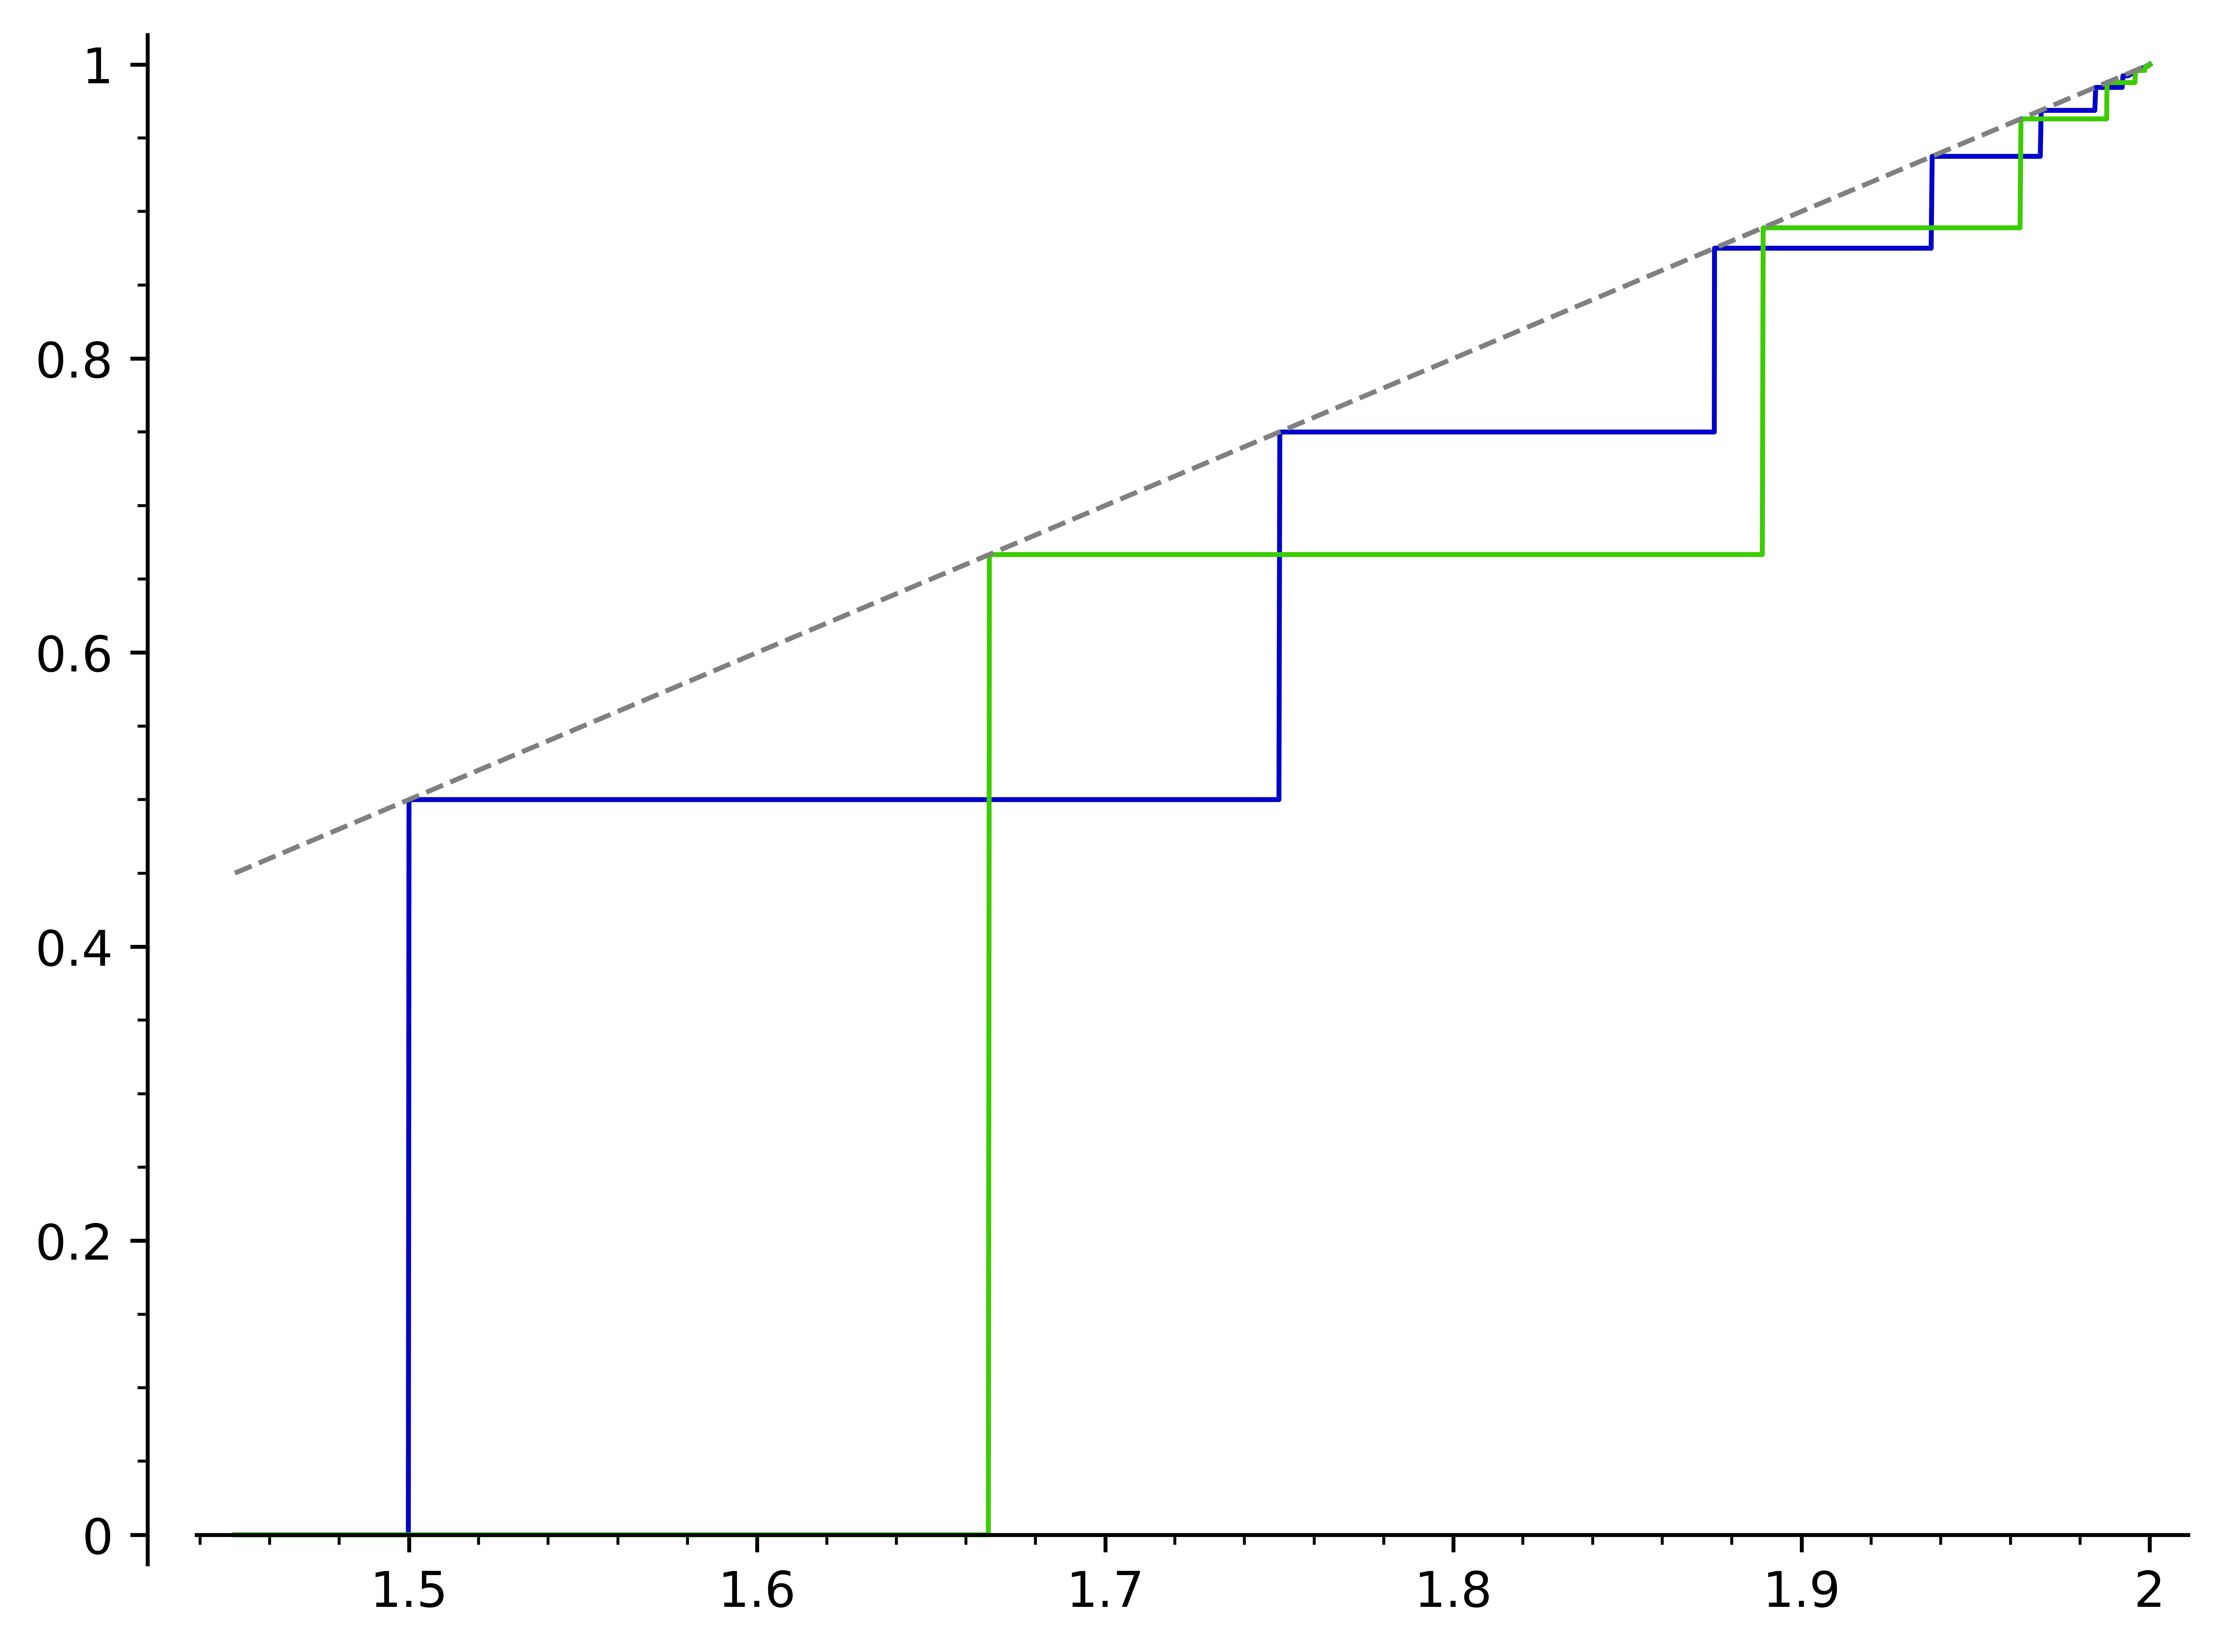
\includegraphics[width=\textwidth]{Pictures/geometric-series-distribution-2-3-half.png}
                    \caption{Geometric series construction \ref{item:geometricSeriesSufficientTailOrderConditionCounterexample}: Distribution functions $F_c$, $c=2, 3$.}
                    \label{fig:distributionsGeometricSeriesCounterexample-2-3}
                \end{subfigure}
                \begin{subfigure}[b]{0.49\textwidth}
                    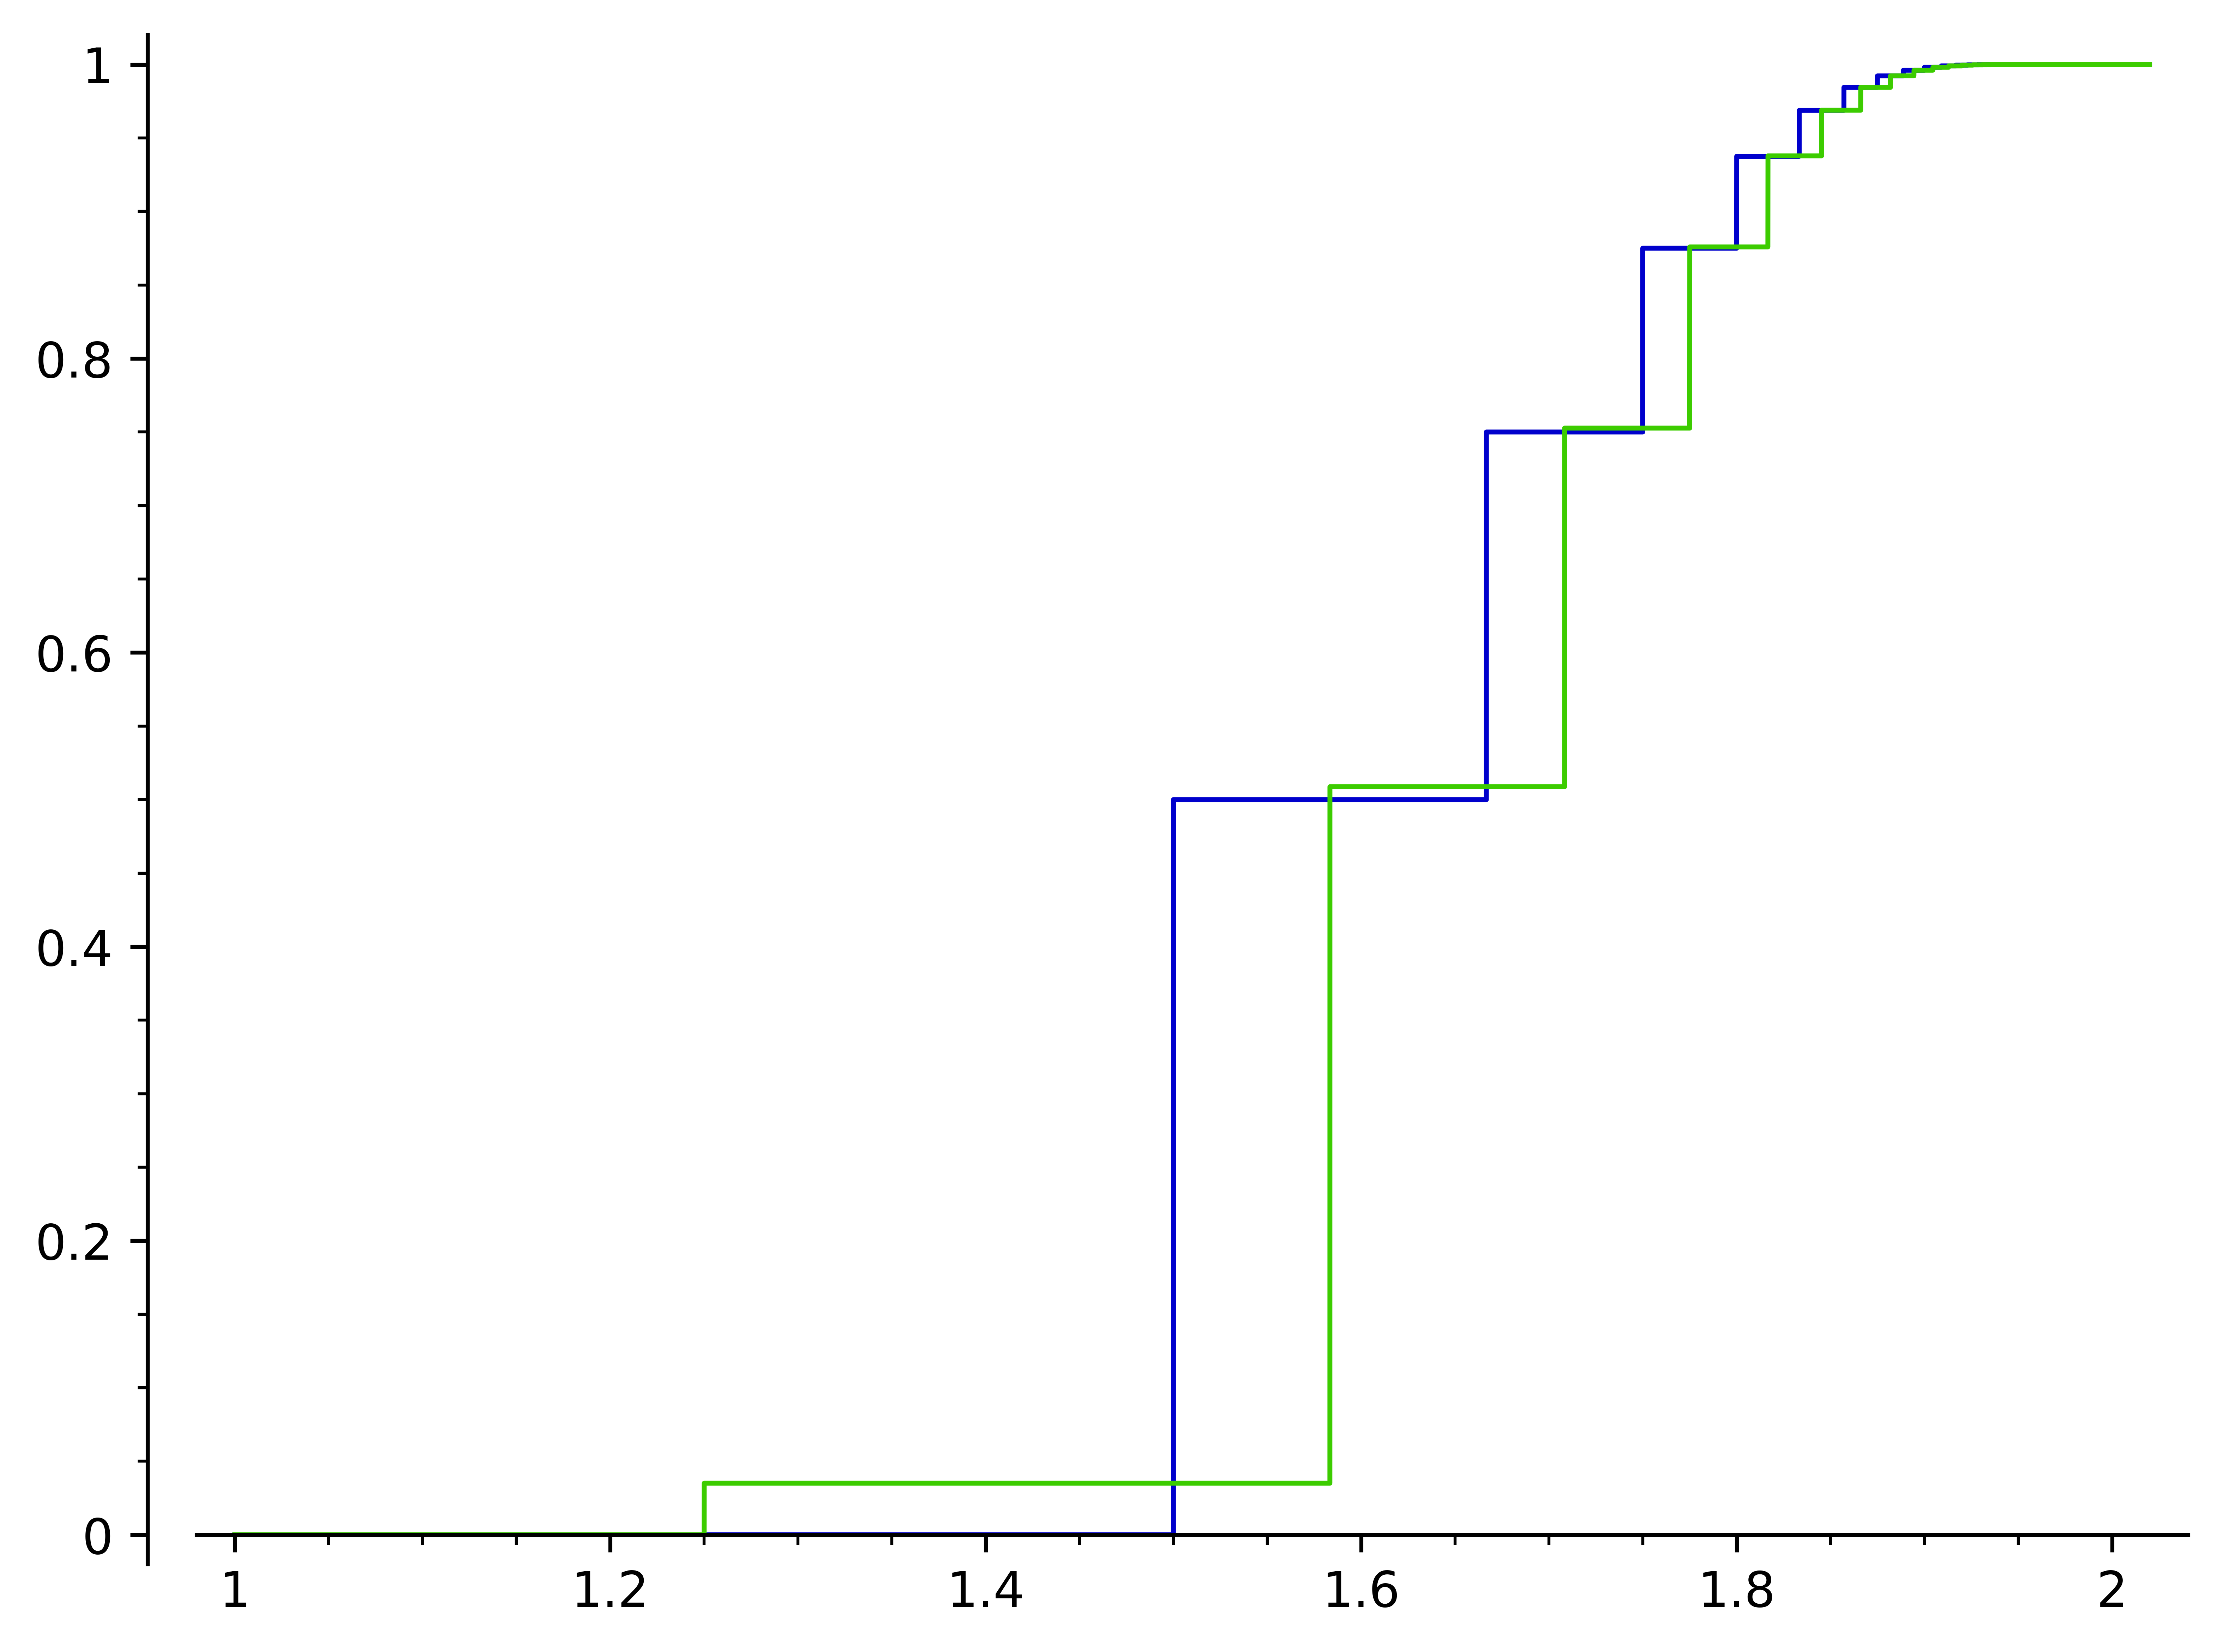
\includegraphics[width=\textwidth]{Pictures/little-shifts-distribution.png}
                    \caption{General discrete construction \ref{item:discreteSufficientTailOrderConditionCounterexample}: Distribution functions ($s_k = 1-\frac{1}{k+1}, f(s_k) = \frac{1}{2^k}$)}
                    \label{fig:littleShiftsCounterexample-distribution}
                \end{subfigure}
                
                \vspace*{0.01\textwidth}
                \begin{subfigure}[t]{0.49\textwidth}
                    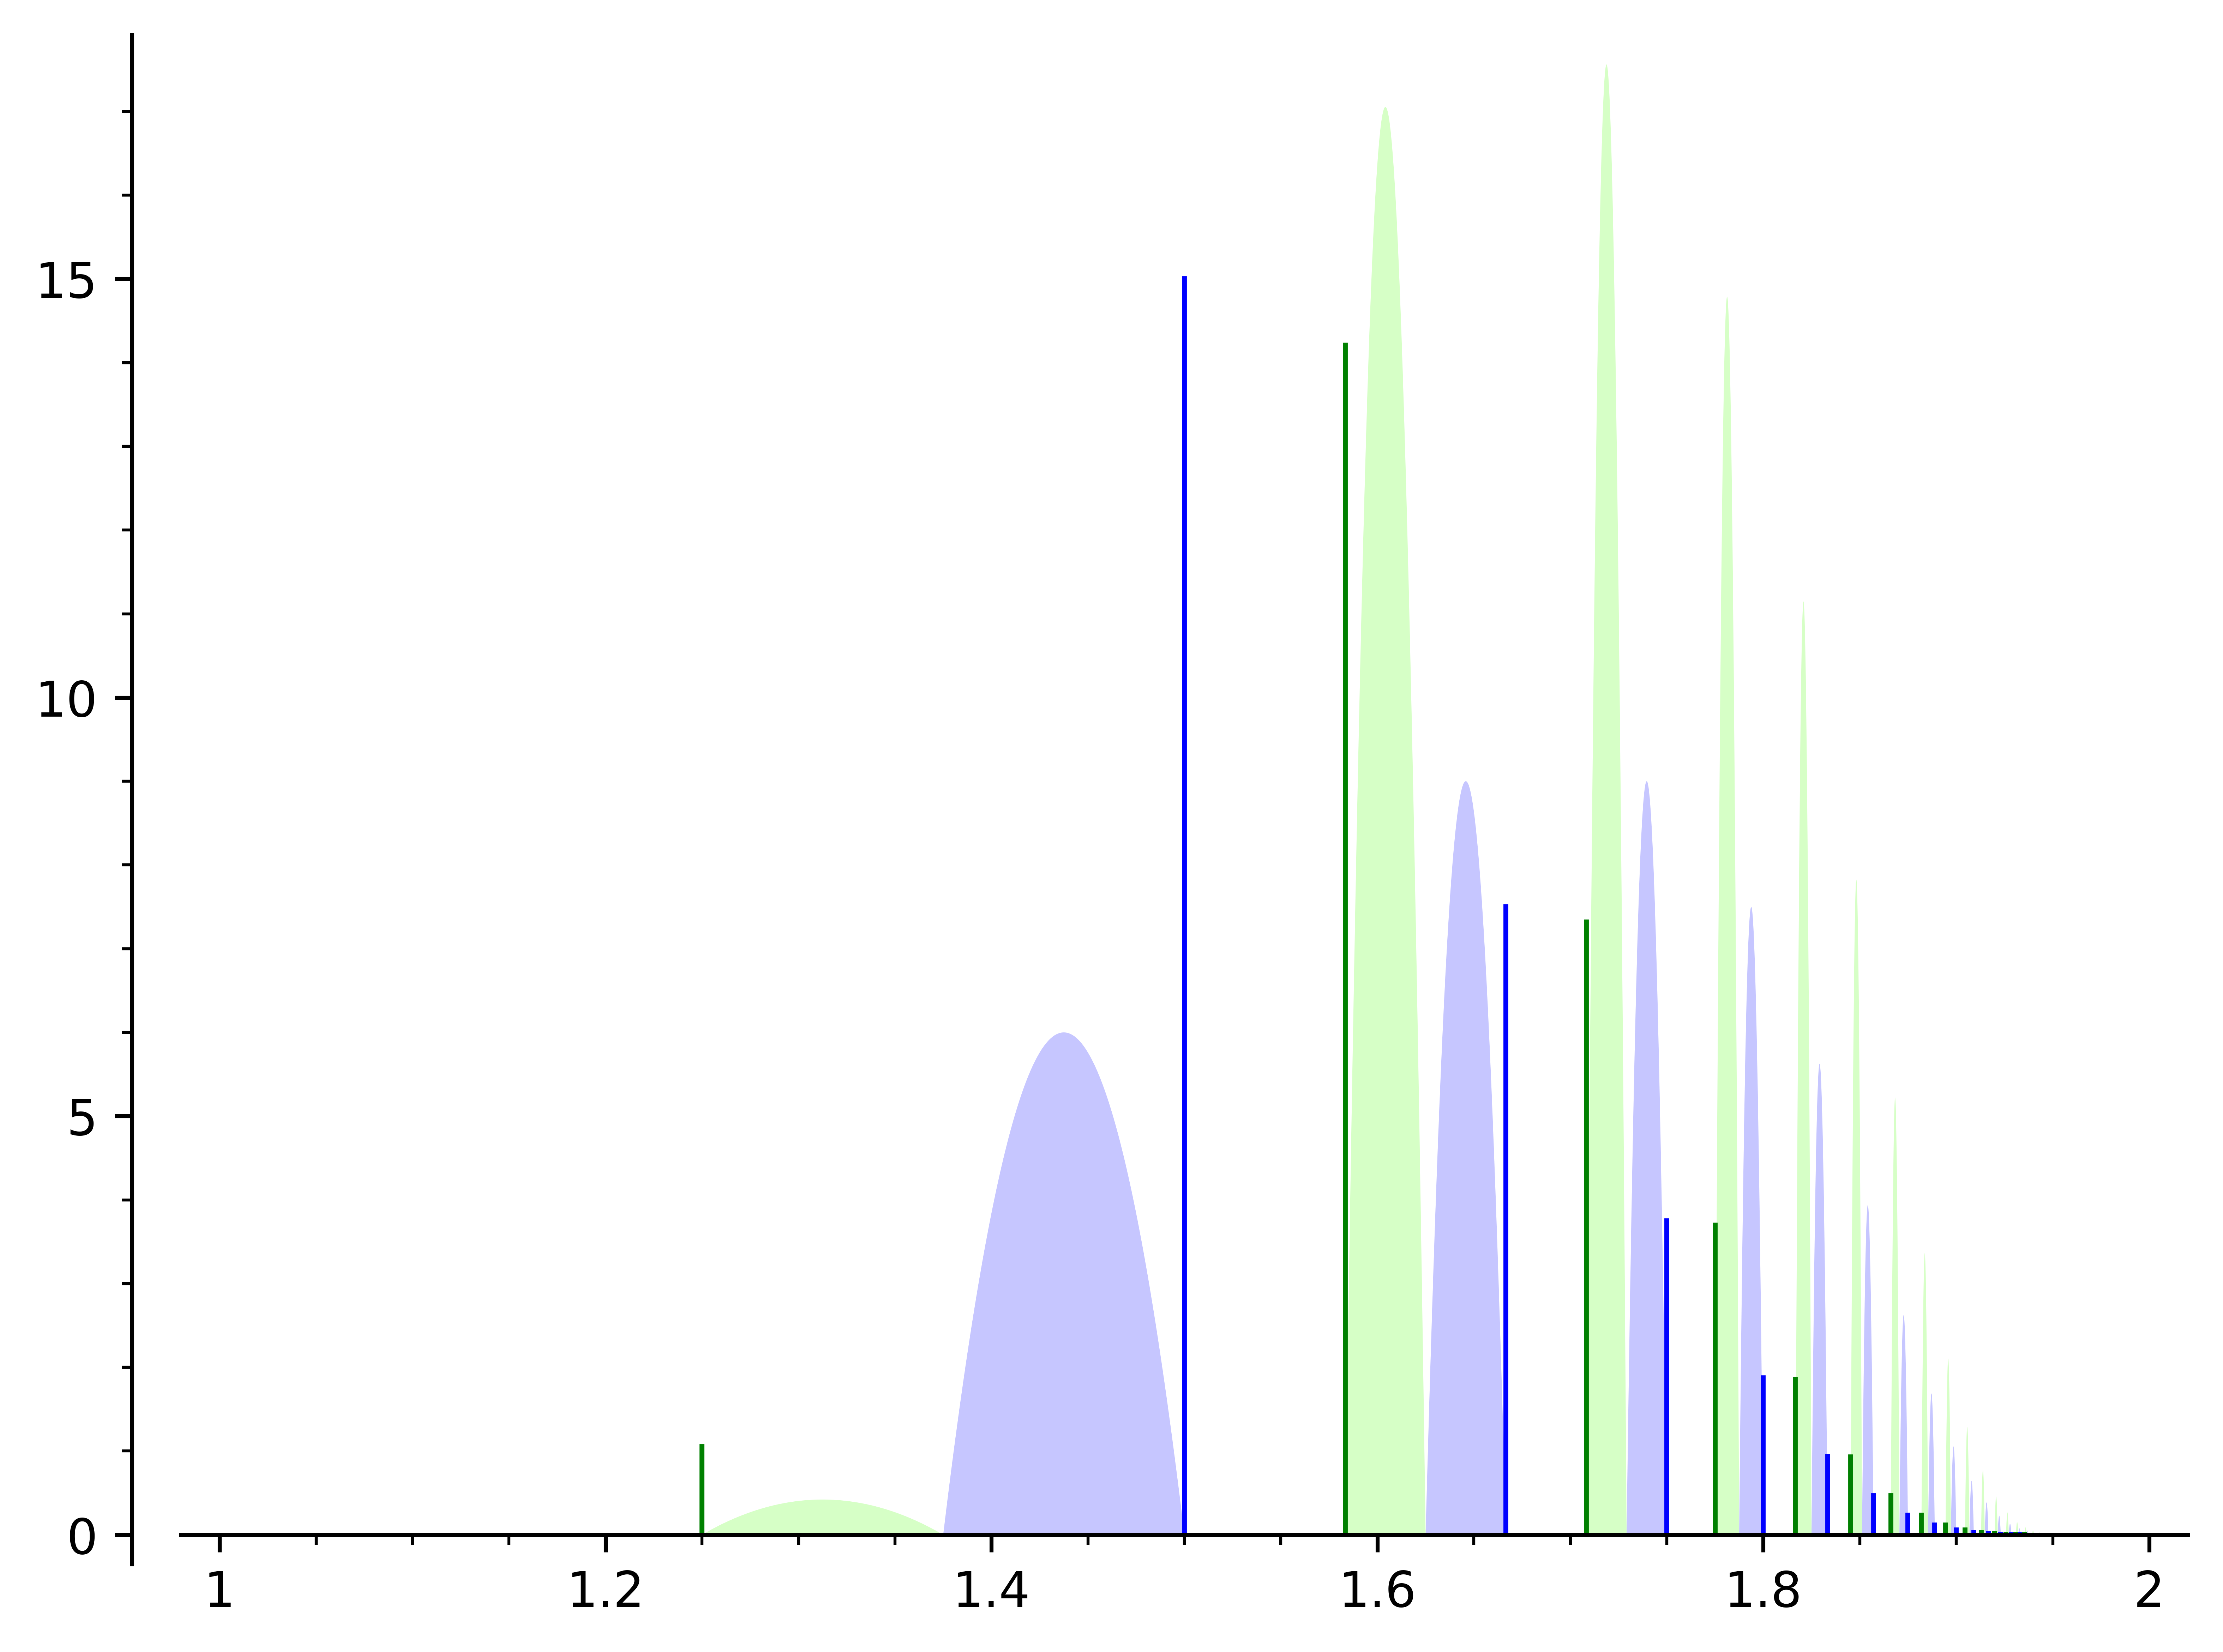
\includegraphics[width=\textwidth]{Pictures/ac-densities-masses.png}
                    \caption{Absolutely continuous construction: Densities (\ref{item:acSufficientTailOrderConditionCounterexample})/corresponding mass functions (\ref{item:discreteSufficientTailOrderConditionCounterexample}) (scaled by a factor of 30 to be visible)}
                    \label{fig:acCounterexample-masses-densities}
                \end{subfigure}
                \begin{subfigure}[t]{0.49\textwidth}
                    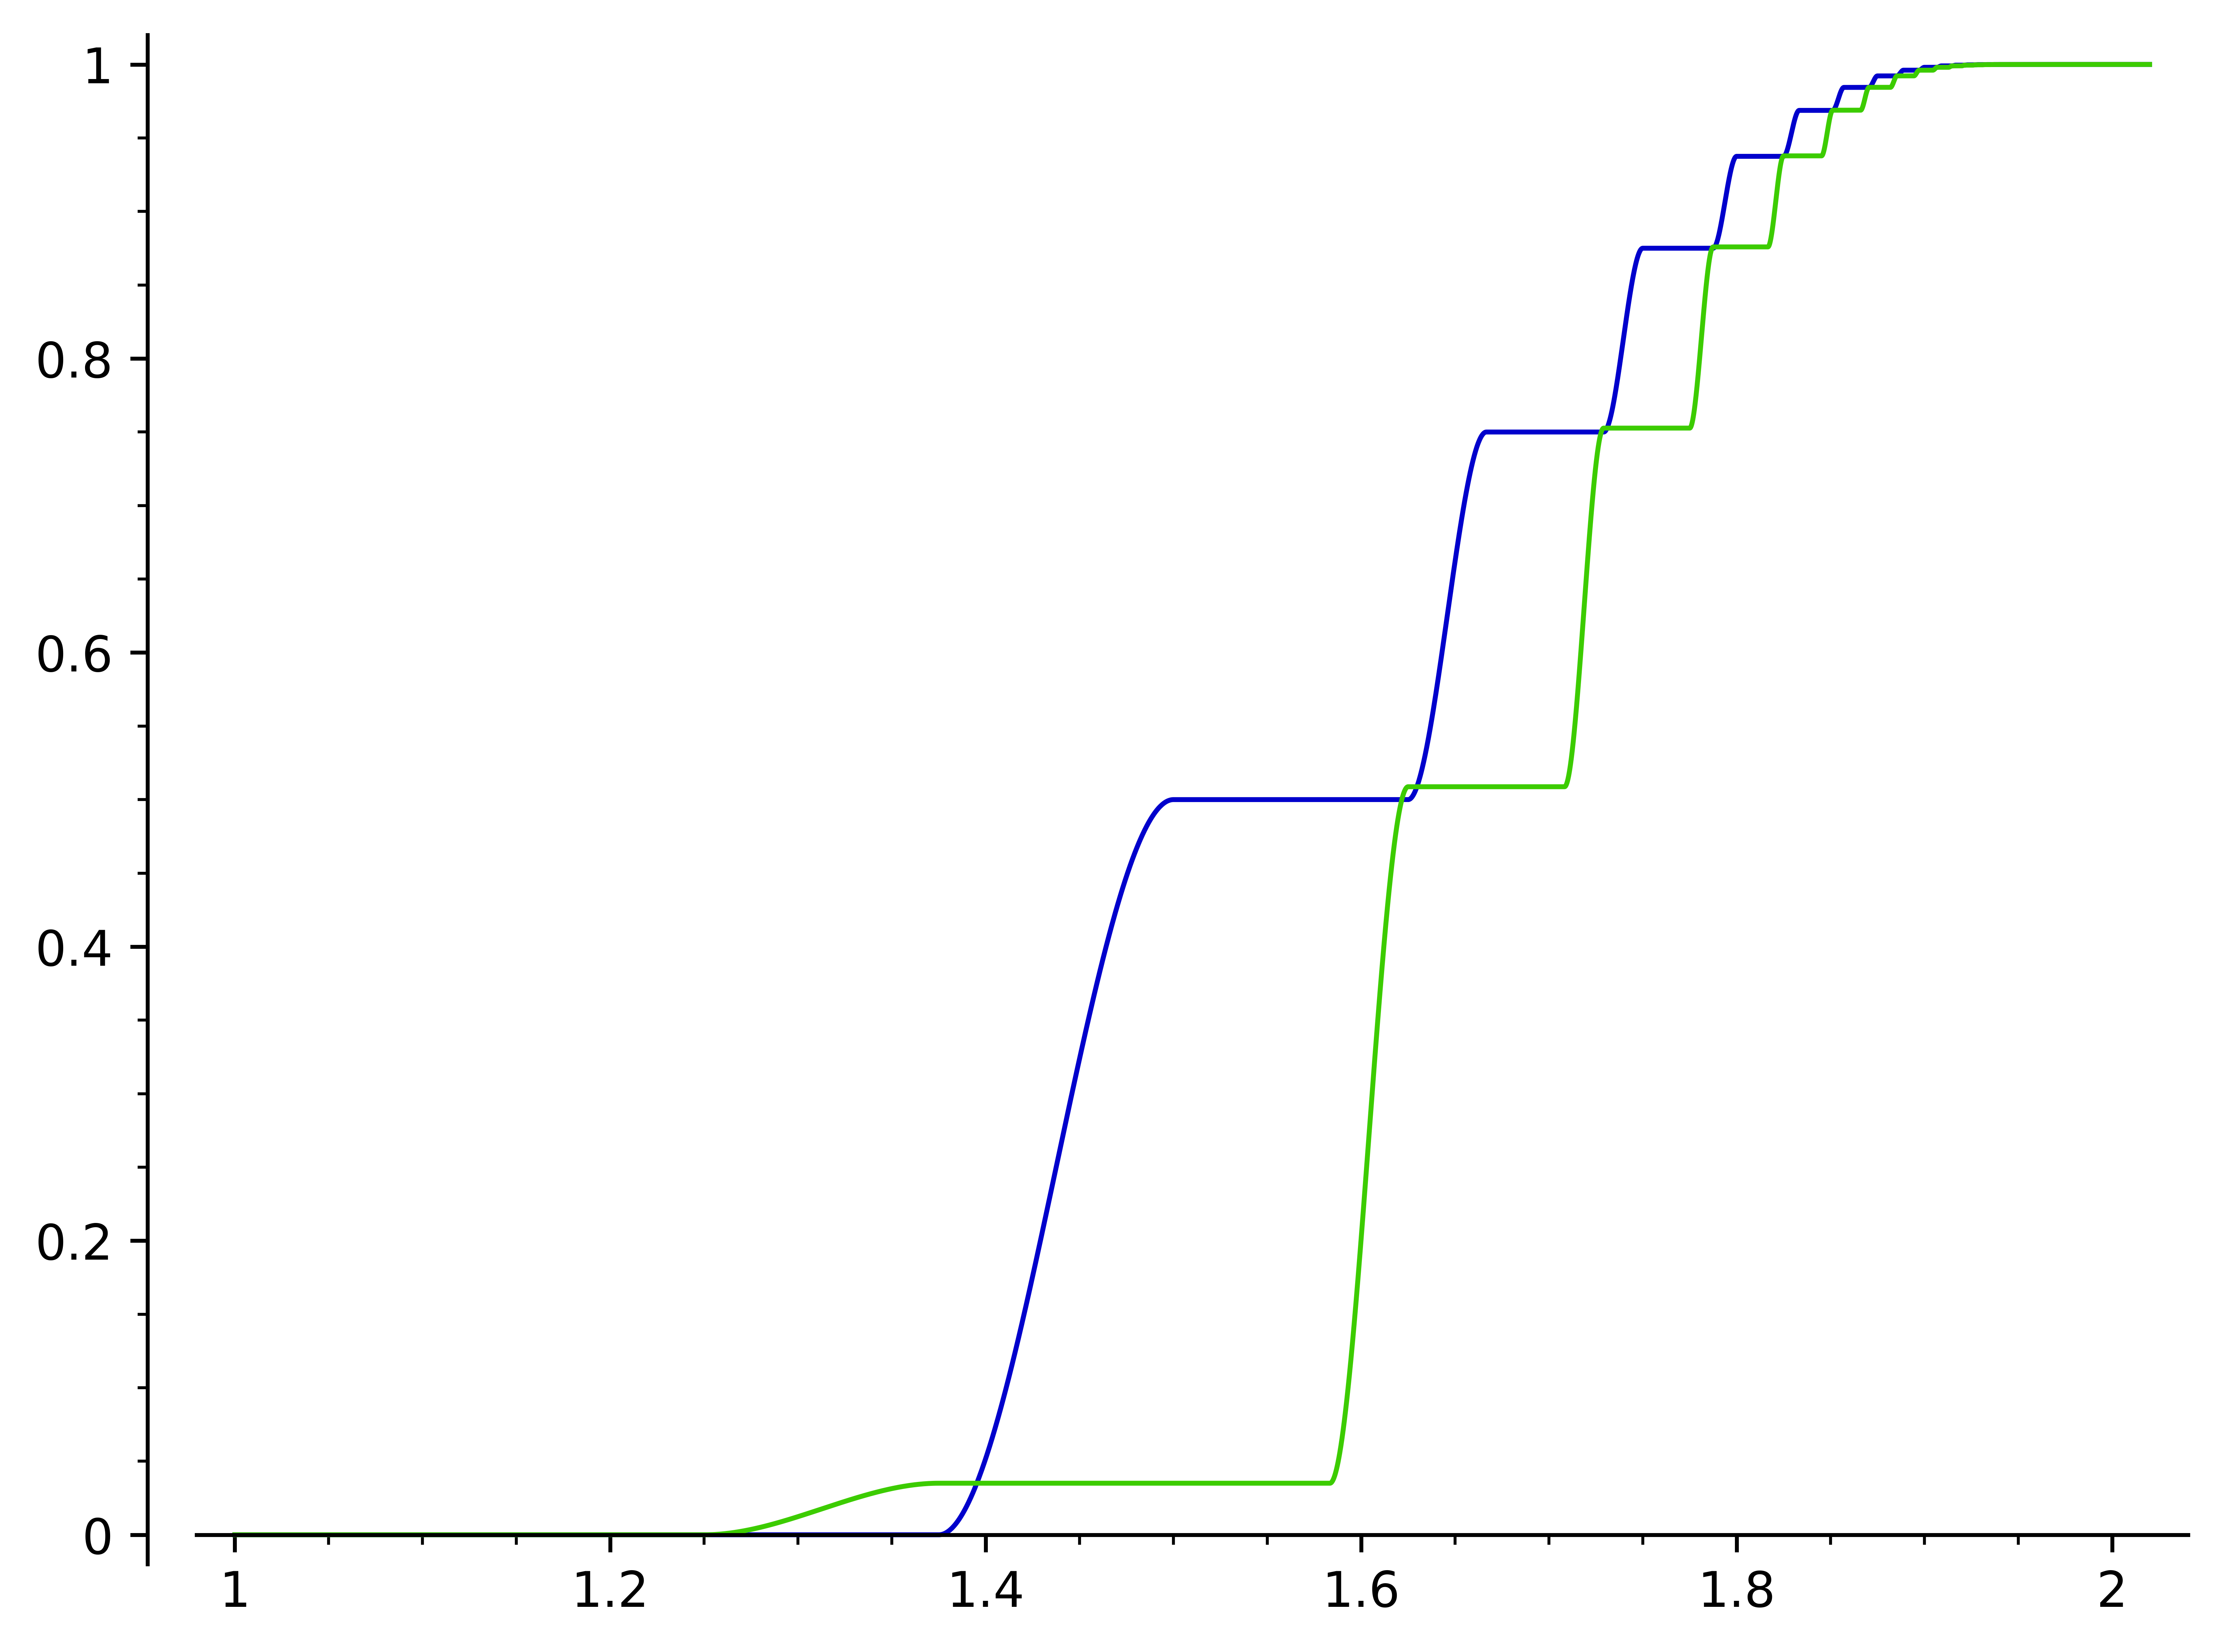
\includegraphics[width=\textwidth]{Pictures/ac-distribution.png}
                    \caption{Distribution functions of absolutely continuous construction \ref{item:acSufficientTailOrderConditionCounterexample}}
                    \label{fig:acCounterexample-distribution}
                \end{subfigure}
                
                \label{fig:sufficientTailOrderConditionsCounterexamples}
                \caption{Plots for the counterexamples from Example \ref{ex:tailOrderSufficientConditionsCounterexamples}}
            \end{figure}
    
            \item 
            \textbf{A process to produce two discrete distributions with pairwise alternating mass and distribution functions and bounded support which are $\leqtail$-comparable.}
            
            \label{item:discreteSufficientTailOrderConditionCounterexample}
            In this more general counterexample, we start with some discrete distribution $P$ with $\supp P = \set{s_1, s_2, \dots} \subseteq [a, b)$, $1 < a < b$, the $s_i$ in increasing order, and probability mass function $f$ which is strictly decreasing on the support, i.e. $\forall i < j: f(s_i) > f(s_j)$. We construct $\tilde{P}$ with mass function $g$, where each support point is shifted a bit to the right, with its probability adjusted to be only a little smaller, giving the remaining probability mass to the point $\tilde{a} \coloneqq \frac{1+a}{2}$.
            First, set $\tilde{s}_i \coloneqq \frac{s_i+ s_{i+1}}{2}$.
            We adjust the probability of $\tilde{s}_i$ by a factor $c_i < 1$, i.e. $g(\tilde{s}_i) = c_i f(s_i)$, chosen such that $c_i \geq \frac{s_i}{\tilde{s_i}}$ (ensuring $\tilde{P}$ has greater moments than $P$), $c_i \geq 1-\frac{1}{2^i}$ (ensuring the distribution functions alternate), and $c_i \geq \frac{f(s_{i+1})}{f(s_i)}$ (ensuring that $g$ 
            also is monotonic on its support). In summary, we have:            
            \begin{gather*}
                g(\tilde{s}_i) = c_i f(s_i), \quad
                c_i \coloneqq \max\biggset{\frac{s_i}{\tilde{s_i}}, 1-\frac{1}{2^i}, \frac{f(s_{i+1})}{f(s_i)}} < 1, \quad
                g(\tilde{a}) = \sum_{i \geq 1} (1-c_i) f(s_i).
            \end{gather*}
            By the first property of $c_i$, $g(\tilde{s}_i)\tilde{s}_i \geq f(s_i)s_i ~\forall i$, so for the moments we have:
            \begin{multline*}
                m_n(\tilde{P}) - m_n(P)
                = g(\tilde{a})*\tilde{a}^n + \sum_{k \geq 1} g(\tilde{s}_i) \tilde{s}_i^n - f(s_i) s_i^n \\
                \geq g(\tilde{a}) + \sum_{k \geq 1} f(s_i) s_i^n * (\tilde{s}_i^{(n-1)} - 1)
                \geq g(\tilde{a}) > 0.
%                \label{eq:momentPushingExample}
            \end{multline*}
            
            Secondly, the distribution functions alternate, see \autoref{fig:littleShiftsCounterexample-distribution}: on the one hand, 
            \begin{multline*}
                G(\tilde{s_k}) 
                = g(\tilde{a}) + \sum_{i=1}^k f(s_i)c_i 
                = g(\tilde{a}) - \bigpars{\sum_{i=1}^k (1-c_i) f(s_i)} + F(s_k) \\
                = \bigpars{\sum_{i \geq k+1} (1-c) f(s_i)} + F(s_k) > F(s_k) = F(\tilde{s_k}).
            \end{multline*}
            On the other hand, 
            \begin{multline*}
                G(s_k)
                = g(\tilde{a}) + \sum_{i=1}^{k-1} f(s_i)c_i 
                = g(\tilde{a}) + \sum_{i=1}^{k-1} f(s_i) - \sum_{i=1}^{k-1} f(s_i) (1-c_i) \\
                = F(s_k) - f(s_k) + g(\tilde{a}) - \sum_{i=1}^{k-1} f(s_i) (1-c_i) 
                = F(s_k) - f(s_k) + \sum_{i \geq k} f(s_i) (1-c_i).
            \end{multline*}
            Using the second property of $c_i$ and monotonicity of $f$, we get
            $\sum_{i \geq k} f(s_i) (1-c_i) \leq \sum_{i \geq k} f(s_i) \frac{1}{2^i} < \frac{1}{2^{k-1}} f(s_k) \leq f(s_k)$,
            therefore $G(s_k) < F(s_k)$.
            So in summary we have $P \lesstail \tilde{P}$, and their probability mass, as well as distribution functions are infinitely alternating.
%            , such that the sufficient condition of Theorem \ref{thm:acTailOrderSuffConditions} is not satisfied for any $x_0$.
            Furthermore, $\tilde{P}$ again satisfies the conditions we originally made on $P$: by repeating the process, we get a whole sequence of distributions which is ascending wrt. $\lesstail$, and no two distributions in it satisfy the sufficient condition of \ref{thm:acTailOrderSuffConditions} (and for any two \emph{consecutive} elements, the distribution functions are infinitely alternating as well).
            
            \item 
            \textbf{A process to produce two absolutely continuous distributions with pairwise alternating density and distribution functions, continuous densities and bounded support which are $\leqtail$-comparable.}
            
            \label{item:acSufficientTailOrderConditionCounterexample}
            For the absolutely continuous counterexample, we start with two discrete distributions $P_1, P_2$ where $P_2$ is obtained from $P_1$ by the process from \ref{item:discreteSufficientTailOrderConditionCounterexample}: In particular, we require $P_1 \lesstail P_2$, $\supp(P_1) = \set{s_1, s_2, \dots}$, $\supp(P_2) = \set{t_0, t_1, t_2, \dots}$ with $1 < t_0 < s_1 < t_1 < s_2 < t_2 < \dots$ ($t_0$ represents $\tilde{a}$ from above), and their distribution functions $F, G$ should alternate with $F(s_k) > G(s_k), F(t_k) < G(t_k) ~\forall k\geq 1$.
%            their mass functions $f, g$ should satisfy $f(s_i)s_i < g(t_i)t_i ~ \forall i$ (and therefore 
            
            We then shift the probability mass $P_1$ gives to each point $s_k$ to an interval to the left of $s_k$, and the probability mass $P_2$ gives to each point $t_k$ to an interval to the right of $t_k$, which preserves the order of the moments (illustrated in \autoref{fig:acCounterexample-masses-densities}). We do it in such a way that the distribution functions are again alternating, and the new density functions are continuous (\autoref{fig:acCounterexample-distribution}). We will call the new absolutely continuous distributions $\tilde{P}_1, \tilde{P}_2$, their new density functions $\tilde{f}, \tilde{g}$, and their distribution functions $\tilde{F}, \tilde{G}$.
            
            To formalize this, let $h: \R \to \R, x \mapsto (6x - 6x^2)\1_{[0, 1]}(x)$. $h$ is a simple probability density function ($\lintegral{\R}{h}{\lambda} = 1$), which is continuous since $h(0) = h(1) = 0$.
            Denote by $h_{[a, b]}: x \mapsto \frac{1}{b-a}h\bigpars{\frac{x-a}{b-a}}$ the version of $h$ scaled to the interval $[a, b]$, still integrating to 1.
%            Define $h_{a, b, s}: x \mapsto s*h(\frac{x-b}{b-a})*s$.
%            Another way to view it is that the integral of $h$ continuously interpolates between the values 0 and 1 on the interval $[0, 1]$.
            Also, let $m_{k} = \frac{t_{k-1} + s_k}{2}$.
            Using this notation, we define $\tilde{f}, \tilde{g}$ by:
            \begin{gather}
                \tilde{f} = \sum_{k \geq 1}  f(s_k) h_{[m_k, s_k]}, \quad
                \tilde{g} = \sum_{k \geq 0}  g(t_k) h_{[t_k, m_{k+1}]}.
                \label{eq:acSufficientTailOrderConditionCounterexample-densitiesDefinition}
            \end{gather}
            By construction, it's clear that $\lintegral{\R}{\tilde{f}}{\lambda} = \lintegral{\R}{\tilde{g}}{\lambda} = 1$, since $(f(s_k))_{k \geq 1}, g(t_k))_{k \geq 0}$ sum to $1$. The distribution functions are alternating:
            For $k \geq 1$,
            \begin{gather*}
                \tilde{F}(s_k) 
                = \lintegral{[1, s_k]}{\tilde{f}}{\lambda} 
                = \sum_{i=1}^{k} f(s_k) 
                = F(s_k)
                > G(s_k)
                = \sum_{i=1}^{k-1} g(t_k) 
                = \tilde{G}(s_k)
                ,\\                
                \tilde{G}(m_{k+1})                
                = \lintegral{[1, m_{k+1}]}{\tilde{g}}{\lambda} 
                = \sum_{i=1}^{k} g(t_k)
                = G(t_k)
                > F(t_k)
                = \sum_{i=1}^{k} f(s_k) 
                = \tilde{F}(m_{k+1}).
            \end{gather*}
            The ordering of the moments is preserved:
            \begin{multline*}
                m_n(\tilde{P_1})
                = \sum_{k \geq 1} \lintegral{[m_k, s_k]}{x^n h_{[m_k, s_k]}(x)}{\lambda(x)}
                < \sum_{k \geq 1} f(s_k)*s_k^n \\
                = m_n(P_1)
                < m_n(P_2) \\
                = \sum_{k \geq 0} g(t_k)*t_k^n
                < \sum_{k \geq 0} \lintegral{[t_k, m_{k+1}]}{x^n h_{[t_k, m_{k+1}]}(x)}{\lambda(x)}
                = m_n(\tilde{P_2}).
            \end{multline*}
            If the series in \eqref{eq:acSufficientTailOrderConditionCounterexample-densitiesDefinition} converges uniformly, continuity is preserved.
            For this we additionally need to have $\norm{f(s_k) h_{[m_k, s_k]}}_\infty = \frac{f(s_k)}{s_k - m_k} \toinfty{k} 0$, and similarly for $g$, which is the case if the probability masses $f(s_k)$ approach zero asymptotically faster than the consecutive differences of the $s_k$. For example, we can set $s_k = 2-\frac{1}{k+1}, f(s_k) = \frac{1}{2^k}$, and use $g, (t_k)_k$ constructed from it as in \ref{item:discreteSufficientTailOrderConditionCounterexample}.
            % TODO properly reference “uniform convergence preserves continuity”
        \end{enumerate}
    \end{ex}
    
    \subsection{Can the Tail Order Be Made a Total Order?}
    \label{subsec:tailOrderTotality}
    When we introduced the tail order, we already discussed its antisymmetry and totality properties: In short, $\leqtail$ in general is neither total nor antisymmetric; For antisymmetry, counterexamples of different distributions with equal moment sequences exist (as referenced before), while equal moment sequences of different distributions can not occur if the distributions have bounded supports. Yet this does not prove antisymmetry for distributions with bounded support, because $\leqtail$ could be indifferent between distributions with different moment sequences as long as the sequences disagree only finitely often.
%    however anti-symmetry \emph{does} hold on the reasonably large subset of distributions with bounded support.
    Similar questions can be posed concerning the totality of $\leqtail$. The only counterexamples we saw so far were trivially not $\leqtail$-comparable because they did not even have moments of all orders.
    A natural question thus is if there is some useful subset of $\DP$ where $\leqtail$ is total. As a first observation, $\leqtail$ can not be total on all of $\M$, because distributions can take negative values that can make the moment sequences alternating. 
    % TODO make this “alternating moment sequences” example even shorter [using Dirac measure notations]. Maybe  even move it further up, to the definition of tail order, discussing that \leqtail is not useful on negative values in the support
    As the simplest example, consider the point-mass distributions on $\delta_{-1}$ and $\delta_{0}$: The moment sequence of the former is given by $(-1)^n$, alternating around the sequence of the latter which is constantly $0$, making the distributions not $\leqtail$-comparable.
    A more subtle question, however, is if there is a smaller subset of $\DP$ where $\leqtail$ is total, which is easy to characterize and big enough to contain many useful distributions. We will discuss this question on the following pages.
    
    In \cite{bib:rassGameRiskManagI,bib:rassTotalOrderingOnLossDistributions}, the discussion focuses on the particular subset of distributions that have \emph{bounded support which is a subset of $[1, \infty)$} and are either \emph{discrete with finite support}, or \emph{absolutely continuous with a continuous density function}.
    In \cite[Lemma 2]{bib:rassTotalOrderingOnLossDistributions} and \cite[Lemma 2.4]{bib:rassGameRiskManagI}, the claim is that such distributions are always $\leqtail$-comparable.
    A proof is given for the absolutely continuous case; however, it contains an error, as it applies an argument similar to Theorem \ref{thm:acTailOrderSuffConditions} and implicitly assumes that of two density functions, one dominates the other from some point on
    \footnote{Meanwhile, the error was fixed in \cite{bib:rassGameRiskManagI}, and a new version was uploaded to arXiv stating all requirements (which means that the paper does not prove the totality of $\leqtail$).}.
    As shown in Example \ref{ex:tailOrderSufficientConditionsCounterexamples}, pairs of distributions exist where this is not the case, and which also are in $\Dgeqone$, bounded, and have continuous density functions.
    
    \subsubsection{The Moment Problem and its Variants}
    Since our question by the definition $\leqtail$ depends on moment sequences, it will be helpful to know about the properties of such sequences.
    The question to find out whether a given sequence $(m_n)_{n \in \N_0}$ is a moment sequence for some Borel measure $\mu$ on $\R$ is known as the \emph{moment problem}, and there are several variants studied in the literature:
%    to characterize moment sequences is known as the \emph{moment problem}, and there are several variants:
    The \emph{Hamburger moment problem} concerns measures supported on a subset of $\R$, the \emph{Stieltjes moment problem} is about measures supported on a subset of $[0, \infty)$,
    and the \emph{Hausdorff moment problem} deals with measures supported on a subset of $[0, 1]$. For all three versions, conditions are known that are both sufficient and necessary for $(m_n)_{n \in \N_0}$ to be a moment sequence of the respective kind.
    The moment problem has been extensively analyzed in the literature, for example in \cite{bib:shohatTheProblemOfMoments}, \cite{bib:akhiezerClassicalMomentProblem}, or the more recent \cite{bib:schmuedgenTheMomentProblem}.
    % TODO and negative values in the support make it useless, too.
%    We will introduce the characterizations by Stieltjes and Hausdorff, which are more interesting for us.
%    
%    \begin{defn}
%        % TODO check if the term “Hankel matrix” is appropriate. Isn't that an infinite matrix?
%        Let $n \geq 1$, $a_0, a_1, \dots, a_{2n} \in \R$. Define the \emph{Hankel matrix} $H(a_0,\dots,a_{2n})$ as
%        \begin{gather*}
%            H(a_0,\dots,a_{2n}) \coloneqq
%            \begin{pmatrix}
%            	a_0    & a_1     & a_2    & \dots    & a_n      \\
%            	a_1    & a_2     & \ddots &          & a_{n+1}  \\
%            	a_2    & \ddots  & \ddots & \ddots   & \vdots   \\
%            	\vdots &         & \ddots & \ddots   & a_{2n-1} \\
%            	a_n    & a_{n+1} & \dots  & a_{2n-1} & a_{2n}
%            \end{pmatrix}
%            \in \R^{(n+1)\times(n+1)}
%        \end{gather*}
%    \end{defn}
%    
%    \begin{thm}[Stieltjes Moment Characterization]
%        A sequence $(m_n)_{n \geq 0}$ of real numbers is the moment sequence of some measure $\mu$ on $[0, \infty)$ if and only if one of the following conditions hold:
%%        \begin{enumerate}
%%            \item
%%            \begin{gather*}
%%                
%%            \end{gather*}
%%        \end{enumerate}
%        \begin{gather}
%            \forall n: \det(H(m_0, \dots, m_{2n})) > 0,~ \det(H(m_1, \dots, m_{2n+1})) > 0 \\
%            \begin{split}
%                \forall n \geq m: \det(H(m_0, \dots, m_{2n})) > 0,~ \det(H(m_1, \dots, m_{2n+1})) > 0 \\
%                \text{ and } \forall n > m: \det(H(m_0, \dots, m_{2n})) = \det(H(m_1, \dots, m_{2n+1})) = 0
%            \end{split}
%        \end{gather}
%        In the first case, the measure $\mu$ has infinite support, in the second case, it has finite support of size $m$.
%    \end{thm}  

    \subsubsection{Non-Totality in the Stieltjes Case}
    The Hamburger moment problem is too general for our case, since negative values in the support can lead to alternating moment sequences, making the tail order non-total.
    However, we can make use of a result relating Stieltjes and Hamburger moment sequences:
    A moment sequence is called \emph{Hamburger-}/\emph{Stieltjes-determinate} if there is a \emph{unique} measure of the respective type generating the sequence \cite[p.68]{bib:schmuedgenTheMomentProblem}
    \footnote{More specifically, a unique \emph{Radon measure}, see \cite[A.1]{bib:schmuedgenTheMomentProblem}. This makes no difference in our case, since every finite Borel measure on $\R$, and therefore every measure in $\DP$, is a Radon measure, and also a moment sequence belongs to a probability measure if and only if $m_0 = 1$.}.
    The result we will use is that Stieltjes-determinateness in general does not imply Hamburger-determinateness:
    
    \begin{thm}[See \cite{bib:linMomentProblemRecentDevelopments}, citing {\cite[p.240]{bib:akhiezerClassicalMomentProblem}} and \cite{bib:chiharaIndeterminateHamburgerMomentProblems}]
        There exists a moment sequence $(m_n)_{n \in \N_0}$ that is Stieltjes-determinate, but not Hamburger-determinate.
    \end{thm}

    \begin{cor}
        There exist probability measures $P_1, P_2 \in \DP$ that have equal moment sequences and satisfy $P_1 \in \Dgeqzero, P_2 \notin \Dgeqzero$.
%        $\supp (P_1) \subseteq [0, \infty)$ and $\supp (P_2) \subsetneq [0, \infty)$.
        \label{cor:equalMomentSequencesStieltjesHamburger}
    \end{cor}
    \begin{proof}
        \sloppypar{
        Let $(m_n)_{n \geq 0}$ be a moment sequence which is Stieltjes-determinate, but not Hamburger-determinate.
        Let $\mu_1$ be the unique measure in $\Dgeqzero$ with that moment sequence.
%         and support in $[0, \infty)$.
        Let $\mu_2 \neq \mu_1$ be a different measure with that moment sequence, which exists since the sequence is not Hamburger-determinate. 
        Since $\mu_1$ is unique in the Stieltjes sense, the support of $\mu_2$ must overlap with $(-\infty, 0)$.
        If $m_0 \neq 1$, the measures constructed are not probability measures: 
        We normalize them and define $P_1 = \frac{1}{m_0}\mu_1, P_2 = \frac{1}{m_0}\mu_2$, which are probability measures which both have the moment sequence $(\frac{m_n}{m_0})_{n \geq 0}$.
    }
    \end{proof}
    
    This result allows us to show that two Stieltjes moment sequences can infinitely alternate: 
    \begin{ex}
%        We construct a pair of probability measures supported on a subset of $[0, \infty)$, which have infinitely alternating moment sequences:
        Let $P_1, P_2$ be the measures from Corollary \ref{cor:equalMomentSequencesStieltjesHamburger}, with moment sequence $(m_n)_{n \geq 0}$.
        Define a measure $\tilde{P}_2: A \mapsto P_2(A \cap [0, \infty)) + \1_A(0) P_2((\infty, 0))$, which shifts the whole probability mass $P_2$ puts on the negative half-axis to the point $0$, and has support in $[0, \infty)$.
        Then its moment sequence $(\tilde{m}_n)_{n \geq 0}$ is given by $\tilde{m}_0 = 1$, and for $n > 0$:
        \begin{gather*}
            \tilde{m}_n 
            = \lintegral{[0, \infty)}{x^n}{\tilde{P}_2}
            = \lintegral{[0, \infty)}{x^n}{P_2}
            = \lintegral{\R}{x^n}{P_2} - \lintegral{(-\infty, 0)}{x^n}{P_2}
            = m_n - \undersetbrace{\lintegral{(-\infty, 0)}{x^n}{P_2}}{\text{alternating}}.
        \end{gather*}
        By construction of $P_2$, the term $\lintegral{(-\infty, 0)}{x^n}{P_2}$ is strictly positive for $n$ even, and strictly negative for $n$ odd.
        Therefore $(\tilde{m}_n)_{n \geq 0}$ alternates infinitely around $(m_n)_{n \geq 0}$,
        and both sequences are moment sequences of probability measures supported on a subset of $[0, \infty)$.
    \end{ex}

    This shows that the space $(\Dgeqzero \cap \M)$ of probability measures supported on a subset of $[0, \infty)$ that have moments of all orders is still too large for $\leqtail$ to be total.
%    \todo{Give a counterexample explicitly.}
    
    \subsubsection{Distributions with Non-Negative Bounded Support}
    Next we look at distributions with support in a bounded interval $[a, b]$, $0 \leq a < b$.
    This is related to the Hausdorff moment problem where the bounded interval is $[0, 1]$.
    A sufficient and necessary condition for a sequence to be a Hausdorff moment sequence is based on repeatedly taking differences of successive terms.
    \begin{defn}
        The \emph{difference operator} $\Delta: \R^{\N_0} \to \R^{\N_0}$ maps a sequence of real numbers to the sequence of its successive differences:
        \begin{gather*} 
            \Delta((s_n)_{n \in \N_0}) \coloneqq (s_{n+1} - s_n)_{n \in \N_0}, ~ \text{ also written as }\,
            (\Delta s)_n \coloneqq s_{n+1} - s_n.
        \end{gather*} 
    \end{defn}

    \begin{thm}[\cite{bib:hausdorffMomentprobleme}]
        A sequence $m = (m_n)_{n \in \N_0}$ is a Hausdorff moment sequence, i.e. is the moment sequence of a measure $\mu$ on with support in $[0, 1]$,
        if and only if
        \begin{gather}
            \forall n, k \in \N: (-1)^k (\Delta^k m)_n \geq 0.
            \label{eq:completelyMonotonicSequence}
        \end{gather}
        A sequence that satisfies \eqref{eq:completelyMonotonicSequence} is called \emph{completely monotonic} \cite[Section III.4]{bib:widderTheLaplaceTransform}.
        \label{thm:hausdorffMomentSequenceCharacterization}
    \end{thm}
    \begin{proof}[Proof (necessity)]
        We only show here that condition \eqref{eq:completelyMonotonicSequence} is necessary, which is the easier part of the proof.
        Let $\mu$ be the measure with support in $[0, 1]$ which has $m$ as its moment sequence.
        We first proof by induction over $k$ that $(\Delta^k m)_n = \lintegral{[0, 1]}{x^n (x-1)^k}{\mu(x)}$:
        \begin{gather*}
            (\Delta m)_n 
            = m_{n+1} - m_{n} 
            = \lintegral{[0, 1]}{x^{n+1}}{\mu(x)} - \lintegral{[0, 1]}{x^n}{\mu(x)} 
            = \lintegral{[0, 1]}{x^n(x-1)}{\mu(x)}, \\
            (\Delta^{k+1} m)_n
%            = (\Delta^k m)_{n+1} - (\Delta^k m)_n \\
            = \lintegral{[0, 1]}{x^{n+1} (x-1)^k}{\mu(x)} - \lintegral{[0, 1]}{x^n (x-1)^k}{\mu(x)}
            = \lintegral{[0, 1]}{x^{n}(x-1)^{k+1}}{\mu(x)}.
        \end{gather*}
        From this we directly get that $(-1)^k (\Delta^k m)_n = \lintegral{[0, 1]}{x^n (1-x)^k}{\mu(x)}$.
        Since we integrate over $[0, 1]$, the integrand is non-negative on the domain of integration.
        Therefore, $(-1)^k (\Delta^k m)_n \geq 0$.
    \end{proof}

    While Hausdorff's characterization works for distributions with support in $[0, 1]$, we are actually interested in distributions supported in $[1, b]$ for some $b > 1$.
    Moment sequences behave somewhat differently in that case: For example, while they are monotonically decreasing in the former case, they are monotonically increasing in the latter, even growing without bound if there is some mass to the right of $1$.
    We can obtain a first necessary criterion, which looks similar to \eqref{eq:completelyMonotonicSequence}, for a sequence to be the moment sequence of such a distribution:
    \begin{cor}
        \label{cor:hausdorff-1-b-necessaryCondition}
        For any moment sequence $m$ of a measure $\mu \in \DP_{[1, b]}$, all successive differences are non-negative:
        \begin{gather}
            \forall n, k \in \N: (\Delta^k m)_n \geq 0.
        \end{gather}
    \end{cor}
    \begin{proof}
        As in the last proof, we have that $(\Delta^k m)_n = \lintegral{[1, b]}{x^n (x-1)^k}{\mu(x)}$.
        Since in this case, $x-1 > 0 \,\forall x \in [1, b]$, the integrand is non-negative, and $(\Delta^k m)_n \geq 0$.
    \end{proof}

    Another similar necessary condition can be stated for moment sequences of distributions on $[0, b]$, using a somewhat modified difference operator:
    \newcommand{\DeltaB}[1]{\Delta\hspace{-.225cm}{\mathrel{\raisebox{0.045cm}{\scalebox{.9}{$\scriptscriptstyle#1$}}}\hspace{.22cm}}\hspace{-0.09cm}}
    \begin{lemma}
        \label{lemma:hausdorff-0-b-necessaryCondition}
        Let $b \geq 0$, $\DeltaB{b}: \R^{\N_0} \to \R^{\N_0}$, $(\DeltaB{b} m)_n \coloneqq m_{n+1} - b * m_n$.
        Then for any moment sequence $m$ of a measure $\mu \in \DP_{[0, b]}$:
        \begin{gather}            
            \forall n, k \in \N: (-1)^k (\DeltaB{b}^k m)_n \geq 0.
        \end{gather}
    \end{lemma}
    \begin{proof}
        Analogously to the proof of \ref{thm:hausdorffMomentSequenceCharacterization},
        we can prove by induction that $(\DeltaB{b}^k m)_n = \lintegral{[0, b]}{x^n (x-b)^k}{\mu(x)}$.
        Since the integrand in the expression $(-1)^k (\DeltaB{b}^k m)_n = \lintegral{[0, b]}{x^n (b - x)^k}{\mu(x)}$ is non-negative, we can conclude $(-1)^k (\DeltaB{b}^k m)_n \geq 0$.
    \end{proof}

    % TODO basically, we woould need a sufficient condition to construct a counterexample; if we can proof that no alternating counterexample exists, a necessary condition will be enough.
    While \ref{cor:hausdorff-1-b-necessaryCondition} and \ref{lemma:hausdorff-0-b-necessaryCondition} give necessary conditions, it would be very useful to have a condition that is also sufficient. However, using \ref{lemma:hausdorff-0-b-necessaryCondition} we can show that \ref{cor:hausdorff-1-b-necessaryCondition} is not sufficient:
    
    \begin{ex}
        We construct a sequence that satisfies the condition of \ref{cor:hausdorff-1-b-necessaryCondition} and is infinitely alternating around a moment sequence:
        Let sequences $s, q$ be given by $s_n = 4^n$ for $n \in \N_0$, $q_n = (-1)^n\frac{1}{2^n}$ for $n \in \N$ and $q_0 = 0$. $s$ is the moment sequence of $\delta_4$. We show that $(s + q)$ satisfies the conditions of \ref{cor:hausdorff-1-b-necessaryCondition}:
        Let $k \in \N$.
        By induction, one can show that $(\Delta^k s)_n = 3^k 4^n$ for all $n \in \N_0$, as well as $(\Delta^k q)_n = 3^k\frac{(-1)^{n+k}}{2^{n+k}}$ for $n \in \N$, and $(\Delta^k q)_0 = 3^k \frac{(-1)^k}{2^k} - (-1)^k$.
        Since $\Delta$ is a linear operator, we have $(\Delta^k (s+q))_n = (\Delta^k s)_n + (\Delta^k q)_n$ for all $n, k \in \N_0$. This sum is non-negative:
        If $n \geq 1$, we get $(\Delta^k (s+q))_n = 3^k\bigpars{4^n + \frac{(-1)^{n+k}}{2^{n+k}}} \geq 0$, since $4^n \geq 1, \frac{(-1)^{n+k}}{2^{n+k}} > -1$.
        If $n = 0$, we have $(\Delta^k (s+q))_n = 3^k\bigpars{1 + \frac{(-1)^{k}}{2^{k}}} - (-1)^k$, which is non-negative as well:
        For $k = 0$, this becomes $1*(1 + 1) - 1 = 1$.
        For $k \geq 1$, we have $1 + \frac{(-1)^{k}}{2^{k}} \geq \frac{1}{2}$ and therefore $3^k\bigpars{1 + \frac{(-1)^{k}}{2^{k}}} - (-1)^k \geq \frac{3}{2} - (-1)^k > 0$.
        
%        for $k = 1$, $3*(1 - \frac{1}{2}) + 1 = \frac{7}{2}$
        
%          \geq 0$ for all $n, k$.
        So $(s+q)$ satisfies the condition of Corollary \ref{cor:hausdorff-1-b-necessaryCondition}. 
        By construction, it infinitely alternates around the moment sequence $s$, because $q$ alternates infinitely around 0.
        As the sequence also satisfies $s_0 + q_0 = s_0 = 1$ (necessary to be the moment sequence of a probability measure), these properties make it a candidate for a counterexample to the tail order being total for probability measures with non-negative, bounded support. 
        
        However, $(s+q)$ does not satisfy \ref{lemma:hausdorff-0-b-necessaryCondition} for any reasonable choice of $b$:
        If $(s+q)$ was the moment sequence of some measure $\mu$ with support in $[0, b]$, then $\forall n \geq 0: s_n + q_n < b^n$.
        We can take the bound $s_n + q_n \leq 5^n$, which is satisfied since $s_n \leq 4^n, q_n < 1$. So the support of $\mu$ must be a subset of $[0, 5]$.
        However, calculations show that $(-1)^2 (\DeltaB{5}^2 (s+q))_1$ is negative:
        We have $(s+q)_1 = 4 - \frac{1}{2} = \frac{7}{2}$, $(s+q)_2 = 16 + \frac{1}{4} = \frac{65}{4}$ and $(s+q)_3 = 64 - \frac{1}{8} = \frac{511}{8}$.
        From this we get $(\DeltaB{5} (s+q))_1 = \frac{65}{4} - 5 * \frac{7}{2} = - \frac{5}{4}$ and $(\DeltaB{5} (s+q))_2 = \frac{511}{8} - 5 * \frac{65}{4} = - \frac{139}{8}$, and finally $(\DeltaB{5}^2 (s+q))_1 = - \frac{139}{8} + 5*\frac{5}{4} = - \frac{89}{8}$.
        Therefore, $(-1)^2 (\DeltaB{5}^2 (s+q))_1  = - \frac{89}{8} < 0$, violating the necessary condition of Lemma \ref{lemma:hausdorff-0-b-necessaryCondition}.        
        So $(s+q)$ is not a moment sequence of a measure in $\DP_{[0, b]}$, and the condition in Corollary \ref{cor:hausdorff-1-b-necessaryCondition} can not be sufficient.
    \end{ex}

    \subsubsection{Possible Further Progress}

    As far as this thesis is concerned, the question whether two moment sequences of distributions on either an interval $[0, b]$ or an interval $[1, b]$ can infinitely alternate could not be settled. It therefore remains open for the moment if $\leqtail$ is a total order on such distributions.
    However, the condition of complete monotonicity \eqref{eq:completelyMonotonicSequence} seems quite strict, and during experimentation I could not even find a pair of completely monotonic sequences alternating more than twice; some possible further progress could be to prove that two Hausdorff moment sequences (i.e. for the $[0, 1]$-case) can not infinitely alternate. Possibly, such a result could then be generalized to the $[0, b]$-case using the condition of \ref{lemma:hausdorff-0-b-necessaryCondition}, which would directly yield totality for the $[1, b]$-case as well.
    
    While the necessary condition of \ref{lemma:hausdorff-0-b-necessaryCondition} could be sufficient to transfer a positive result from $[0, 1]$ to $[0, b]$, it surely does not suffice if a counterexample is found: Even if we found two alternating sequences satisfying the conditions of \ref{lemma:hausdorff-0-b-necessaryCondition}, this would still not ensure that corresponding Borel measures exist, since we only proved the condition to be necessary, not sufficient.
    Another point is that if counterexamples exist, it would be desirable to find a counterexample with absolutely continuous distributions, because only such an example could show that $\leqtail$ is also non-total if we restrict ourselves to those distributions in $\DP_{[0, b]}$ which are absolutely continuous or finitely supported (recall that $\leqtail$ \emph{is} total in the case of finite supports, by virtue of Corollary \ref{cor:discreteFiniteTailOrder-RLexEquivalence}).
%    Yet another issue is that we are especially interested in distributions that 
%%    either have finite support, or 
%    are absolutely continuous (or with finite support, but there no counterexamples exist by \ref{thm:discreteTailOrderSuffConditions}); so even if we found a counterexample and proved that the two sequences belonged to measures on $[0, b]$, this would still not ensure the measures are absolutely continuous.
    
    It is important to note that characterizations for moment sequences of measures supported on an arbitrary compact interval $[a, b]$ do exist.
    Two conditions equivalent to a real sequence $m$ being an $[a, b]$-moment sequence are given in \cite[Theorem 3.13]{bib:schmuedgenTheMomentProblem}:
    The first condition requires that both $m$ and $((a+b)E(m) - E(E(m)) - ab*m)$ are positive semidefinite sequences, where $E: (s_n)_{n \in \N_0} \mapsto (s_{n+1})_{n \in \N_0}$ denotes the shift operator.
    The second condition requires that $L_m(p^2) \geq 0$ and $L_m((b-x)(x-a)q^2) \geq 0$ for all real polynomials $p, q \in \R[x]$. Here $L_m$ is the \emph{moment functional}, the linear functional $L_m: \R[x] \to \R$ uniquely defined by $L_m(x^n) \coloneqq m_n$ for all $n \in \N_0$.
    These characterizations could be a different way to prove the totality of $\leqtail$ on $\DP_{[0, b]}$.
%     one requiring the positive semidefiniteness of the sequence itself as well as a second sequence derived from it, and the other one requiring that two expressions involving the so-called \emph{moment functional} of the sequence be non-negative for all real polynomials.
    
%    An interesting note is that in some references it is suggested that Hausdorff's characterization can easily be generalized to any interval $[a, b]$ (for example, the review \cite{bib:bultheelBookReviewMomentProblem} on Schmüdgen's book \cite{bib:schmuedgenTheMomentProblem}).
%    However, I could not yet find a formalization of this as a necessary and sufficient criterion. If something in this direction could be found, this would definitely be a helpful step, either for transferring a proof from $[0, 1]$ to $[1, b]$, or for proving counterexample sequences to have corresponding measures.
     
    
    \section{Nash Equilibria in Tail-Ordered Games}
    We will now analyze Nash equilibria of distribution-valued games with respect to the stochastic tail order.
    An important result of this section is that, unlike their real-valued counterparts, these games fail to have mixed-strategy Nash equilibria in general.
    
    We restrict our attention to games with finitely supported distributions as payoffs, and we will show that such games already fail to have mixed-strategy Nash equilibria in many cases.
    As shown in Corollary \ref{cor:discreteFiniteTailOrder-RLexEquivalence}, for finitely supported distributions, the tail order can be reduced to a lexicographic comparison.
    To make our discussion notationally easier, we represent games with finite common support of the payoff distributions as real-valued vectors of probabilities, ordered by the reflected lexicographic order. This is justified since the distribution-valued game and its corresponding vector-valued game are isomorphic and therefore have the Nash equilibria, as the subsequent lemma shows.
    \begin{defn}
        A \emph{vector-valued game} of dimension $m \in \N$ is a game $G$ with generalized payoffs in $\R^m$.
        If it is equipped with the preorder $\leqRlex$, we call it a \emph{reflected-lexicographically ordered} (also \emph{ref-lex-ordered}) game.
    \end{defn}

    \begin{notation}
        If $G$ is a distribution-valued game, we write
        \begin{gather*}
            \supp(G) \coloneqq \bigcup\limits_{\substack{s \in S,\\k \in [n]}} \supp(u_k(s))
        \end{gather*}
        for the common support of its payoff distributions.
    \end{notation}

    \begin{defn}
        Let $G$ be a distribution-valued game with finite common payoff support $\supp(G) = \set{x_1, \dots, x_m}$, $x_1 < \dots < x_m$.
        For each $k \in [n], s \in S$, let the payoff $u_k(s)$ have the probability mass function $f_{k, s}$.
        Then the \emph{probability vector game corresponding to $G$} is the vector-valued game $H$ with the same strategies as $G$ that has the payoffs $v_k(s) \coloneqq (f_{k, s}(x_1), \dots, f_{k, s}(x_m))$ for all $k \in [n], s \in S$.
    \end{defn}

    \begin{lemma}
        Let $G$ be a distribution-valued game such that $\supp(G)$ is finite, and $\supp(G) \subseteq [1, \infty)$.
        Let $H$ be the probability vector game corresponding to $G$.
        Then  $G_{\leqtail}$ and $H_{\leqRlex}$ are isomorphic.
    \end{lemma}
    \begin{proof}
        Let $\DP_{\supp(G)}$ denote the measures from $\DP$ supported on $\supp(G)$.
        Denote by $B \coloneqq \set{(p_1, \dots, p_m) \in [0, 1]^m \mid \sum_{i=1}^{m} p_i = 1} \subseteq \R^m$ the set of $m$-dimensional probability vectors.
        Then $\phi: \DP_{\supp(G)} \to B, P \mapsto (P(\set{x_1}), \dots, P(\set{x_n}))$ is a bijective function, satisfying $\phi(u_k(s)) = v_k(s)$ for all $k \in [n], s \in S$ by construction of $v_k(s)$.
        Since the payoffs of $G$ are from $\DP_{\geq 1}$, we can apply Corollary \ref{cor:discreteFiniteTailOrder-RLexEquivalence}:
%        , mapping distributions ordered by $\leqtail$ to real-valued vectors ordered by $\leqRlex$ preserves the ordering, 
        This shows that for all $s, t \in S, k \in [n]$, it holds that $u_k(s) \leqtail u_k(t)$ if and only if $v_k(s) \leqRlex v_k(t)$.
    
    \end{proof}

    \begin{defn}
        Let $G$ be an $m$-dimensional vector-valued game. For $i \in [m]$, let its \emph{$i$-th coordinate projected game}
        be defined as the real-valued game $G_i$ with the same strategies as $G$, and payoffs
        $u^i_k(s) \coloneqq (u_k(s))_i$ for all $k \in [n], s \in S$.
    \end{defn}

    \subsection{Existence Conditions for Mixed-Strategy Nash Equilibria in Lexicographically-Ordered Games}
    Not all ref-lex-ordered games have mixed-strategy Nash equilibria, which is an important difference from the theory of real-valued games. We will first illustrate this with an example, and then work out under which circumstances such Nash equilibria do exist.
    % TODO better game table design
    
    \newcommand{\Gproj}[1]{G_{#1}}
    \newcommand{\Gprojsub}[1]{\bar{G}_{#1}}
    
    \begin{ex}
        \label{ex:reflectedLexicographicallyOrderedGameWithoutEquilibria}
%        Consider the vector-valued two-player zero-sum game $G$ represented by
        The following game is an example of a ref-lex-ordered game:
        \begin{gather}
            \centering
            \begin{tabular}{c|c|c|}
            	      &        $b_1$        &        $b_2$        \\ \hline
            	$a_1$ & (0.1,\; 0.8,\; 0.1) & (0.1,\; 0.7,\; 0.2) \\ \hline
            	$a_2$ & (0.6,\; 0.1,\; 0.3) & (0.8,\; 0.1,\; 0.1) \\ \hline
            \end{tabular}
        \end{gather}
        The game is a two-player matrix game (i.e. zero-sum), so we only specify payoffs for the first player.
        An isomorphic tail-ordered distribution-valued game can be constructed from it for any specified support set of size 3 that lies in $[1, \infty)$,
        and which specific support is chosen does not matter for the tail order.
        
        This game has no Nash equilibria with respect to $\leqRlex$.
        To see this, we will first take a closer look at the highest coordinate, projecting the game to it: Consider the projected game
        $\Gproj{3}$ represented by $\smallmat{0.1 & 0.2 \\ 0.3 & 0.1}$, which is a real-valued zero-sum game that we can solve with standard techniques.
        
        Computations done with the game-theoretic library included in the mathematical software {SageMath} (which implements the enumeration support algorithm from subsection \ref{subsec:exactComputationNashEquilibriaSupportEnumerationAlgorithm}, see \cite{bib:sageNormalFormGameDocumentation})
        show that $\Gproj{3}$ has exactly one Nash equilibrium, with mixed strategies $s_1 = \bigpars{\frac{2}{3}, \frac{1}{3}}$ for player 1 and $s_2 = \bigpars{\frac{1}{3}, \frac{2}{3}}$ for player 2, yielding a payoff of $\frac{1}{6}$ to player 1.
        Applying this strategy to our original game $G$ yields the payoff vector $u = \bigpars{\frac{28}{90}, \frac{47}{90}, \frac{1}{6}}$.
        From Corollary \ref{cor:equilibriumStrategiesSupportHaveEqualPayoffs} we know that in the real-valued game $\Gproj{3}$, if any player unilaterally deviates from this strategy profile, the payoff stays the same: 
    %    For example, if player 1 plays the pure strategy $(0, 1)$ and player 2 continues to play $s_2$, the payoff for player 1 will still be $\frac{1}{6}$.
        For example, if player 1 plays the pure strategy $(1, 0)$ and player 2 sticks with $s_2$, the payoff for player 1 will still be $\frac{1}{6}$.
        However the payoff does not stay the same in the vector-valued game $G$:
        With the new strategy of player 1, the payoff is $\bigpars{\frac{9}{90}, \frac{66}{90}, \frac{1}{6}} \greaterRlex u$, making her payoff more preferable with respect to $\leqRlex$.
        If instead player 1 keeps her strategy $s_1$ and player 2 plays the pure strategy $(0, 1)$, the payoff for player 1 becomes $\bigpars{\frac{30}{45}, \frac{45}{90}, \frac{1}{6}} \lessRlex u$, which is more preferable for player 2.
        Therefore, $(s_1, s_2)$ is not a Nash equilibrium for $G$.
            
        Also, there can be no other Nash equilibria, as $(s_1, s_2)$ is the only Nash equilibrium for the projected game $\Gproj{3}$: Assume there is another set of strategies $(t_1, t_2) \neq (s_1, s_2)$ which \emph{is} a Nash equilibrium for $G$. But since $(t_1, t_2)$ is not a Nash equilibrium for $\Gproj{3}$, there is an incentive for some player to deviate from $(t_1, t_2)$ which improves their outcome for $G$ in the highest coordinate, thus also improving it with respect to $\leqRlex$, which is a contradiction.        
        At the core of this problem is that the projected games in the different coordinates have different mixed-strategy Nash equilibria.
        Specifically, while $\Gproj{3}$ has the Nash equilibrium $((\frac{2}{3}, \frac{1}{3}), (\frac{1}{3}, \frac{2}{3}))$,
        $\Gproj{2}$ instead has the Nash equilibrium $((1, 0), (0, 1))$, and $\Gproj{1}$ has the Nash equilibrium $((0, 1), (1, 0))$.
    \end{ex}

    Example \ref{ex:reflectedLexicographicallyOrderedGameWithoutEquilibria} already gives an idea why different Nash equilibria in different coordinates can keep ref-lex-ordered games from having Nash equilibria. The rest of this subsection formalizes and refines the conditions seen in the example.
    While the example concerned a zero-sum game, i.e. a vector-valued game with respect to the orders ${(\leqRlex,\geqRlex)}$, we will instead focus on games with respect to ${(\leqRlex,\leqRlex)}$ for simplicity. This is not an essential difference: 
    For any vector-valued bimatrix game $G$, we can define $\hat{G}$ as the game where the payoffs of player 2 are negated -- then $G_{{(\leqRlex,\geqRlex)}}$ and $\hat{G}_{{(\leqRlex,\leqRlex)}}$ are isomorphic, and we can apply the following results to $\hat{G}_{{(\leqRlex,\leqRlex)}}$ and thereby obtain information about the Nash equilibria of $G_{{(\leqRlex,\geqRlex)}}$.
    The same approach of course works for $G_{{(\geqRlex,\leqRlex)}}$, which captures the assumption of loss distributions instead of payoff distributions made in \cite{bib:rassGameRiskManagI}. 
    Also, that we use the \emph{reflected} lexicographic order instead of the usual lexicographic order is merely because it corresponds to the tail order more naturally; all results in this section can be rephrased for vector-valued games ordered by $\leqLex$.
    Recall from Definition \ref{def:distributionValuedGame} that we write $G_{\leqRlex}$ as a short notation for $G_{(\leqRlex, \leqRlex)}$.
    
    \begin{lemma}
        \label{lem:GmHasAllNashEquilibriaOfG}
        Let $G$ be a vector-valued bimatrix game with values in $\R^m$.
%        Then the set of Nash equilibria of $G_{\leqRlex}$ is a subset of the set of Nash equilibria of the projected game $\Gproj{m}$:
        Then any Nash equilibrium $(s_1, s_2)$ of $G_{\leqRlex}$ is also a Nash equilibrium of $\Gproj{m}$.
    \end{lemma}
    \begin{proof}
        Suppose $\Gproj{m}$ does not have $(s_1, s_2)$ as a Nash equilibrium.
        Then one of the players, say (without loss of generality) player 1, has an incentive to deviate in $\Gproj{m}$:
        This means that for some strategy $\tilde{s}_1 \in S_1$, $u_1^{m}(\tilde{s}_1, s_2) > u_1^{m}(s_1, s_2)$.
        But then for the payoffs in $G$, 
        \begin{gather*}
            u_1(\tilde{s}_1, s_2) = \bigpars{u_1^{1}(\tilde{s}_1, s_2), \dots, u_1^{m}(\tilde{s}_1, s_2)}
            \greaterRlex \bigpars{u_1^{1}(s_1, s_2), \dots, u_1^{m}(s_1, s_2)} = u_1(s_1, s_2).
        \end{gather*}
    \end{proof}

    \begin{cor}
        Let $G$ be a vector-valued bimatrix game with values in $\R^m$, and suppose that  $\Gproj{m}$ has exactly one Nash equilibrium $(s_1, s_2)$.
        Then
        \begin{gather*}
            G_{\leqRlex} \text{ has a Nash equilibrium } 
            \lra\quad G_{\leqRlex} \text{ has the Nash equilibrium } (s_1, s_2).   
        \end{gather*}
    \end{cor}

    \begin{thm}
        \label{thm:rlexGameProjectedGameSufficientCondition}
        Let $G$ be a vector-valued bimatrix game with values in $\R^m$.
        Suppose that $\Gproj{m}$ has the 
%        non-pure\footnote{With \emph{non-pure}, we mean “properly mixed”, whereas \emph{mixed equilibria} include pure and properly mixed equilibria (i.e. $(s_1, s_2)$ is non-pure if at least one of $s_1, s_2$ is not a pure strategy)}
        Nash equilibrium $(s_1, s_2)$.    
        Then the following implication holds:
        \begin{align}
            \label{eq:allProjectedGamesHaveTheNashEquilibrium}
                            &\forall i = 1, \dots, m-1: \Gproj{i} \text{ has the Nash equilibrium } (s_1, s_2) \\
            \Rightarrow\quad &G_{\leqRlex} \text{ has the Nash equilibrium } (s_1, s_2).
        \end{align}
    \end{thm}
    \begin{proof}
%        The first equivalence follows from the fact that any Nash equilibrium of $G$ must also be a Nash equilibrium of $\Gproj{m}$ by the previous lemma.
        Assume that \eqref{eq:allProjectedGamesHaveTheNashEquilibrium} holds.
%        Suppose for some player $k$ there is an incentive to deviate from $(s_1, s_2)$ in $G$, i.e. there is an $\tilde{s}_k \in S_k$ such that
%        $u_k(\tilde{s}_k) \greaterRlex u_
        Let $k \in [n]$ be an arbitrary player, and $\tilde{s}_k \in S_k$ an alternative strategy.
        Then for each projected game $\Gproj{i}$, because $(s_1, s_2)$ is a Nash equilibrium of $\Gproj{i}$, we have $u_k^{i}(\tilde{s}_k, s_{-k}) \leq u_k^{i}(s_k, s_{-k})$.
        Therefore in $G$,
        \begin{multline*}
            u_k(\tilde{s}_k, s_{-k}) 
            = \bigpars{u_k^{1}(\tilde{s}_k, s_{-k}), \dots, u_k^{m}(\tilde{s}_k, s_{-k})} \\
            \leqRlex \bigpars{u_k^{1}(s_k, s_{-k}), \dots, u_k^{m}(s_k, s_{-k})}
            = u_k(s_k, s_{-k}).
        \end{multline*}
%        Now assume that \eqref{eq:allProjectedGamesHaveTheNashEquilibrium} does not hold.
%%        Let $l$ be the maximal index such that $\Gproj{l}$ does not have the equilibrium $(s_1, s_2)$.
%%        W.l.o.g. assume that $s_1$ is not a pure strategy, and instead mixes between pure strategies $\set{p_1, \dots, p_j}$.
        % Idea how to proceed: by mixing theorem, there is a pure strategy in the support of s_1 or s_2 improving the payoff on G_l
    \end{proof}
    In Example \ref{ex:reflectedLexicographicallyOrderedGameWithoutEquilibria}, the reason why the game did not have a Nash equilibrium was that the highest-coordinate and the second-highest-coordinate projections had different Nash equilibria.
    Keeping this in mind, it seems as if \eqref{eq:allProjectedGamesHaveTheNashEquilibrium} may not only be a sufficient, but also a necessary condition for the existence of Nash equilibria. This is not the case, however: There is a similar, but weaker necessary condition that ref-lex-games with Nash equilibria need to satisfy. The next example illustrates how a ref-lex-game can have a Nash equilibrium even though the mixed-strategy equilibrium in the highest-coordinate projection is not reflected in the second-highest coordinate.
    \begin{ex}
        \label{ex:allProjectedEquilibriaAreEqualIsNotNecessary}
        Consider the ref-lex-ordered bimatrix game $G$ with the following payoffs for player 1/player 2, respectively:
        \begin{gather*}
            \centering
            \begin{tabular}{c|c|c|c|}
            	      & $b_1$  & $b_2$  & $b_3$  \\ \hline
            	$a_1$ & (1, 1) & (2, 2) & (3, 3) \\ \hline
            	$a_2$ & (2, 2) & (1, 1) & (3, 3) \\ \hline
            	$a_3$ & (3, 0) & (3, 0) & (3, 3) \\ \hline
            \end{tabular}\qquad
            \begin{tabular}{c|c|c|c|}
            	      &  $b_1$  &  $b_2$  &  $b_3$  \\ \hline
            	$a_1$ & (1, -1) & (2, -2) & (3, -3) \\ \hline
            	$a_2$ & (2, -2) & (1, -1) & (3, -3) \\ \hline
            	$a_3$ & (3, 0)  & (3, 0)  & (3, -3) \\ \hline
            \end{tabular}
        \end{gather*}
        The projected game $\Gproj{2}$ is a zero-sum game with payoffs $\pm\smallmat{1 & 2 & 3 \\ 2 & 1 & 3 \\ 0 & 0 & 3}$, and in the projected game $\Gproj{1}$ both players have the same payoff matrix $\smallmat{1 & 2 & 3 \\ 2 & 1 & 3 \\ 3 & 3 & 3}$.
        It can be computed that the only Nash equilibrium for $\Gproj{2}$ is $(s_1, s_2) \coloneqq \bigpars{(\frac{1}{2}, \frac{1}{2}, 0), (\frac{1}{2}, \frac{1}{2}, 0)}$.
        This is not a Nash equilibrium for $\Gproj{1}$, since for any player, deviating to $(0, 0, 1)$ gives a better payoff (the last row/column have strictly higher payoffs for both players).
        However $(s_1, s_2)$ indeed \emph{is} a Nash equilibrium for $G$:
        Any deviation that does not mix in the last row or column (for example, if player 1 deviates to $(0.3, 0.7, 0)$) will keep the payoffs the same for both players in both coordinates; any deviation that does mix in the last row or column will make the payoff for the respective player worse in the highest coordinate, and therefore also with respect to $\leqRlex$.
    \end{ex}

    This example shows the obstacle when trying to turn \eqref{eq:allProjectedGamesHaveTheNashEquilibrium} into an equivalence.
    More or less, the idea applied in Example \ref{ex:reflectedLexicographicallyOrderedGameWithoutEquilibria} was that player 1 deviated from the highest-coordinate Nash equilibrium $(s_1, s_2)$, but the new strategy still mixed between the pure strategies in $\supp(s_1)$. That way, the payoff in the highest coordinate stayed the same while the second-coordinate payoff improved.
    However in Example \ref{ex:allProjectedEquilibriaAreEqualIsNotNecessary}, only deviating within the support of $s_1$ (or $s_2$ for player 2) of course keeps the high-coordinate payoff the same, but the low-coordinate payoff can only be improved by playing a strategy outside of the support.
%    The reason why $(s_1, s_2)$ is not a Nash equilibrium for $\Gproj{1}$
%    %TODO Using G1, while calling it second-coordinate payoff, is confusing!
%    is that switching to the third row/column improves payoffs, but in $G$ that would mean decreasing highest-coordinate payoffs, which are prioritized by $\leqRlex$. 
    So although the low-coordinate game $\Gproj{1}$ does not have $(s_1, s_2)$ as a Nash equilibrium, the equilibrium still holds for $G$, as no deviation that mixes only between the strategies in $\supp(s_1)$ gives an $\leqRlex$-better payoff.
    With this observation, we can get the aforementioned weaker necessary condition by restricting the lower-coordinate projections to subgames: we take out the rows and columns which are outside the support of the highest-coordinate Nash equilibrium.
    
    \begin{defn}
        Let $G = (n, (\Delta_1, \dots, \Delta_n), (u_1, \dots, u_n))$ be a real-valued game with pure-strategy sets $S_1, \dots, S_n$. For each $k \in [n]$, let $\bar{S_k} \subseteq S_k$ be a subset of the $k$-th player's strategies. Then the \emph{subgame} corresponding to these strategy sets is the game $\bar{G} \coloneqq (n, (\bar{S_1}, \dots, \bar{S_n}), (\bar{u}_1, \dots, \bar{u}_n))$, where $\bar{S} \coloneqq \bigtimes_{k \in [n]} \bar{S}_k$, and for all $k \in [n]$, $\bar{u}_k \coloneqq u_k\vert_{\bar{S}}$ is the restriction of $u_k$ to the new strategy space.
    \end{defn}

    \begin{notation}
        Let $G$ be an $m$-dimensional vector-valued bimatrix game with pure-strategy sets $S_1, S_2$. Let $\Gproj{m}$ have the Nash equilibrium $(s_1, s_2)$.
        In this case we write $T_1 \coloneqq \supp(s_1) \subseteq S_1, T_2 \coloneqq \supp(s_2) \subseteq S_2$ for the supports of $s_1$ and $s_2$, and $\Gprojsub{i}$ for the subgame corresponding to $T_1, T_2$ if the $i$-th coordinate projection $\Gproj{i}$.
        We also write $t_1, t_2$ for the strategies $s_1, s_2$ restricted to $T_1$ and $T_2$, respectively.
        (All of these notations depend on $(s_1, s_2)$, even though this is not explicitly written out every time for simplicity.)
    \end{notation}
    
    % TODO we did use the letter S instead of Delta. Problematic!
    % TODO do we really need uniqueness of the mixed strategy?
    % TODO fix all occurences of \in T_1 where it refers to mixed strategies!
    \begin{thm}
        \label{thm:rlexGameProjectedSubgameCharacterization}
        Let $G$ be an $m$-dimensional vector-valued bimatrix game, let $\Gproj{m}$ have the Nash equilibrium $(s_1, s_2)$.
        Then the following implication holds:
        \begin{align}
                             &G_{\leqRlex} \text{ has the Nash equilibrium } (s_1, s_2) \nonumber \\
            \Rightarrow\quad &\forall i \in [m-1]: \Gprojsub{i} \text{ has the Nash equilibrium } (t_1, t_2).
            \label{eq:allProjectedSubgamesHaveTheNashEquilibrium}
        \end{align}   
        If additionally in $\Gproj{m}$,
        all pure-strategy best responses to $s_1$ are in $T_2$, and all pure-strategy best responses to $s_2$ are in $T_1$,
        the reverse direction holds as well.
    \end{thm}
    \begin{proof}
        We use the contrapositive to show “$\Rightarrow$”. Assume \eqref{eq:allProjectedSubgamesHaveTheNashEquilibrium} does not hold, and let $l$ be the maximal index such that $\Gproj{l}$ does not have the Nash equilibrium $(t_1, t_2)$.
        Then one player $k$ has an improving strategy $\tilde{t}_k \in T_k$, i.e.
        $\bar{u}_k^l(\tilde{t}_k, t_{-k}) > \bar{u}_k^l(t_k, t_{-k})$.
        Furthermore since $l$ is maximal, for all $i \in \set{l+1, \dots, m}$, $\Gprojsub{i}$ has $(t_1, t_2)$ as Nash equilibrium.
        So by Theorem \ref{thm:bestResponseMixing}, $\bar{u}_k^i(\tilde{t}_k, t_{-k}) = \bar{u}_k^i(t_k, t_{-k})$.
        
        Denote by $\tilde{s}_k \in S_k$ the strategy for $G$ corresponding to the restricted strategy $\tilde{t}_k$.
        Obviously for all $i$, $\bar{u}_k^i(\tilde{t}_k, t_{-k}) = u_k^i(\tilde{s}_k, s_{-k})$.
        Since all projected-game payoffs for $i > l$ stay equal by switching from $s_k$ to $\tilde{s}_k$, but the $l$-th payoff increases, we have:
        \begin{multline*}
                         u_k(\tilde{s}_k, s_{-k}) 
                       = \bigpars{u_k^{1}(\tilde{s}_k, s_{-k}), \dots, u_k^l(\tilde{s}_k, s_{-k}), \dots, u_k^{m}(\tilde{s}_k, s_{-k})} \\
            \greaterRlex \bigpars{u_k^{1}(s_k, s_{-k}), \dots, u_k^l(s_k, s_{-k}), \dots, u_k^{m}(s_k, s_{-k})}
                       = u_k(s_k, s_{-k}).
        \end{multline*}
        So $(s_1, s_2)$ is not a Nash equilibrium of $G$.
        
        For “$\Leftarrow$”, assume that the additional condition holds.
        Without loss of generality, consider an alternative strategy $\tilde{s}_1$ for player 1, for which we want to show $u_1(\tilde{s}_1, s_2) \leqRlex u_1(s_1, s_2)$.
        If $\supp (\tilde{s}_1) \nsubseteq T_1$, by the additional condition, $\tilde{s}_1$ has in its support a non-best-response strategy to $s_2$ in $\Gproj{m}$, so it can not be a best response by Theorem \ref{thm:bestResponseMixing}. Therefore $u_1^m(\tilde{s}_1, s_2) < u_1^m(s_1, s_2)$.
        If instead $\supp (\tilde{s}_1) \subseteq T_1$, and $\tilde{t}_1 \in T_1$ denotes the corresponding restricted strategy,
        we have $u_1^m(\tilde{s}_1, s_2) = u_1^m(s_1, s_2)$, and  $\forall i \in [m - 1]: u_1^i(\tilde{s}_1, s_2) = \bar{u}_1^i(\tilde{t}_1, t_2) \leq \bar{u}_1^i(t_1, t_2) = u_1^i(s_1, s_2)$ because $(t_1, t_2)$ is a Nash equilibrium in every $\Gprojsub{i}$. Therefore $u_1(\tilde{s}_1, s_2) \leqRlex u_1(s_1, s_2)$.
    \end{proof}

    The additional condition for equivalence holds in particular if $\Gproj{m}$ is non-degenerate (see Definition \ref{def:degenerateRealValuedGame}):
    \begin{cor}        
        \label{cor:degenerateGamesYieldLeqRlexEquivalence}
        Let $G$ be an $m$-dimensional vector-valued bimatrix game, let $\Gproj{m}$ have the Nash equilibrium $(s_1, s_2)$ and be non-degenerate.
        Then $G_{\leqRlex}$ has the Nash equilibrium $(s_1, s_2)$ if and only if $\forall i \in [m-1]$, $\Gprojsub{i}$ has the Nash equilibrium $(t_1, t_2)$.
    \end{cor}
    \begin{proof}
%        Non-degenerateness implies that in $G_m$, all pure-strategy best responses to $s_1$ are in $T_2$, and all pure-strategy best responses to $s_2$ are in $T_1$:
        Since $G_m$ is non-degenerate, $s_1$ has at most $\abs{T_1}$ pure-strategy best responses, and $s_2$ has at most $\abs{T_2}$ pure-strategy best responses.
        By Theorem \ref{thm:bestResponseMixing}, all strategies in $T_2$ are best responses to $s_1$, and all strategies in $T_1$ are best responses to $s_2$. Therefore $\abs{T_2} \leq \abs{T_1}$ and $\abs{T_1} \leq \abs{T_2}$, which implies $\abs{T_1} = \abs{T_2}$.
        Since neither $s_1$ nor $s_2$ can have more than $\abs{T_1} = \abs{T_2}$ pure best responses, the additional condition of Theorem \ref{thm:rlexGameProjectedSubgameCharacterization} is satisfied, which yields the equivalence.
    \end{proof}

    If $\Gproj{m}$ is non-degenerate, we can also characterize pure-strategy Nash equilibria of $G_{\leqRlex}$.
    \begin{cor}
        \label{cor:degenerateGamesYieldPureEquilibriaGmGEquivalence}
        Let $G$ be an $m$-dimensional vector-valued bimatrix game. If $\Gproj{m}$ is non-degenerate and $s_1, s_2$ are pure strategies, the following equivalence holds:
        \begin{gather*}
            \text{$G_{\leqRlex}$ has the Nash equilibrium $(s_1, s_2) \lra \Gproj{m}$ has the Nash equilibrium $(s_1, s_2)$.}
        \end{gather*}
    \end{cor}
    \begin{proof}
        “$\Rightarrow$” holds by Lemma \ref{lem:GmHasAllNashEquilibriaOfG}.
        For “$\Leftarrow$”, we use Corollary \ref{cor:degenerateGamesYieldLeqRlexEquivalence}: Since $\abs{\supp s_1} = \abs{\supp s_2} = 1$, all subgames $\Gprojsub{i}, i \in [m-1]$ are games with only one strategy for each player. They therefore trivially all have $(t_1, t_2)$ as Nash equilibrium.
        Therefore $G_{\leqRlex}$ has the Nash equilibrium $(s_1, s_2)$.
    \end{proof}

    The additional condition in Theorem \ref{thm:rlexGameProjectedSubgameCharacterization} can not be left out, as the next example shows.
    \begin{ex}
        Consider the ref-lex-game with the following player 1/player 2 payoffs:
        \begin{gather*}
            \centering
            \begin{tabular}{c|c|c|c|}
            	      & $b_1$  & $b_2$  &  $b_3$  \\ \hline
            	$a_1$ & (0, 1) & (0, 2) & (0, -1) \\ \hline
            	$a_2$ & (0, 2) & (0, 1) & (0, -2) \\ \hline
            	$a_3$ & (1, 2) & (1, 1) & (1, -3) \\ \hline
            \end{tabular}\qquad
            \begin{tabular}{c|c|c|c|}
            	      &  $b_1$   &  $b_2$   &  $b_3$  \\ \hline
            	$a_1$ &  (0, 2)  &  (0, 1)  & (0, 0)  \\ \hline
            	$a_2$ &  (0, 1)  &  (0, 2)  & (0, 0)  \\ \hline
            	$a_3$ & (-1, -1) & (-1, -1) & (-1, 0) \\ \hline
            \end{tabular}
        \end{gather*}
        \sloppypar{
        The game $\Gproj{2}$ has payoffs $\smallmat{1 & 2 & -1 \\ 2 & 1 & -2 \\ 2 & 1 & -3} / \smallmat{\phantom{-}2 & \phantom{-}1 & 0 \\ \phantom{-}1 & \phantom{-}2 & 0 \\ -1 & -1 & 0}$,
        and the unique Nash equilibrium is $(s_1, s_2) = \bigpars{(\frac{1}{2}, \frac{1}{2}, 0), (\frac{1}{2}, \frac{1}{2}, 0)}$. However not just the first and second rows are pure best responses of player 1 to $s_2$, but the third row is a best response as well.
        The game $\Gproj{1}$ is a simple zero-sum game with payoffs $\pm \smallmat{0 & 0 & 0 \\ 0 & 0 & 0 \\ 1 & 1 & 1}$, where the third row is obviously preferable for player 1, and player 2 has no choice over the outcomes.
        In the projected subgame $\Gprojsub{1}$ with payoffs $\pm \smallmat{0 & 0 \\ 0 & 0}$, $(t_1, t_2) = \bigpars{(\frac{1}{2}, \frac{1}{2}), (\frac{1}{2}, \frac{1}{2})}$ is clearly a Nash equilibrium, so \eqref{eq:allProjectedSubgamesHaveTheNashEquilibrium} is satisfied.
        However in $G$, $s_1$ is not a best response to $s_2$ (giving player 1 a payoff of $(0, 1.5)$), since the strategy $(0, 0, 1)$ gives an $\leqRlex$-better payoff of $(1, 1.5)$, so $(s_1, s_2)$ is not a Nash equilibrium of $G$.
        }
    \end{ex}

    To summarize our results: Any Nash equilibrium of a ref-lex-game $G$ must be a Nash equilibrium of its highest-coordinate game $\Gproj{m}$.
    If $\Gproj{m}$ has a Nash equilibrium $(s_1, s_2)$, then the following chain of implications holds:
    \begin{align*}
         &\forall i \in [m - 1]: \Gproj{i} \text{ has the Nash equilibrium } (s_1, s_2) \\
         \Rightarrow\quad &G_{\leqRlex} \text{ has the Nash equilibrium } (s_1, s_2) \\
         \Rightarrow\quad &\forall i \in [m-1]: \Gprojsub{i} \text{ has the Nash equilibrium } (t_1, t_2).
    \end{align*}
    The second implication clearly places strict requirements on ref-lex-games to have mixed-strategy Nash equilibria. There are two possibilities for each game $G_{\leqRlex}$: Either $G_m$, and therefore $G_{\leqRlex}$, has a pure Nash equilibrium -- or $G_m$ only has a mixed Nash equilibrium, in which case the same equilibrium must be supported by all projected subgames $\Gprojsub{i}$ in order for $G_{\leqRlex}$ to have a Nash equilibrium at all.
    
    
    \subsubsection{Nash Equilibria in Distribution-Valued Tail-Order Games}
    These results for ref-lex-ordered games have the important consequence for distribution-valued games that even those distribution-valued games whose payoff distributions have only finite support do not have Nash equilibria in general.
    A concrete example of this was already given in Example \ref{ex:reflectedLexicographicallyOrderedGameWithoutEquilibria}: The payoff vectors all sum to $1$ (i.e. represent probability distributions), so the game is isomorphic to a distribution-valued game.
    %    We did not investigate other types of distributions, but we can hardly expect things to be different there: 
    As the existence of Nash equilibria already fails to hold in the case of such simple distributions, it also fails to hold in more general cases.
    For example, any game where the payoffs have finite common support can be converted to an isomorphic game with absolutely continuous payoffs by performing a convolution with a uniform distribution $U([-\epsilon, \epsilon])$ for some $\epsilon$ small enough. Therefore, games with absolutely continuous payoffs certainly also fail to have Nash equilibria in general.
    % TODO possibly illustrate this point

    
    \subsection{Probability that Reflected-Lexicographically-Ordered Games have Nash Equilibria}
    
    %    But if it does not, then for the game to have a Nash equilibrium, \emph{exactly the same} Nash equilibrium as in $\Gproj{m}$ must occur in all projected subgames $\Gprojsub{i}$.
%    For further work, it might be interesting to look at the proportion of ref-lex-games that have non-pure Nash equilibria
%    \footnote{With \emph{non-pure}, we mean “properly mixed”, whereas \emph{mixed equilibria} include pure and properly mixed equilibria (i.e. $(s_1, s_2)$ is non-pure if at least one of $s_1, s_2$ is not a pure strategy)}, or the probability that a ref-lex-game picked randomly in some way has a Nash equilibrium (or has a non-pure Nash equilibrium). Given the harsh requirements for non-pure Nash equilibria to exist, it seems a plausible conjecture that the set of ref-lex games with non-pure Nash equilibria is a null set with respect to some reasonable measure, or at least the probability of having non-pure Nash equilibria becomes very small with increasing game size.
%    In the light of the strict requirements for ref-lex-games to have non-pure Nash equilibria and the existence of such games without any Nash equilibria, we can pose a question similar to the one answered in Theorem \ref{thm:probabilityOfPureNashEquilibria}: Given some vector-valued bimatrix game $G$ with randomly chosen payoffs, with which probability does $G_{\leqRlex}$ have a Nash equilibrium?
%    It turns out that the probability is the same as the probability that $G_m$ has a pure Nash equilibrium. In other words, the probability that $G_{\leqRlex}$ has a \emph{non-pure} Nash equilibrium is $0$.
    In the light of the strict requirements for ref-lex games to have non-pure Nash equilibria, one may wonder “how many” ref-lex games even have such equilibria. 
    It even seems plausible that “almost no” ref-lex game has a non-pure Nash equilibrium.
    This is indeed the case in a certain precise sense, and is formalized here in probabilistic way, similar to Theorem \ref{thm:probabilityOfPureNashEquilibria}:
    We show that the probability that a randomly chosen $G_{\leqRlex}$ has a Nash equilibrium is the same as the probability that $\Gproj{m}$ has a \emph{pure} Nash equilibrium, or in other words, that $G_{\leqRlex}$ has a non-pure Nash equilibrium with probability zero.
    
    \begin{thm}
        Let $G$ be an $m$-dimensional vector-valued bimatrix game, $m \geq 2$,
        where all entries of all payoff vectors are picked iid from some absolutely continuous probability distribution.
%        (each entry may be picked from a different distribution).
        Let player 1 have $l$ pure strategies and player 2 have $n$ pure strategies.
        Then 
        \begin{gather}
            P(\set{\textit{$G_{\leqRlex}$ has a Nash equilibrium}}) = \frac{l!n!}{(l+n-1)!}, \label{eq:probabilityThatGRlexHasAnEquilibrium}\\
            P(\set{\textit{$G_{\leqRlex}$ has a non-pure Nash equilibrium}}) = 0. \label{eq:probabilityThatGRlexHasANonPureEquilibrium}
        \end{gather}
    \end{thm}
    \begin{proof}[Proof (Sketch)]
        If $G_{\leqRlex}$ has a Nash equilibrium, we first distinguish whether or not it has a pure equilibrium.
        If it has a pure equilibrium, by Corollary \ref{cor:degenerateGamesYieldPureEquilibriaGmGEquivalence} this is equivalent to $\Gproj{m}$ having a pure equilibrium. Therefore we get:
        \begin{align*}
            &P(\set{\textit{$G_{\leqRlex}$ \small has a Nash equilibrium}})
            =~ P(\set{\textit{\small$\Gproj{m}$ has a pure Nash equilibrium}}) \\
            &+~  P(\set{\textit{\small$G_{\leqRlex}$ has a non-pure Nash equilibrium and no pure Nash equilibria}}).
        \end{align*}
        \sloppypar{
        The first probability can be calculated with the formula from Theorem \ref{thm:probabilityOfPureNashEquilibria} as \(P(\set{\textit{\small$\Gproj{m}$ has a pure Nash equilibrium}}) = \frac{l!n!}{(l+n-1)!}\). The second probability can be bounded from above by leaving out one of the conditions:
        }
        \begin{multline*}
            P(\set{\textit{\small$G_{\leqRlex}$ has a non-pure Nash equilibrium and no pure Nash equilibria}}) \\
            \leq P(\set{\textit{\small$G_{\leqRlex}$ has a non-pure Nash equilibrium}})
        \end{multline*}
        To conclude the proof of both \eqref{eq:probabilityThatGRlexHasAnEquilibrium} and \eqref{eq:probabilityThatGRlexHasANonPureEquilibrium}, it remains to show that this probability vanishes.
        We claim and use without proof that \(P(\set{\textit{\small$\Gproj{m}$ is degenerate}}) = 0\) (this is hinted at in \cite[p.54]{bib:nisanAlgorithmicGameTheoryCh3EquilibriumComputation}, which states that “almost all” games with real-valued payoffs are non-degenerate. Since we have no rigorous argument here, this proof is marked as sketch.).
        Since $\Gproj{m}$ is non-degenerate almost surely, we can assume that $\Gproj{m}$ is non-degenerate in our calculations without changing the probabilities.
%        Let $N$ denote the set of Nash equilibria of $\Gproj{m}$.

        Assume $G_{\leqRlex}$ has a non-pure Nash equilibrium.
        By Corollary \ref{cor:degenerateGamesYieldLeqRlexEquivalence}, since we assume $G_m$ is non-degenerate, this is equivalent to the statement that $\Gproj{m}$ has a non-pure Nash equilibrium $(s_1, s_2)$ such that $\forall i \in [m-1]: \Gprojsub{i} \text{ has the Nash equilibrium } (t_1, t_2)$.
        Denote by $N_{\Gproj{m}}$ the set of Nash equilibria of $\Gproj{m}$. We can now further calculate the probabilities:
%        Since $\Gproj{m}$ is non-degenerate with probability $1$, we get:
        \begin{flalign}
               &~P(\set{\textit{\small $G$ has a non-pure Nash equilibrium}}) \nonumber \\
               &=~P(\set{\textit{\small$\exists s \in N_{\Gproj{m}}$ non-pure such that $\forall i \in [m-1]: \Gprojsub{i}$ has the Nash equilibrium $t$}}) \nonumber \\
               &\leq~P(\set{\textit{\small$\exists s \in N_{\Gproj{m}}$ non-pure such that $\Gprojsub{m-1}$ has the Nash equilibrium $t$}}). \label{eq:probabilityGmAndGm-1HaveSameNonPureEquilibrium}
        \end{flalign}
        Next we show that for any specific non-pure strategy profile $s = (s_1, s_2) \in N_{\Gproj{m}}$, $\Gprojsub{m-1}$ has the Nash equilibrium $t = (t_1, t_2)$ with probability zero.
        Since $s$ is non-pure and $\Gproj{m}$ can be assumed to be non-degenerate, we have that $r \coloneqq \abs{\supp s_1} = \abs{\supp s_2} \geq 2$.
        We decompose the restricted strategy $t_2$ of player 2 into the probabilities it assigns to the pure strategies: $t_2 \eqqcolon (q_1, \dots, q_r)$.
        Assume that $\Gprojsub{m-1}$ has payoff matrices $(X_{ij})_{i,j \in [r]}$ for player 1 and $(Y_{ij})_{i, j \in [r]}$ for player 2, where the $X_{ij}$, $Y_{ij}$ are iid absolutely continuous random variables.
        By the equation \eqref{eq:linearSystemNecessaryForNashEquilibrium}, if $\Gprojsub{m-1}$ has the equilibrium $(t_1, t_2)$, it is necessary that $t_2$ makes player 1 indifferent between the first two rows (A bit informally, we write $x_{ij}$ for the realization of $X_{ij}$):
        \begin{gather*}
            \sum_{j=1}^{r} x_{1j} q_j = \sum_{j=1}^{r} x_{2j} q_j.
        \end{gather*}
        Therefore,
        \begin{gather*}
            P(\set{\textit{\small$\Gprojsub{m-1}$ has the Nash equilibrium $t$}})
            \leq P\biggpars{\biggset{X_{1j} = \frac{1}{q_j} \biggpars{\sum_{j=1}^{r} X_{2j} q_j - \sum_{j=2}^{r} X_{1j} q_j}}}.
        \end{gather*}
%        Let $f: \R^{2r-1} \to \R, (x_{12}, \dots, x_{1r}, x_{21}, \dots, x_{2r}) \mapsto 
%        The last probability is can be re-written as the probability that $\tilde{X} \coloneqq (X_{12}, \dots, X_{1r}, X_{21}, \dots, X_{2r}, X_{11})$ lies in the graph of a linear function $f: \R^{2r-1} \to \R$.
        The last probability can further be represented as the probability that $\tilde{X} \coloneqq (X_{11}, \dots, X_{1r}, X_{21}, \dots, X_{2r})$ lies on a specific line in $\R^{2r}$. The Lebesgue measure of such a line is zero. The random vector $\tilde{X}$ is absolutely continuous as a tuple of independent, absolutely continuous random variables. This implies that the probability that $\tilde{X}$ lies in a Lebesgue null set is zero.
        We can therefore conclude that $P(\set{\textit{\small$\Gprojsub{m-1}$ has the Nash equilibrium $t$}}) = 0$.
        
        We use this to show that the probability in \eqref{eq:probabilityGmAndGm-1HaveSameNonPureEquilibrium} is zero.
        Recall from the algorithm in Subsection \ref{subsec:exactComputationNashEquilibriaSupportEnumerationAlgorithm} that in a non-degenerate game, there can be at most one Nash equilibrium for each pair of index sets $(I, J)$ indexing the pure strategy sets $S_1, S_2$ with $\abs{I} = \abs{J}$.
        Write $\mathcal{I}$ for the set of all such $(I, J)$ with $\abs{I} = \abs{J} \geq 2$.
        For some $(I, J) \in \mathcal{I}$, write $s_{I,J}$ for the Nash equilibrium of $\Gproj{m}$ supported in $I, J$ if it exists, and $s_{I,J} \coloneqq \bot$ (“undefined”) otherwise. Write $t_{I,J}$ for the respective restricted strategy profile.
%         (each $N_{\Gproj{m}}(I, J)$ is either a singleton set or the empty set).
        With this notation, we can calculate:
        \begin{align*}
                 &\;P(\set{\textit{\small$\exists s \in N_{\Gproj{m}}$ non-pure such that $\Gprojsub{m-1}$ has the Nash equilibrium $t$}}) \\
                 &= P\biggpars{\bigcup_{(I, J) \in \mathcal{I}}\set{\textit{\small $\Gproj{m}$ non-degenerate, $s_{I, J} \neq \bot, \Gprojsub{m-1}$ has the Nash equilibrium $t_{I, J}$}}} \\
            &\leq \sum_{(I, J) \in \mathcal{I}} 
                P(\set{\textit{\small $\Gproj{m}$ non-degenerate, $s_{I, J} \neq \bot, \Gprojsub{m-1}$ has the Nash equilibrium $t_{I, J}$}}) \\
                &=\sum_{(I, J) \in \mathcal{I}} 0 = 0.
        \end{align*}
        These calculations show that $P(\set{\textit{\small $G$ has a non-pure Nash equilibrium}}) = 0$.
    \end{proof}
    
    
    \subsection{Kakutani's Theorem and Lexicographically-Ordered Games}
    The proof of Theorem \ref{thm:existenceOfMixedStrategyEquilibria} used Kakutani's fixed point theorem to show that all real-valued games have a mixed-strategy Nash equilibrium.
    The proof idea of can in principle be applied to other, arbitrary payoff models: Recall that Kakutani's fixed point theorem worked on the best-reply correspondence $r: \Delta \to \Pot(\Delta)$, which maps real-valued vectors to sets of real-valued vectors. Since these real-valued vectors do not represent payoffs, but rather mixed-strategy profiles, the function signature of $r$ does not depend on the payoffs being real numbers.
    
    Since the theorem could in principle be applied, but tail-ordered distribution-valued games (and more specifically, ref-lex-ordered vector-valued games) do not have mixed-strategy Nash equilibria in general, some condition of Kakutani's theorem must be violated. For a better understanding, it is interesting to see which condition does not hold for best responses in the lexicographic ordering.
    It turns out that the property that fails to hold is that $r$ must have a \emph{closed graph}.
    % TODO cite a reference for this idea of “closed as subset of \R^m^2... but which?
    The inherent reason for this is that $\leqRlex$ is not closed as a subset of $(\R^m)^2$:
    For example, $(0, 1/n) \geqRlex (1, 0) ~ \forall n \in \N$, but in the limit as $n \to \infty$, $(0, 0) \lessRlex (1, 0)$.
    (Recall that in the proof where Kakutani's theorem was used, we explicitly mentioned that $\leq$ as subset of $\R^2$ is closed -- often stated as the “sandwich theorem” -- but this does not hold for a lexicographic ordering).
    
    This missing property of the ordering in turn leads to $r$ not having a closed graph. For example, again consider the game from Example \ref{ex:reflectedLexicographicallyOrderedGameWithoutEquilibria}, with a Nash equilibrium $(s_1, s_2) = \pars{(\frac{2}{3}, \frac{1}{3}), (\frac{1}{3}, \frac{2}{3})}$.
    If we define a sequence of player-2-strategies converging to $s_2$ by $s_2^{(n)} \coloneqq \pars{\frac{1}{3} + \frac{1}{2n}, \frac{2}{3} - \frac{1}{2n}}, n \in \N$, then one can calculate that in $\Gproj{3}$, player 1's only best response to each $s_2^{(n)}$ is the strategy $(0, 1)$, since the second row gives slightly bigger payoff than the first row (yet, both converge to the same limit with increasing $n$, one from above and one from below). Therefore $(0, 1)$ is also the unique best response in $G$.
    However in the limit, the $\Gproj{3}$-payoffs of both rows become equal, and the second coordinate makes the first row preferable for $\leqRlex$ (as already calculated in \ref{ex:reflectedLexicographicallyOrderedGameWithoutEquilibria} before). Therefore $(1, 0)$ is the unique best response to $s_2$. This shows that $r$ does not have a closed graph.
    
    \chapter{Tweaking the Stochastic Order: Segmenting Loss Distributions}
    \newcommand{\Fab}{\mathfrak{F}_{[a, b]}} % The set of distributions with support in [a, b]
    
    \section{The Tweakable Stochastic Order}
    A modification of the ideas on distribution-valued games and the stochastic order was proposed in \cite{bib:tweakableStochasticOrders}.
    The paper starts with the insight that the tail order is inherently pessimistic: As its name says, the decision is based entirely on the \emph{tail} of the distribution. Since it is applied to loss functions, an arbitrarily small probability off a high loss can overshadow everything on the left, or in other words: the ordering only considers the worst case.
        
    The \emph{tweakable stochastic order} defined in \cite{bib:tweakableStochasticOrders}, on the other hand,
    is designed such that it can be tweaked to a decision maker's risk attitude, represented by a utility function.
    For finitely-supported distributions, it includes as special cases the maximally risk-averse $\leqtail$, and the expected-value-ordering $\leqE$ which is considered risk-neutral.
    
    % TODO name of \leqtw? Coarsened Tail Order? Segmented Tail Order?
    % TODO do we need 1 < a?
    We define the tweakable stochastic order $\leqtw$, slightly adjusted to match the framework presented so far.
    Let $[a, b]$ be an interval where $a < b$. Let $\mathcal{I}$ be an partition of that interval, i.e. a finite subset of $[a, b]$ with elements $a = x_1 < x_2 < \dots < x_{n+1} = b$.
    Let $\Fab \coloneqq \set{P \in \DP \mid \supp(P) \subseteq [a, b]}$.
    For some Borel probability measure $P$ and some set $A \in \B$ denote by $E_A(P) \coloneqq \lintegral{A}{x}{P(x)}$ its expected value if restricted to $A$. 
%    For a Borel probability measure $P$ and for $1 \leq i \leq n$, denote by $P_i$ its restriction to the 
%%    half-open 
%    interval $[x_i, b]$, in the sense that $P_i(A) \coloneqq P(A \cap [a, x_i])$ for $A \in \B$.
    % TODO really half-open interval? Then b is not covered!
    \begin{defn}
        \label{def:tweakableStochasticOrder}
        Let $P_1, P_2 \in \Fab$ be probability measures.
        Then the \emph{tweakable stochastic order} $\leqtw$ given the partition $\mathcal{I}$ is defined by
%        \footnote{While $E$ is usually defined only for probability measures, and possibly $P_i([a, b]) < 1$, the definition of $E(P_i)$ as the first moment of $P_i$ still works.}
%        \begin{gather*}
%            P_1 \leqtw P_2 \colonlra \bigpars{E_{[x_1, x_2)}(P_{1}), \dots, E_{[x_n, b]}(P_1)} \leqRlex \bigpars{E_{[x_1, x_2)}(P_2), \dots, E_{[x_n, b]}(P_2)}
%        \end{gather*}
        \begin{gather*}
            P_1 \leqtw P_2 \colonlra \bigpars{E_{[x_1, b]}(P_{1}), \dots, E_{[x_n, b]}(P_1)} \leqRlex \bigpars{E_{[x_1, b]}(P_2), \dots, E_{[x_n, b]}(P_2)}.
        \end{gather*}
%        The comparison is not defined for distributions whose support is not a subset of $[a, b]$.
        Distributions not in $\Fab$ are incomparable by $\leqtw$.
    \end{defn}

%    Definition \ref{def:tweakableStochasticOrder} partitions the interval $[a, b]$ into intervals $[x_1, x_2), [x_2, x_3), \dots, [x_n, b]$. 
%    In each of these intervals, the expected value is taken; the resulting vectors are compared by the reflected lexicographic order.
%    The original definition in \cite{bib:tweakableStochasticOrders} does not use intervals $[x_1, x_2), [x_2, x_3), \dots, [x_n, b]$, but rather intervals $[x_1, b], [x_2, b], \dots, [x_n, b]$. The two definitions are equivalent, since a lexicographic comparison is used:    
    The definition uses overlapping intervals $[x_1, b], [x_2, b], \dots, [x_n, b]$. In each of these intervals, the expected value is taken; the resulting vectors are compared by the reflected lexicographic order. We could instead partition $[a, b]$  into intervals $[x_1, x_2), [x_2, x_3), \dots, [x_n, b]$, which is equivalent since a lexicographic comparison is used:

    \begin{lemma}
        Let $P_1, P_2 \in \Fab$.
        Then
        \begin{alignat*}{3}
                                     &\bigpars{E_{[x_1, x_2)}(P_{1}), \dots, E_{[x_n, b]}(P_1)}\; &\leqRlex \bigpars{E_{[x_1, x_2)}(P_2), \dots, E_{[x_n, b]}(P_2)} \\
            \Longleftrightarrow\quad &\bigpars{E_{[x_1, b]}(P_{1}), \dots, E_{[x_n, b]}(P_1)} &\leqRlex \bigpars{E_{[x_1, x_2)}(P_2), \dots, E_{[x_n, b]}(P_2)}.
        \end{alignat*}
    \end{lemma}
    \begin{proof}
%        Suppose the first equation holds strictly. Then for some $k \in \set{1, \dots, n}$, we have $E_{[x_k, x_{k+1})}(P_{1}) < E_{[x_k, x_{k+1})}(P_{2})$,
%        and for all $i>k$, $E_{[x_i, x_{i+1})}(P_{1}) = E_{[x_i, x_{i+1})}(P_{2})$.
%        Therefore for all $i > k$, $E_{[x_i, b)}(P_{1}) = \sum_{j \geq i} E_{[x_j, x_{j+1})}(P_{1}) = \sum_{j \geq i} E_{[x_j, x_{j+1})}(P_{2}) = E_{[x_i, b)}(P_{2})$, and by the same argument, $E_{[x_k, b)}(P_{1}) < E_{[x_k, b)}(P_{2})$.
        Observe that for any $P_l$, $E_{[x_k, b]}(P_l) = \bigpars{\sum_{i=k}^{n-1} E_{[x_i, b)}(P_l)} + E_{[x_k, b]}(P_l)$.
        The reflected lexicographic ordering considers the $k$-th coordinate iff all higher coordinates are equal in both vectors:
        This means that for the ordering, it does not matter if values of higher coordinates are added to lower coordinates consistently on both sides.
        Since this is what happens in the above sum representation, we get the equivalence.
    \end{proof}

    Considering that $\leqtail$ is “essentially lexicographic” in the sense of Theorems \ref{thm:acTailOrderSuffConditions}, \ref{thm:discreteTailOrderSuffConditions}, \ref{cor:discreteFiniteTailOrder-RLexEquivalence},
    $\leqtw$ can be understood as a coarser version of the tail order, in which the ordering decision is made considering probabilities in larger regions lexicographically instead of only considering single points.
    Since $\leqRlex$ is total, $\leqtw$ is a total order on $\Fab$ (yet obviously not on $\DP$). It is not antisymmetric, since it is indifferent between any two distributions with equal expected values in each of the partition intervals.
    
    The order can be “tweaked” to a decision maker's risk attitude by choosing suitable partitioning points $\mathcal{I}$. \cite{bib:tweakableStochasticOrders} presents a method based on the decision-theoretic tool of utility functions: For example, a convex (i.e. superlinearly growing) utility function like $x \mapsto x^2$ is usually associated with risk-averse behavior, putting disproportionately higher weight on high losses; a concave (i.e. sublinearly growing) utility function like $x \mapsto \sqrt{x}$ is associated with risk-seeking behavior, putting disproportionately higher weight on low losses. A linear utility function represents a neutral attitude to risk, as the utility for a loss is proportionate to the loss actually received.
    
    The utility function $u: [a, b] \to \R$ is assumed to be continuous, monotonically increasing, and w.l.o.g $u([a, b]) = [0, 1]$.
    The proposed method equidistantly partitions the image of $u$ with partition points $\set{\frac{1}{n}, \dots, \frac{n-1}{n}}$, and constructs $\mathcal{I} = \set{a, x_2, x_3, \dots, x_n, b}$ such that $u(x_i) = \frac{i-1}{n}$ for $i = 2, \dots, n$.
    In other words, the points in $\mathcal{I}$ are defined as the $\frac{i-1}{n}$-quantiles of $u$, analogously to quantiles of probability distribution functions.
    % TODO give an example?
    % TODO write about how the extreme cases are \leqtail and \leqE
    
    \section{Games with Multiple Distribution Segments as Objectives}
    The stochastic order $\leqtw$ can of course be used to define games in the sense of Definition \ref{def:distributionValuedGame}, which was done in \cite{bib:tweakableStochasticOrders}.
    In a new approach, we will use the segmentation idea in a different way and define multi-objective games: each of the segments' expected values will be viewed as a distinct objective which is to be minimized.
    
    \subsection{Multi-Objective Games and Pareto-Nash Equilibria}
    Of course in such a multi-objective setting, one can not hope to be able to minimize all objectives at once. Quite possibly, one objective can only take on its minimal value if another objective is not minimal. A common way to deal with this is to consider \emph{Pareto-optimal} solutions:
    A vector is Pareto-optimal if no improvement in any coordinate is possible without making another coordinate worse. Phrased in a different way, a vector is Pareto-optimal if no other vector \emph{dominates} it in all coordinates.
    For example, if one considers the set $\set{v_1 = (4, 2, 4), v_2 = (2, 2, 2), v_3 = (0, 0, 4)}$, the Pareto-optimal vectors with respect to minimization are $v_2$ and $v_3$, while $v_1$ is dominated (since e.g. $v_2$ has smaller or equal values in all coordinates).
    
    % TODO are really both \leqpareto and \leqdom needed?
    \begin{defn}
        Define preorders $\leqpareto$, $\leqdom$ on $\R^m$ by
        \begin{align*}
        	x \leqpareto y ~ & \colonlra~ \exists i: x_i < y_i \vee x = y, \\
        	x \leqdom y ~    & \colonlra~ \forall i: x_i \leq y_i.
        \end{align*}
    \end{defn}
    Both orders are related to the notion of Pareto optimality, and $\leqdom$ can be understood as a strengthened version of $\leqpareto$:
    $\leqpareto$ is total, but not antisymmetric; $\leqdom$ is antisymmetric, but not total.
    The relationship between the orders is that $x \leqdom y$ implies $x \leqpareto y$,
%    and $x, y$ are incomparable by $\leqdom$ if and only if $x \indiffpareto y$ (i.e.$\leqpareto$ is indifferent).
    and $\leqpareto$ is indifferent between $x$ and $y$ if and only if $x, y$ are incomparable by $\leqdom$, i.e. $\leqpareto$ replaces incomparability by indifference.
%    Minimal elements with respect to $\leqdom$ are Pareto-minimal; so are elements $x$ where for all $y$, $y \leqpareto x$ implies $x \leqpareto y$.
    The Pareto-minimal elements in a set $S \subseteq \R^m$ are
    \begin{gather*}
        \set{x \in S \mid \forall y \in S: x \leqpareto y} = \set{x \in S \mid \nexists y \in S: y \lessdom x}.
    \end{gather*}    
    
    % TODO pioneered by Shapley? According to (Yang, Essential Components of the Set of Weakly Pareto-Nash Equilibrium Points), Blackwell pioneered it (1956, An analog of the minimax theorem for vector payoffs)
    The notion of multi-objective games and equilibria in the Pareto-optimal sense was pioneered by Shapley in \cite{bib:shapleyMultiobjectiveEquilibriumPoints},
    while later sources brought the terminology of Pareto-optimality to this context. %TODO cite
    We can use our framework of games with generalized payoffs to formalize the equilibrium concept.
    
    \begin{defn}
        We define a \emph{multi-objective game} $G$ as a game with generalized payoffs in $\R^m$.
        We call the Nash equilibria of $G$ with respect to $\leqpareto$ \emph{Pareto-Nash equilibria} (cf. \cite{bib:paretoNashEquilibria}).
        % TODO all players have same-dimensional payoffs in this model. Problem?
    \end{defn}

    Importantly, Pareto-Nash equilibria can be found by transforming the multi-objective game into a real-valued game via a weighted sum of the different objectives. In particular, the Pareto-Nash equilibria are exactly the equilibria of such weighted games for different weight vectors.
    
    \begin{thm}[Characterization of Pareto-Nash equilibria, cf. \cite{bib:shapleyMultiobjectiveEquilibriumPoints,bib:paretoNashEquilibria}]~\\
        Let $G$ be a mixed-extension multi-objective game with $n$ players and payoffs in $\R^m$. 
        For some $0 \neq w_1, \dots, w_n \in \Rp^m$, denote by $\tilde{G}^{w_1, \dots, w_n}$ the real-valued game with payoff functions
        $\tilde{u}_k: s \mapsto \innerprod{u_k(s)}{w_k}$ (taking the weighted sum of objectives in $u_k(s)$ by weights in $w_k$).
        Then some strategy profile $s \in S$ is a Pareto-Nash equilibrium of $G$ if and only if it is a Nash equilibrium of $\tilde{G}^{w_1, \dots, w_n}$ for some weights $w_1, \dots, w_n$.
        \footnote{The theorem can be generalized further, see \cite{bib:shapleyMultiobjectiveEquilibriumPoints,bib:paretoNashEquilibria}: Instead of mixed-extension games, we could allow arbitrary. games with continuous payoff functions defined on some convex strategy set.  Instead of $m$ objectives each, we could allow a different number of objectives for every player.
        Also we can restrict ourselves to weight vectors whose entries sum to 1, as scaling the payoffs of a real-valued game by a positive scalar preserves equilibria.
        }
        \label{thm:paretoNashEquilibriaWeightingCharacterization}
    \end{thm}

    The characterization gives rise to a simple algorithm which finds a Pareto-Nash equilibrium, as we can simply pick some arbitrary weights and apply one of the usual algorithms to find Nash equilibria in real-valued games.
    However, it also shows that the equilibrium heavily depends on how the players weigh their objectives. Since there are infinitely many weight vectors, one should expect that there can be infinitely many Pareto-Nash equilibria. 
    
    % TODO possibly other formulation: it's visually appealing...
    It is not in the scope of this work to examine the set of Pareto-Nash equilibria in detail, but it is interesting to at least have some idea of its possible structure, 
    the number of different equilibria and their relationships.
%    how many different equilibria there can be and how they relate to each other.
    To get some intuition of which Pareto-Nash equilibria a game can have, one can experiment with different weights and visualize the resulting equilibria profiles in a plot where the strategies in the profile are represented as dots.
    \autoref{fig:paretoNashEquilibriaShowcase} % TODO figure showing Pareto-Nash equilibria
    shows examples of such plots for randomly generated 2-player games with 3 pure strategies for each player, and a varying number $m$ of objectives: For each equilibrium profile, the strategies of player 1/2 are represented by a red/green dot, projected from the two-dimensional mixed-strategy-simplex in three-dimensional space to the plane 
    (the corners represent pure strategies).
    The examples showcase the possible complexity of the set of Pareto-Nash equilibria:
    In some games, all equilibria just mix between two of the three strategies; in others, equilibria seem to follow certain patterns which can be recognized in the visual representation.
    One could hope that while Pareto-Nash equilibria are not unique, they at least concentrate on a small number of points -- however the examples show that this is not the case in general, as there are many different equilibrium points in all examples.
%    (while in principle, as opposed to just a few that get generated by 
%    , where for example many equilibrium points concentrate on curves.
    Another observation is that in all cases, there are equilibrium profiles far apart from another, so Pareto-Nash equilibria of the same game obtained by different weightings need not be “similar”, but can be completely different.
    In particular, this motivates that for an algorithm which calculates a specific Pareto-Nash equilibrium, it is reasonable to take a weighting vector as input instead of choosing one on its own.
    \begin{figure}[h] % TODO the random_probability_vector function used was incorrect. Weightings are skewed towards having higher probabilities in the first coordinates
        \centering
        \begin{subfigure}[t]{0.49\textwidth}
            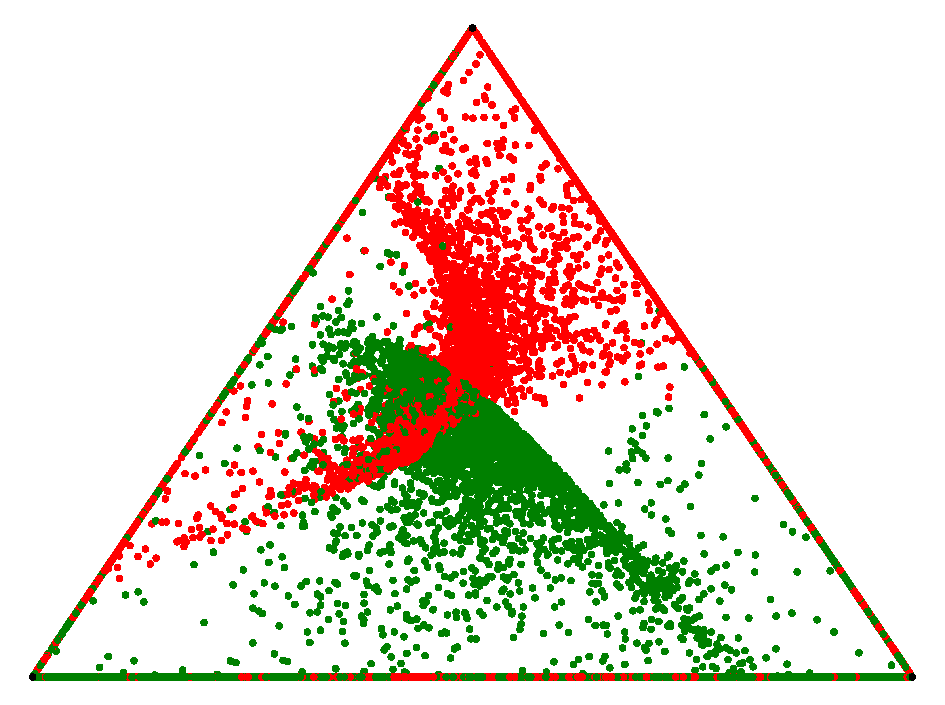
\includegraphics[width=\textwidth]{Pictures/paretoNash-curvyRegionsManyOutliers-k5}
            \caption{Zero-Sum Game, $m=5$}
        \end{subfigure}
        \begin{subfigure}[t]{0.49\textwidth}
            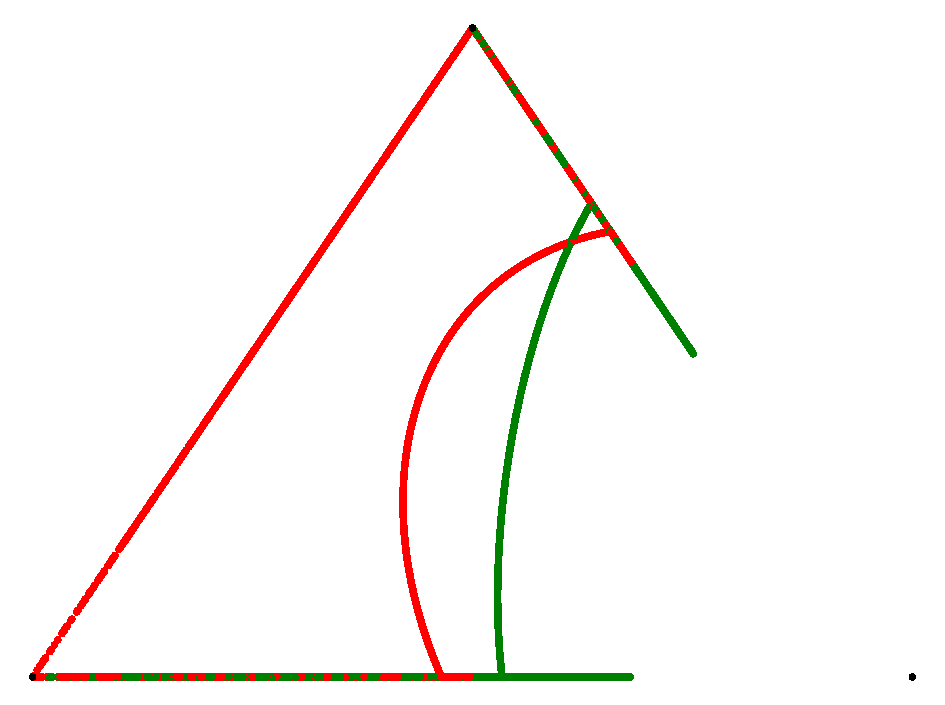
\includegraphics[width=\textwidth]{Pictures/paretoNash-curves1-k2}
            \caption{Zero-Sum Game, $m=2$}
        \end{subfigure}
        
        \vspace*{0.01\textwidth}
        
        \begin{subfigure}[t]{0.49\textwidth}
            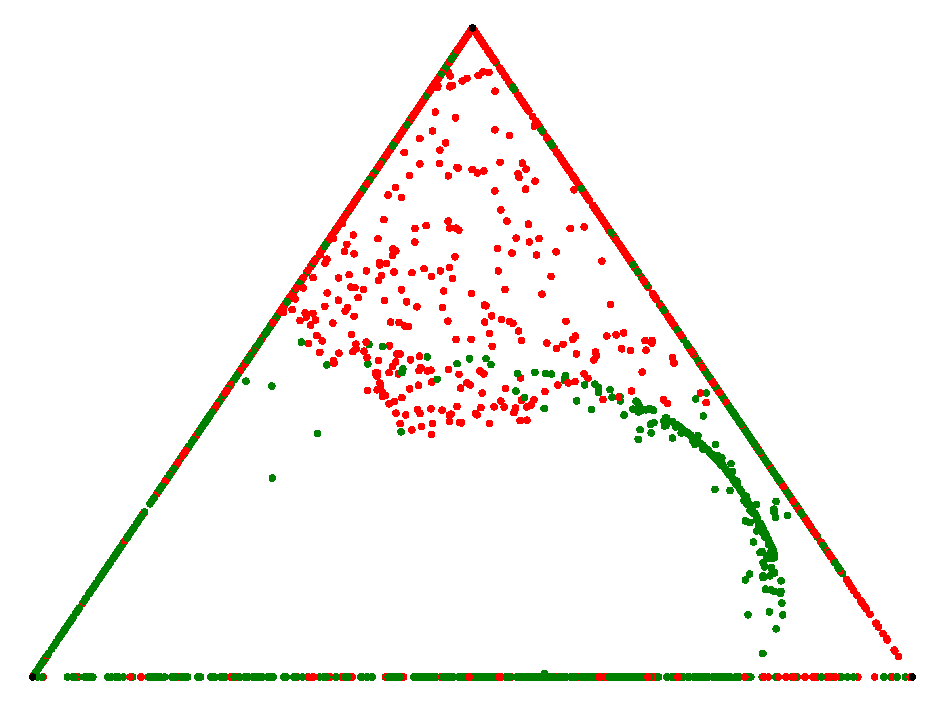
\includegraphics[width=\textwidth]{Pictures/paretoNash-bimatrix-k3}
            \caption{Non-Zero-Sum Game, $m=3$}
        \end{subfigure}
        \begin{subfigure}[t]{0.49\textwidth}
            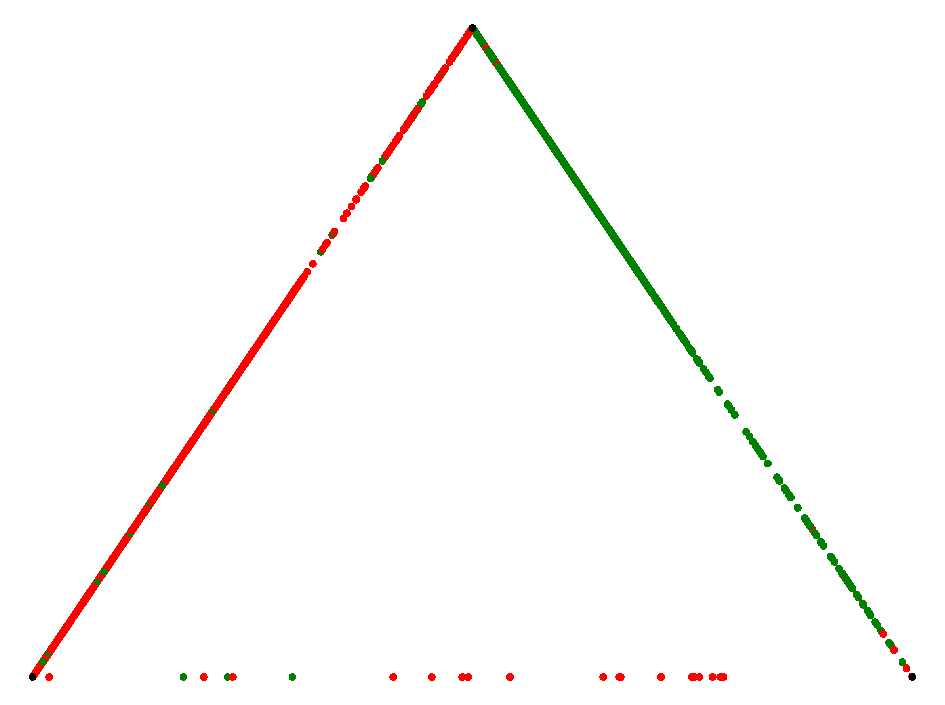
\includegraphics[width=\textwidth]{Pictures/paretoNash-emptyCenter-k5}
            \caption{Zero-Sum Game, $m=5$, no equilibria mixing between all three strategies found}
        \end{subfigure}
%        \vspace*{0.01\textwidth}
%        
%        \begin{subfigure}[b]{0.49\textwidth}
%            \includegraphics[width=\textwidth]{Pictures/paretoNash-clusters-k5.pdf}
%            \caption{}
%        \end{subfigure}
%        \begin{subfigure}[b]{0.49\textwidth}
%            \includegraphics[width=\textwidth]{Pictures/paretoNash-denseCurvyRegions-k3.pdf}
%            \caption{}
%        \end{subfigure}
%        
%        \vspace*{0.01\textwidth}
%        
%        \begin{subfigure}[b]{0.49\textwidth}
%            \includegraphics[width=\textwidth]{Pictures/paretoNash-curves2-k2.pdf}
%            \caption{}
%        \end{subfigure}
%        \begin{subfigure}[b]{0.49\textwidth}
%            \includegraphics[width=\textwidth]{Pictures/paretoNash-scatteredWithLines-k5.pdf}
%            \caption{}
%        \end{subfigure}
        \caption{Different sets of Pareto-Nash equilibria visualized (10\,000 points each)}
        \label{fig:paretoNashEquilibriaShowcase}
    \end{figure}

    \subsection{Multi-Objective Segmented-Distribution Games}
    Putting the pieces together, we construct the multi-objective game based on loss distribution segments as follows:
    % TODO watch out, here we use indices 1...m, above we used 1...n
    Let $G$ be a mixed-extension distribution-valued game with outcomes from $\Fab$, $a < b$, and let $\mathcal{I} = \set{a, x_2, x_3, \dots, x_m, b}$ be a partition of the interval $[a, b]$.
    
    \newcommand{\Gseg}[1][]{G_{\text{seg,$\ifstrempty{#1}{\mathcal{I}}{#1}$}}}
    Define the \emph{segment game} $\Gseg$ as a multi-objective game with the same strategies as in $G$, where each player $k$ has the utility function:
    \begin{gather}
        u_{\text{seg}, k}: S \to \R^m, s \mapsto -\bigpars{E_{[x_1, x_2)}(u_k(s)), E_{[x_2, x_3)}(u_k(s)), \dots, E_{[x_m, b]}(u_k(s))}
        \label{eq:segmentsExpectationVector}
    \end{gather}
    We are negating the vector as we are in the context of loss distributions, but want to stick to the convention that utilities should be maximized.
    As outlined in the previous section, we can find Pareto-Nash equilibria  of $\Gseg$ by weighting the different objectives and then solving the resulting real-valued game.
    This approach is implemented for the thesis in the language \texttt{R}, and the following describes the details of the implementation.
    
    % TODO cite something about HyRiM?
    The \texttt{R} package \emph{HyRiM}  by Stefan Rass, Sandra König and Ali Alshawish was developed along with the papers \cite{bib:rassGameRiskManagI,bib:rassGameRiskManagII,bib:rassGameRiskManagIII} and implements algorithms and data structures for distribution-valued games.
    In particular, it can represent loss distributions either of finitely-supported discrete or of absolutely continuous nature, where absolutely continuous distributions are approximated by a kernel density estimation method. Besides loss distributions, it also has a class that represents distribution-valued games, and implements the computation of Nash equilibria for real-valued games.
    
    We implement the multi-objective segmentation-based games in the context of the HyRiM package, and as a possible extension to it. As the package focuses on zero-sum games, we also restrict ourselves to zero-sum segmented games.
    Multi-objective segmented games are represented by the \texttt{moseg} class. Such a game can be created from a single-objective distribution-valued game, represented in HyRiM by the \texttt{mosg} class, and a vector of partition points.
    Loss distributions are turned into real-valued expectation vectors by \eqref{eq:segmentsExpectationVector}: this is implemented in the function \texttt{segmentedLossDistribution}, which takes in a \texttt{lossDistribution} object and the partition points and returns the expectation vector.
    Computing the expected value is straightforward in the case of finitely-supported discrete distributions as a sum; for absolutely continuous distributions, numerical integration is used 
    (however this is not implemented yet).
    Finally, the method \texttt{moseg.paretoNashEquilibrium} computes a Pareto-Nash equilibrium of a game of the \texttt{moseg} class, given a vector of weights as inputs.
    It first scalarizes the game based on the weights.
    Then for the actual equilibrium computation, it utilizes the HyRiM built-in method \texttt{mgss} which besides distribution-valued games supports equilibrium computation for real-valued games.
    
    \paragraph{Creation of Segmented Game}
    The code for creating a \texttt{moseg} game:
    
    \lstset{showspaces=false,
        keywordstyle=\ttfamily\bfseries\color{purple},
        basicstyle=\ttfamily,
        numbers=left,
        numberstyle=\tiny,
        commentstyle=\color{gray},
        breaklines=true,
        postbreak=\mbox{\textcolor{lightgray}{$\hookrightarrow$}\space},
        showstringspaces=false,
        stringstyle=\color{brickred},
    }
    \lstinputlisting[language=R, firstline=13, lastline=31]{../Experiments/leqtw-multiobjective/multiobjectiveSegmentGame.R}
    
    \paragraph{Computing Expectation Vectors}
    The code for converting a \texttt{lossDistribution} in a segment expectation vector:
    \lstinputlisting[language=R, firstline=67, lastline=96]{../Experiments/leqtw-multiobjective/multiobjectiveSegmentGame.R}
    
    \paragraph{Computing Pareto-Nash Equilibria}
    The code for computing Pareto-Nash equilibrium of a \texttt{moseg} based on weights:
    \lstinputlisting[language=R, firstline=42, lastline=55]{../Experiments/leqtw-multiobjective/multiobjectiveSegmentGame.R}
    
    
%    \chapter{Distribution-Valued Game Theory in Security of Critical Infrastructures}
    
%    \nocite{*}
    \printbibliography
\end{document}